%
% IEEE Transactions on Microwave Theory and Techniques example
% Tibault Reveyrand - http://www.microwave.fr
%
% http://www.microwave.fr/LaTeX.html
% ---------------------------------------
\documentclass[journal]{IEEEtran}
%\usepackage[retainorgcmds]{IEEEtrantools}
%\usepackage{bibentry}  
\usepackage{xcolor,soul,framed} %,caption

\colorlet{shadecolor}{yellow}
% \usepackage{color,soul}
\usepackage[pdftex]{graphicx}
\graphicspath{{../pdf/}{../jpeg/}}
\DeclareGraphicsExtensions{.pdf,.jpeg,.png}

%Mathabx do not work on ScribTex => Removed
%\usepackage{mathabx}
\usepackage{array}
\usepackage{mdwmath}
\usepackage{mdwtab}
\usepackage{eqparbox}
\usepackage{url}
\usepackage{amsmath}
\usepackage{amssymb}
\usepackage{cite}
\usepackage{pdfpages}
\usepackage{booktabs}
\usepackage{placeins}
% \usepackage{graphicx}
\usepackage{multirow}
\DeclareMathOperator*{\argmin}{argmin}
\usepackage[colorlinks=true, allcolors=blue]{hyperref}


\hyphenation{op-tical net-works semi-conduc-tor}

%\bstctlcite{IEEE:BSTcontrol}


%=== TITLE & AUTHORS ====================================================================
\begin{document}
\bstctlcite{IEEEexample:BSTcontrol}
    \title{A Weakly-Supervised Semantic Segmentation Approach Based on a Closed-Form Matting Solution}
   	\author{Kai Yao, Alberto Ortiz, and Francisco Bonnin-Pascual,
\thanks{Department of Mathematics and Computer Science (University of the Balearic Islands) and IDISBA (Institut d'Investigacio Sanitaria de les Illes Balears), Palma de Mallorca, Spain; \{k.yao, alberto.ortiz, xisco.bonnin\}@uib.es}}
% ====================================================================
\maketitle


% === ABSTRACT ====================================================================
% =================================================================================
\begin{abstract}
%\boldmath
Weakly-supervised semantic segmentation is a challenging task owing to the complex content with non-uniform intensity distribution, diversity of targets, and lacking the sufficient and accurate ground truth. In order to overcome these challenges, we propose and assess a novel scribble-based weakly-supervised semantic segmentation solution by employing a closed-form matting loss function, namely closed-form matting (CFM) loss, which aims at propagating the semantic information from user annotations to unknown areas. Our solution only needs scribble annotations to train a segmentation network. Addressing the Multi-Category problem, a simple network, namely Multi-Label Classification (MLC) model, is proposed and integrated into the segmentation backbone. The performance of our approach is evaluated against datasets from two different industry-related inspection tasks: one task is designed to detect the marine creature attached to the hull of vessels through photos taken underwater; another task is to deal with the localization of image areas whose pixels correspond to scene surface points affected by a specific sort of defect. Besides, two datasets from PASCAL VOC and CityScape benchmarks are used to evaluate the performance of our solution for the multi-category problem. Experimental results exhibit that our approach can obtain reasonable segmentation performance only using scribble annotations.
\end{abstract}

% === KEYWORDS ====================================================================
% =================================================================================
\begin{IEEEkeywords}
% \hl{Object recognition, inspection, closed-form image matting, and weakly-supervised semantic segmentation}
Object recognition, inspection, closed-form image matting, and weakly-supervised semantic segmentation
\end{IEEEkeywords}
% For peer review papers, you can put extra information on the cover
% page as needed:
% \ifCLASSOPTIONpeerreview
% \begin{center} \bfseries EDICS Category: 3-BBND \end{center}
% \fi
%
% For peerreview papers, this IEEEtran command inserts a page break and
% creates the second title. It will be ignored for other modes.
\IEEEpeerreviewmaketitle


% === I. INTRODUCTION =============================================================
% =================================================================================
\section{Introduction}
\label{intro}
Image semantic segmentation is a fundamental problem in the computer vision area, which refers to a pixel-level classification problem. The most prevalent approach to training semantic segmentation models is full supervision, where the pixel-label annotations are used to train. Via the fully supervised semantic segmentation (FSSS) approach, complicated targets, boundary detection, and localization information can be obtained based on pixel-level segmentation results. 

Recently, the success of vision tasks based on the end-to-end training of deep convolutional neural network (DCNN) gives researchers the enthusiasm to explore DCNN-based segmentation. Comparing to the approaches using hand-crafted features, DCNN-based approaches have the capacity to automatically learn the representation through a set of multi-scale feature maps defined in the architecture and a number of convolutional filters. 

Although the FSSS approaches have accomplished state-of-the-art performance \cite{chen2017deeplab,hariharan2015hypercolumns,chen2017rethinking,long2015fully} on several benchmarks, one difficulty that prevents the FSSS approaches from being widely used is that it needs numerous pixel-wise annotations, which is expensive and time-consuming in reality. Therefore, pixel-wise annotations are regarded as the key to the success of the segmentation tasks. Addressing this problem, the weakly-supervised semantic segmentation (WSSS), only using partial annotations or image-tags to train the segmentation network, is regarded as the solution. In this work, a scribble-based WSSS solution is proposed from which training masks are derived from propagating the semantic information from labelled pixels to unlabelled pixels. 
% Automated surface inspection (ASI) using computer vision techniques is a critical task in industry, which is widely used to automatically inspect defects on the vessel surface, such as corrosion, holes, scratches, and pits. The extant ASI algorithms focus on detecting four kinds of surfaces: (1) non-textured surface; (2) repeated pattern surface; (3) homogeneously textured surface; and (4) non-homogeneously textured surface \cite{xie2008review}. However, these approaches highly depend on the man-crafted features. Therefore, the shortcomings of these methods are obvious: (1) sensitive to changes of the background, (2) dependent on human knowledge, and (3) constrained to the robustness and generalization of man-crafted features. 

% Recently, the success of vision tasks based on the end-to-end training of deep convolutional neural network (DCNN) gives researchers the enthusiasm to explore the DCNN-based application. Comparing to the traditional ASI solutions, the DCNN-based approach has a critical advantage where it can automatically learn high-level features from the training data and classify defects at the same time without the need for hand-crafted features. Furthermore, the DCNN-based approach is robust to variations and versatile, allowing inspection of different types of surfaces and defects. Especially for semantic segmentation, the DCNN-based approaches \cite{chen2018encoder,long2015fully} are more effective in improving the detection performance than previously proposed methods. 
% weak seg
% Therefore, the WSSS problem has become to reconstruct the fully labelled mask from partially labelled mask, namely, recovering mask containing missing regions. 
The challenge of the WSSS problem is to use sparse ground truth to obtain compact and accurate segmentation results. Only using weak annotations to train the segmentation network, the results tend to be very sparse, even predict all pixels belong to the background \cite{zhang2019survey}. Nowadays, the popular methods for the WSSS problem are based on Classification Activation Maps (CAMs) \cite{zhou2016learning}. Given training images with only image-level class labels, a classification model is trained, and the class-specific seed areas are obtained during inference. Then, the CAMs are expanded to obtain the Pseudo-Masks \cite{huang2018weakly,wei2018revisiting,wang2020self}, which are used to train a fully supervised semantic segmentation model. However, the CAMs often confuse part of the detected target with background, which is inherited in the segmentation stage.

Scribbles are another kind of economic segmentation ground truth, which is considered as a user-friendly and efficient annotation. Scribble annotations only need the user to drag the cursor in the area of targets, and it need not the whole outline of targets. Thus, scribble annotations avoid inaccurate segmentation cues compared to the CAMs-based approach. 

Therefore, this work focuses on using scribble annotations to obtain accurate pixel-wise segmentation for two main tasks. The first one refers to the two industry-related inspection tasks, and the second one is for two multi-category semantic segmentation (MCSS) tasks. Regarding the two inspection tasks, one task is to detect corrosion on the tank surface of vessels (COR task), and another is to detect BioFouling on the vessel's hull (BIO task). In the marine environment, steel materials are prone to severe corrosion and biological contamination, and their damage not only affects the normal operation of vessels but also seriously decreases the lifespan of vessels. Our solution aims at providing an automatic vision-based inspection approach. On the other hand, the inspection tasks only need to detect one category target (corrosion and BioFouling). In order to verify our approach, two multi-category datasets are extracted from Pascal VOC 2012 \cite{everingham2012pascal} and CityScapes \cite{cordts2016cityscapes}. 

% CFM approach
For the scribble-based WSSS problem, a closed-form matting (CFM) solution is proposed in this work. Closed-form matting \cite{levin2007closed} applies the alpha-color model, which establishes the relationship between the color value and alpha value of each pixel, and it propagates the user annotations to the entire image via minimizing a quadratic cost function. Then, a sparse linear system, where the matting Laplacian matrix is constructed using input image and scribble annotations, is built and solved to obtain the closed-form alpha matte. Considering our problem, the normalized alpha-value from the CFM approach can be seen as the pixel-wise segmentation for one category. Furthermore, a DCNN-based segmentation network trained by the quadratic loss is used to get the optimal alpha solution. 

The main contribution of this work are summarized as follows:
\begin{itemize}
    \item A new loss function (namely closed-form matting loss) aiming at solving the scribble-based WSSS problem is applied to overcome challenges due to ambiguous and sparse annotations.
    \item A multi-label classification (MLC) model is developed to implement the CFM loss to the MCSS task.  
    % \item A segmentation model-based solution using the Closed-Form Loss is proposed to solve our two inspection tasks. 
    \item Some segmentation networks trained with the closed-form matting loss have experimented in this work, and they obtained considerable performance.
    \item We assess the performance of the matting and segmentation performance on a benchmark comprising two industry-related inspection applications and two MCSS tasks.
\end{itemize}

This paper is organized as follows: Section \ref{related} briefly reviews some previous works for the WSSS problem; Section \ref{method} introduces the methodology of our solution in detail; Section \ref{exp_dis} reports on the results of a number of experiments aiming at showing the performance of our approach, and Section \ref{conclusion} concludes this work. 

\section{Related Work}
\label{related}
Numerous FSSS approaches have already been proposed and have achieved impressive performance. Unlike the FSSS problem, which requires plenty of pixel-level ground truth and turns out to be very costly in practice, the WSSS aims at using the partial or image-tag label to get the reasonable, even same segmentation performance as FSSS approaches. Actually, the performance of FSSS approaches is far higher than that of WSSS approaches. Nonetheless, the quality of WSSS methods is impressive, especially considering that learning to segment with a few or without any location-specific supervision is a challenge but brings massive efficiency in the industry scenario. We broadly classified the WSSS problem into three categories according to the class of weak annotations, which are image-tag labels, bounding boxes-based annotations, and scribble-based annotations. 

% However, due to lacking the accurate and intensive target-related seeds from CAMs, their approach does not perform well for small and sparse targets.
Since image-tag labels completely lack the localization information, most current approaches have two-stage, i.e., generate accurate pseudo ground truth firstly, then use the pseudo labels to train a segmentation network. Typically, SEC \cite{kolesnikov2016seed} proposed three loss functions, called seeding, expansion, and boundary constrain losses, to expand the initial seeds obtained from CAMs \cite{zhou2016learning} and train the FCN-based model. DSRG \cite{huang2018weakly} develops a DCNN-based seed region growing strategy to progressively extend the detected region during training. Their approach starts from the discriminative regions from CAMs, then the region growing module is integrated into a deep segmentation network to obtain a complete segmentation. Then, IRNet \cite{ahn2019weakly} is designed for both semantic and instance segmentation. Similarly, their approach uses CAMs as pseudo ground truth, and two branches extending from the backbone are used to predict auxiliary information and the segmentation results. 

Some researchers consider that the key factor of the WSSS problem of image-tag labels is to obtain high-quality CAMs. AffinityNet \cite{ma2019affinitynet} is proposed to learn semantic affinities among adjacent pixels using a limited number of training samples. Additionally, a k-Nearest-Neighbor (kNN) attention pooling layer is applied to decide its k-nearest neighbors, which ensures similar nodes have similar node representation. Stacking kNN attention pooling layers, the AffinityNet can transfer the semantic information from known pixels to their adjacent unknown pixels. In \cite{choe2019attention}, an Attention-based Dropout Layer (ADL) is developed to obtain the entire outline of the target from CAMs. The ADL relies on a self-attention mechanism to process the feature maps. Particularly, during training, this layer hides the most discriminating parts in the feature maps, which induces the network to learn the less discriminating parts while it highlights the informative region of the target to improve the recognition ability. Alternatively, Wei et al. \cite{wei2018revisiting} find that varying dilation rates can effectively transfer the discriminative information to non-discriminative regions, promoting the emergence of these regions in CAMs. 

Regarding the use of bounding boxes as weakly-supervised annotations for semantic segmentation, in \cite{khoreva2017simple}, the authors combine two traditional segmentation approaches (GraphCut and Holistically-nested Edge Detection (HED)) algorithms with DCNN to refine the bounding boxes ground truth and make predictions, then the refined ground truth is used to train the network iteratively. An FCN-based network is proposed in \cite{song2019box} to obtain the segmentation results using bounding boxes annotation. Particularly, the authors consider the filling rate, which is the ratio between the size of the target and the size of bounding box annotation, as helpful guidance for obtaining reasonable segmentation performance. Firstly, an FCN and a dense CRF \cite{krahenbuhl2011efficient} are used to get the segment proposals, then they propose a box-driven class-wise region masking (BCM) and filling rate guided loss (FR-loss) to train the network. Differently, Hsu et al. \cite{hsu2019weakly} view the bounding boxes-based WSSS problem as a multiple instance learning (MIL) task. They generate positive and negative bags based on the sweeping lines from the bounding box annotations. The MIL formulation obtains the instance segmentation results by leveraging the tightness property of bounding boxes. Therefore, latent pixel-wise labels, the object instance feature representation, and the segmentation model can be derived simultaneously. 

On the other hand, scribbles are another widely used weak annotation for semantic segmentation, which is recognized as one of the most user-friendly ways for labelling. This topic has been explored through graph cuts \cite{boykov2001interactive}, random walks \cite{grady2006random}, and weighted geodesic distances \cite{bai2009geodesic}. As an improvement, \cite{tang2018regularized} develops two regularization terms based on Normalized Cuts and dense CRF. In another work \cite{wang2019boundary}, a Boundary Perception Guidance (BPG) is proposed, which consists of two components, i.e., prediction and boundary regression. Accordingly, the network has a Prediction Refinement Network (PRN) sub-network to predict the segmentation results using scribble annotations, and the Boundary Regression Network is used to guide the network to extract edge features using class-agnostic maps as supervision. Besides, Yao et al. \cite{yao2021weakly} apply two kinds of weak annotations (scribbles and pseudo-masks) to train the Attention U-Net \cite{oktay2018attention} for image semantic segmentation. The hierarchical WSSS model consists of two tasks: a. the authors augment the scribble ground truth and train the network to get segmentation results; b. the k-means clustering with scribble annotations is trained in the sub-network, which is used to assist the segmentation task. 
% get the initial substructure segmentation, which is used to train another U-Net to segment targets.

Our work falls into the scribble-based WSSS problem. In particular, a deep semantic segmentation network is used to optimize a quadratic loss function to obtain the closed-form solution of a sparse linear system. A specific loss function is designed to propagate the semantic information from the labelled pixels to the unknown label region. Experiments show that our approach is effective in segmenting targets under scribble annotation. 


\section{Methodology}
\label{method}
The methodology of our solution is introduced in this section. Firstly, a brief illustration of the closed-form solution for image matting \cite{levin2007closed} is presented in Section \ref{subsec:background}. Then, the CFM loss is demonstrated in Section \ref{subsec:closed-form-loss}. The scribble-based weak annotations used in our solution are introduced in Section \ref{subsec:weak-annotations}. Addressing the MCSS problem, the MLC model is introduced in Section \ref{subsec:mlc_model}. Finally, we introduce some segmentation networks as the backbone of our approach in \ref{subsec:seg_backbone}, including DeepLabV3+ \cite{chen2018encoder}, U-Net \cite{ronneberger2015u}, and ERFNet \cite{romera2017erfnet}.
\subsection{Background}
\label{subsec:background}
For a gray image, the gray-scale value ($I_i$) of each pixel can be represented as,
\begin{equation}
    I_i = \alpha_{i} F_{i} + (1 - \alpha_{i})B_{i}
    \label{func_Ii}
\end{equation}
where $F$ represents the foreground, $B$ represents the background, and $\alpha$ denotes the alpha channel. Redoing (Eq. \ref{func_Ii}), we can get the expression as follow.
\begin{equation}
    \alpha_{i} = \frac{1}{F_{i} - B_{i}}I_{i} + (-\frac{B_{i}}{F_{i} - B_{i}}) 
    \label{func_alphai}
\end{equation}
Some assumptions on the nature of $F_i$, $B_i$ and $\alpha_i$ are needed. Assume that both $F_i$ and $B_i$ are approximately constant over a small window around  each pixel. This assumption allows us to rewrite (Eq. \ref{func_alphai}), expressing $\alpha$ as a linear function of image $I$ in Eq. \ref{func_alphai_2},
\begin{equation}
    \alpha_{i} \approx a_{i} I_{i} + b_{i}, \forall i\in w
    \label{func_alphai_2}
\end{equation}
where $a_i = \frac{1}{F_{i}-B_{i}}$, $b_i = -\frac{B_{i}}{F_{i}-B_{i}}$, and $w$ is a small image window, whose size is $3\times 3$ as usual. So the relation suggests finding $\alpha$, $a_i$ and $b_i$ that minimizes the cost function as below,
\begin{equation}
    J(\alpha, a_i, b_i) = \sum\limits_{j\in k}\left(\sum\limits_{i\in w_{k}}(\alpha_{i} - a_{j}I_{i} - b_{j})^{2} + \epsilon a_{j}^{2}\right)
    \label{func_j_alpha_a_b}
\end{equation}
where $w_k$ is a small window around pixel $j$. The cost function in Eq. \ref{func_j_alpha_a_b} includes a regularization term on $a$. One reason for this term is numerical stability \cite{levin2007closed}.

The cost function is quadratic in $\alpha$, $a_i$, and $b_i$, with $3N$ unknowns for an image with $N$ pixels. Through several derivations, $a_i$ and $b_i$ can be removed from Eq. \ref{func_j_alpha_a_b}, leaving us with a quadratic cost in only $N$ unknowns: the $\alpha$ values of the pixels,
\begin{equation}
    J(\alpha) = \alpha^T L \alpha
    \label{func_quadratic_cost}
\end{equation}
where, $L$ is the Matting Laplacian matrix, whose size is $N\times N$. The $(i,j)$th entry is,
\begin{equation}
    \hspace*{-0.5cm}
    \sum\limits_{k|(i,j)\in w_k} \left( \delta_{ij} - \frac{1}{|w_k|} \left( 1 + \frac{1}{\frac{\epsilon}{|w_k| + \sigma_k^2}} (I_i - \mu_k) (I_j - \mu_k) \right) \right)
    \label{laplacian_entry}
\end{equation}
where, $w_k$ presents a small window of $3\times 3$ pixels. Since we place a window around each pixel, the window, $\mu_k$ and $\sigma_k^2$ are the mean and variance of the intensities in the window $w_k$ around $k$, and $|w_k|$ is the number of pixels in this window. $\delta_{ij}$ is the Kronecker delta as shown below.
\begin{equation}
    \delta_{ij} = \left \{
        \begin{aligned}
            &0,~~~\text{if}~i \neq j \\
            &1,~~~\text{if}~i = j \\
        \end{aligned}
    \right .
    \label{Kronecker delta}
\end{equation}

The alpha value for color image, a BGR image for instance, also can be obtained by optimizing the quadratic form loss as Eq. \ref{func_quadratic_cost}. The $(i,j)$th entry of the Matting Laplacian Matrix is,
\begin{equation}
    \hspace*{-0.2cm}
    \sum\limits_{k|(i,j)\in w_k} \left( \delta_{ij} - \frac{1}{m} \left( 1 + (I_i - \mu_k)^T \left( \Sigma_k + \frac{\epsilon I_{3}}{m} \right) (I_j - \mu_k)  \right) \right)
    \label{laplacian_entry_bgr}
\end{equation}
where, $I_3$ is a $3\times 3$ identity matrix, $\mu_k$ is the $3\times 1$ mean value of colors in window $w_k$, $\Sigma_k$ is the $3\times 3$ covariance matrix of the intensities in window $w_k$. 

To provide the user with more flexible control over the output, the scribble annotations are used for the constraint priors. In order to extract an alpha matte matching the user's constraints, the optimized problem has become to find the optimal $\alpha^{*}$ in Eq. \ref{optimize_alpha}.
\begin{equation}
    \alpha^{*} = \argmin\limits_{\alpha} \left[ \alpha^T L \alpha + \lambda (\alpha - S)^T D_s (\alpha - S) \right]
    \label{optimize_alpha}
\end{equation}
where, $D_s$ is a diagonal matrix whose diagonal elements are one for constrained pixels and zero for all other pixels, $S$ is the vector containing the specified alpha values for the constrained prior and zero for all other pixels, and $\lambda$ is a large number (100 in our experiments). 

As can be seen, the loss function in Eq. \ref{optimize_alpha} is a quadratic in $\alpha$, the optimal solution can be found by \textit{Lagrange multiplier}. In the end, this is equivalent to solving the following sparse linear system in Eq. \ref{sparse_linear_system}.
\begin{equation}
    (L + \lambda D_s) \alpha = \lambda S
    \label{sparse_linear_system}
\end{equation}

\subsection{Closed Form Matting Loss Function}
\label{subsec:closed-form-loss}
As known in Eq. \ref{optimize_alpha}, the optimal solution $\alpha*$ can be obtained by solving the sparse linear system in Eq. \ref{sparse_linear_system}. Inspired by the success of DCNN-based models, we consider using a DCNN to predict the $\alpha$ in Eq. \ref{sparse_linear_system}, and change the original optimized problem to a DCNN-based learning problem. Note that the matting problem in \cite{levin2007closed} needs two inputs (image and scribble annotations) to obtain the optimal solution. After changing to a learning problem, the DCNN-based model only needs one input image to obtain the final solution with less running time during inference. Therefore, our DCNN-based solution is more efficient and requires fewer inputs.

Specifically, we use a Mean Square Error (MSE) loss function with a DCNN-based model to obtain the approximate optimal solution. The loss function are modified based on Eq. \ref{sparse_linear_system}, and it can be expressed in Eq. \ref{mseloss_closed_form}.
\begin{equation}
    L_{\text{cfm}}(\alpha, \theta) = ||(L+\lambda D_s) \alpha(\theta) - \lambda D_s S||^2
    \label{mseloss_closed_form}
\end{equation}
where, $\theta$ represents the weights of the segmentation model, and $\alpha$ denotes the network prediction. The definitions of $L$, $D_s$, and $S$ are the same as in Eq. \ref{optimize_alpha}, which can be obtained from the input image and constraint priors (scribble annotations).

Let $A = L+\lambda D_s$ and $B = \lambda D_s S$, so the loss function in Eq. \ref{mseloss_closed_form} can be simplified as follow. 
\begin{equation}
    L_{\text{cfm}}(\alpha, \theta) = ||A \alpha(\theta) - B||^2
    \label{closed_form_loss_one_channel}
\end{equation}

In Eq. \ref{closed_form_loss_one_channel}, $\alpha$ is the prediction of one category and $w_c$ denotes the weight for every category, which is used to solve the imbalance problem between different categories. For the multi-category problem (assuming $C$ categories), the loss function can be expressed as:
\begin{equation}
    L_{\text{cfm}}(\alpha_c, \theta, w_c) = \frac{\sum\limits_{c=1}^{C} ||w_c(A_c \alpha_{c}(\theta) - B_c)||^2}{C},~~c\in C
    \label{closed_form_loss_mul_channel}
\end{equation}
where $A_c = L + \lambda D_{s,c}$, $B_c = \lambda D_{s,c}$.

\subsection{Scribble Annotations}
\label{subsec:weak-annotations}
In our system, we apply the scribbles-based weak annotations as the prior constraints. Let $\alpha_{gt}$ be the scribble annotations for category $c$, which can be formally defined in Eq. \ref{scribble_define_eq}, 
\begin{equation}
    \alpha_{gt,c}(x, y) =
    \begin{cases}
      0, \text{background} \\
      128, \text{unknown} \\
      255, \text{foreground} \\ 
    \end{cases}, ~~~~c\in~C
    \label{scribble_define_eq}
\end{equation}
where $(x, y)$ indicates the coordinates of pixel in the image. Intuitively, the scribble annotations separate the semitransparent regions from the opaque foreground and background. In order to obtain the optimal $\alpha^*$, the matting approach naturally divided two steps: a. decide pixels to belong foreground or background for labelled pixels; b. compute the alpha value for a pixel locates in the unknown regions. Reminiscent the WSSS task, whose target is to divide the image into discrete parts according to the semantic information, the partial matting alpha (scribble) annotation is helpful for the segmentation task in two aspects. On the one hand, propagating the $\alpha$ value for unlabelled pixels can significantly relieve the burden of the network to predict the extracted label for these pixels. On the other hand, the labelled pixels can provide prior knowledge for the network and also enhance the regression performance of the network for these labelled pixels. Besides, if the user annotations contain minor errors, the propagation mechanism would like to correct them. 

Figure \ref{fg:weak-annotations} shows four example pictures of our tasks. As can be seen, the unknown region in the scribble annotations is vast and erroneous, while only a few  pixels are labelled. Rightfully, directly using scribble annotations to train segmentation network cannot achieve satisfactory performance, even does not converge. However, our approach can obtain precise matte and segmentation results, thus perfectly solves our problems. 
\begin{figure}[t]
    \centering
    \begin{tabular}{@{\hspace{0mm}}c@{\hspace{1mm}}c@{\hspace{1mm}}c@{\hspace{0mm}}}
        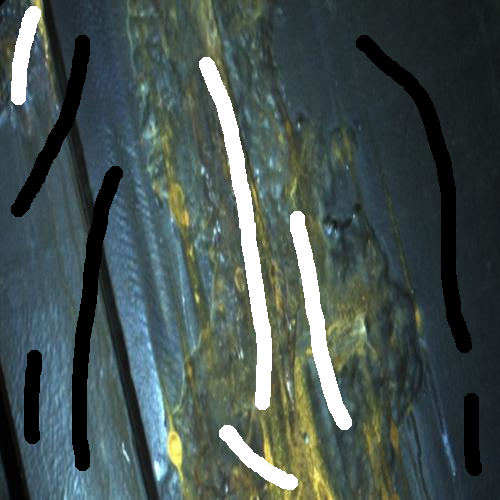
\includegraphics[width=0.3\columnwidth, height=0.3\columnwidth]{imgs/gk2_fp_exp28_0380_30_ROI.png} &
        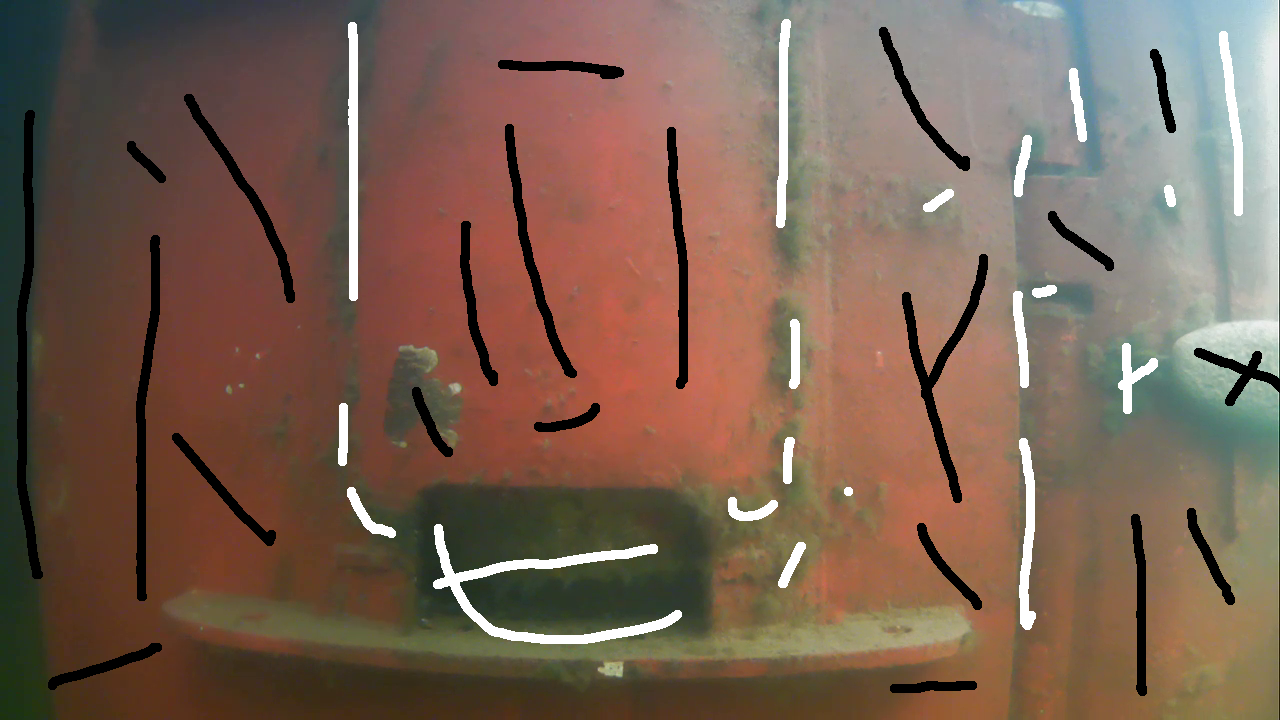
\includegraphics[width=0.3\columnwidth, height=0.3\columnwidth]{imgs/beye_01_001900.png} \\
        \footnotesize (a) & \footnotesize (b) \\
        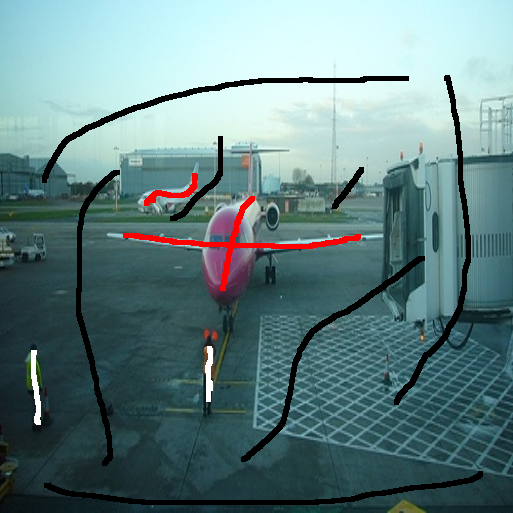
\includegraphics[width=0.3\columnwidth, height=0.3\columnwidth]{imgs/2007_000032.png} &
        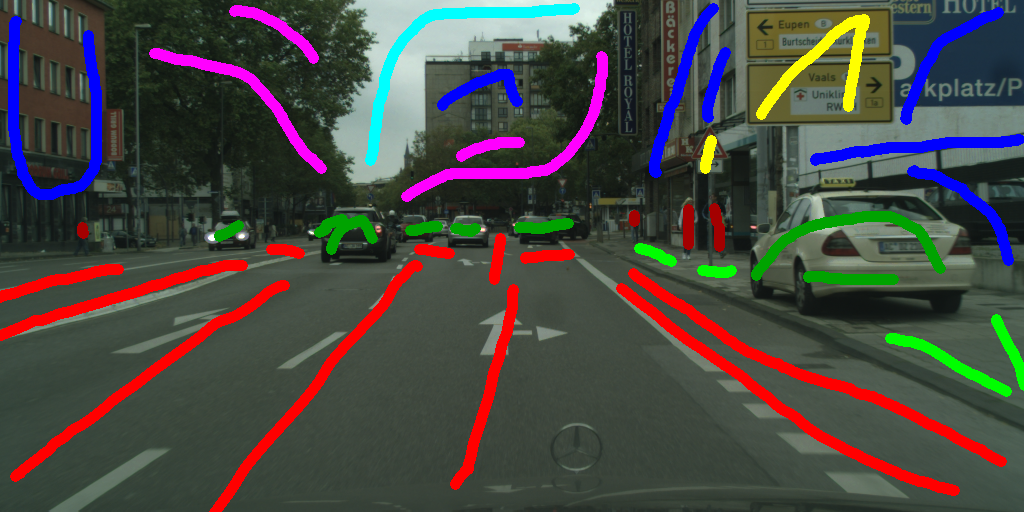
\includegraphics[width=0.3\columnwidth, height=0.3\columnwidth]{imgs/aachen_000005_000019_leftImg8bit.png}\\
        \footnotesize (c) & \footnotesize (d) \\
    \end{tabular}
    \caption{Samples of weak annotations, from more to less informative: (a) and (b) are samples from the inspection tasks, and only black and white scribbles are used due to the binary segmentation task; (c) and (d) come form the MCSS tasks, and different color scribbles are used to distinguish the category of target.}
    \label{fg:weak-annotations}
\end{figure}

\subsection{Multi-Label Classification}
\label{subsec:mlc_model}
In order to solve the Multi-Label problem, a simple Multi-Label Classification (MLC) model is developed, which consists of an average pooling layer, two Fully-Connected (FC) layers, and a Sigmoid activation function. The MLC model is connected with the encoder, as shown in Fig. \ref{mseloss_closed_form}. During training, we employ a Cross-Entropy Loss to train the MLC model. Regarding the classification ground truth, the scribble annotation can provide the information of the targets' category appeared in the image. 

In the end, the loss function ($L$) of multi-label problem is shown as follow,
\begin{equation}
    \begin{aligned}
        L &= L_{\text{cfm}} + \beta L_{\text{MLC}}, \\
        L_{\text{MLC}} &= \sum\limits_{c}^{C} y_c \log(p_c) + (1 - y_c) \log(1 - p_c)
    \end{aligned}
    \label{loss_multi_class}
\end{equation}
where $C$ represents the number of categories, $\beta$ is the trade-off constant,  $y_c$ indicates the ground truth and $p_c$ denotes the output of MLC model.

\subsection{Segmentation Backbones}
\label{subsec:seg_backbone}
For the task of semantic segmentation, the spatial pyramid pooling module and auto encoder-decoder structure are widely used in deep neural networks. The spatial pyramid pooling module can encode multi-scale contextual information by probing the incoming features with filters or pooling operations at multiple rates and multiple effective fields-of-view. While the auto decoder model makes full use of the multi-scale and rich semantic information features from DCNN, which is helpful to obtain an accurate target profile. In this section, we introduce different segmentation networks as the backbones in our solution in order to validate the effectiveness of our approach.

\subsubsection{DeepLabV3+}
DeepLabV3+ \cite{chen2018encoder} extends the DeepLabV3 \cite{chen2017rethinking} by adding a practical decoder module to refine the segmentation results. The DeepLabV3+, applied in this work, has the ability to provide good segmentation detection, especially in the domain of scribble-based weakly supervised semantic segmentation problems. The architecture of our approach can be seen in Fig. \ref{fg:closed-form-loss-trianing}. Here, a brief review of DeepLabV3+ is presented. 
\begin{figure*}[t]
    \centering
    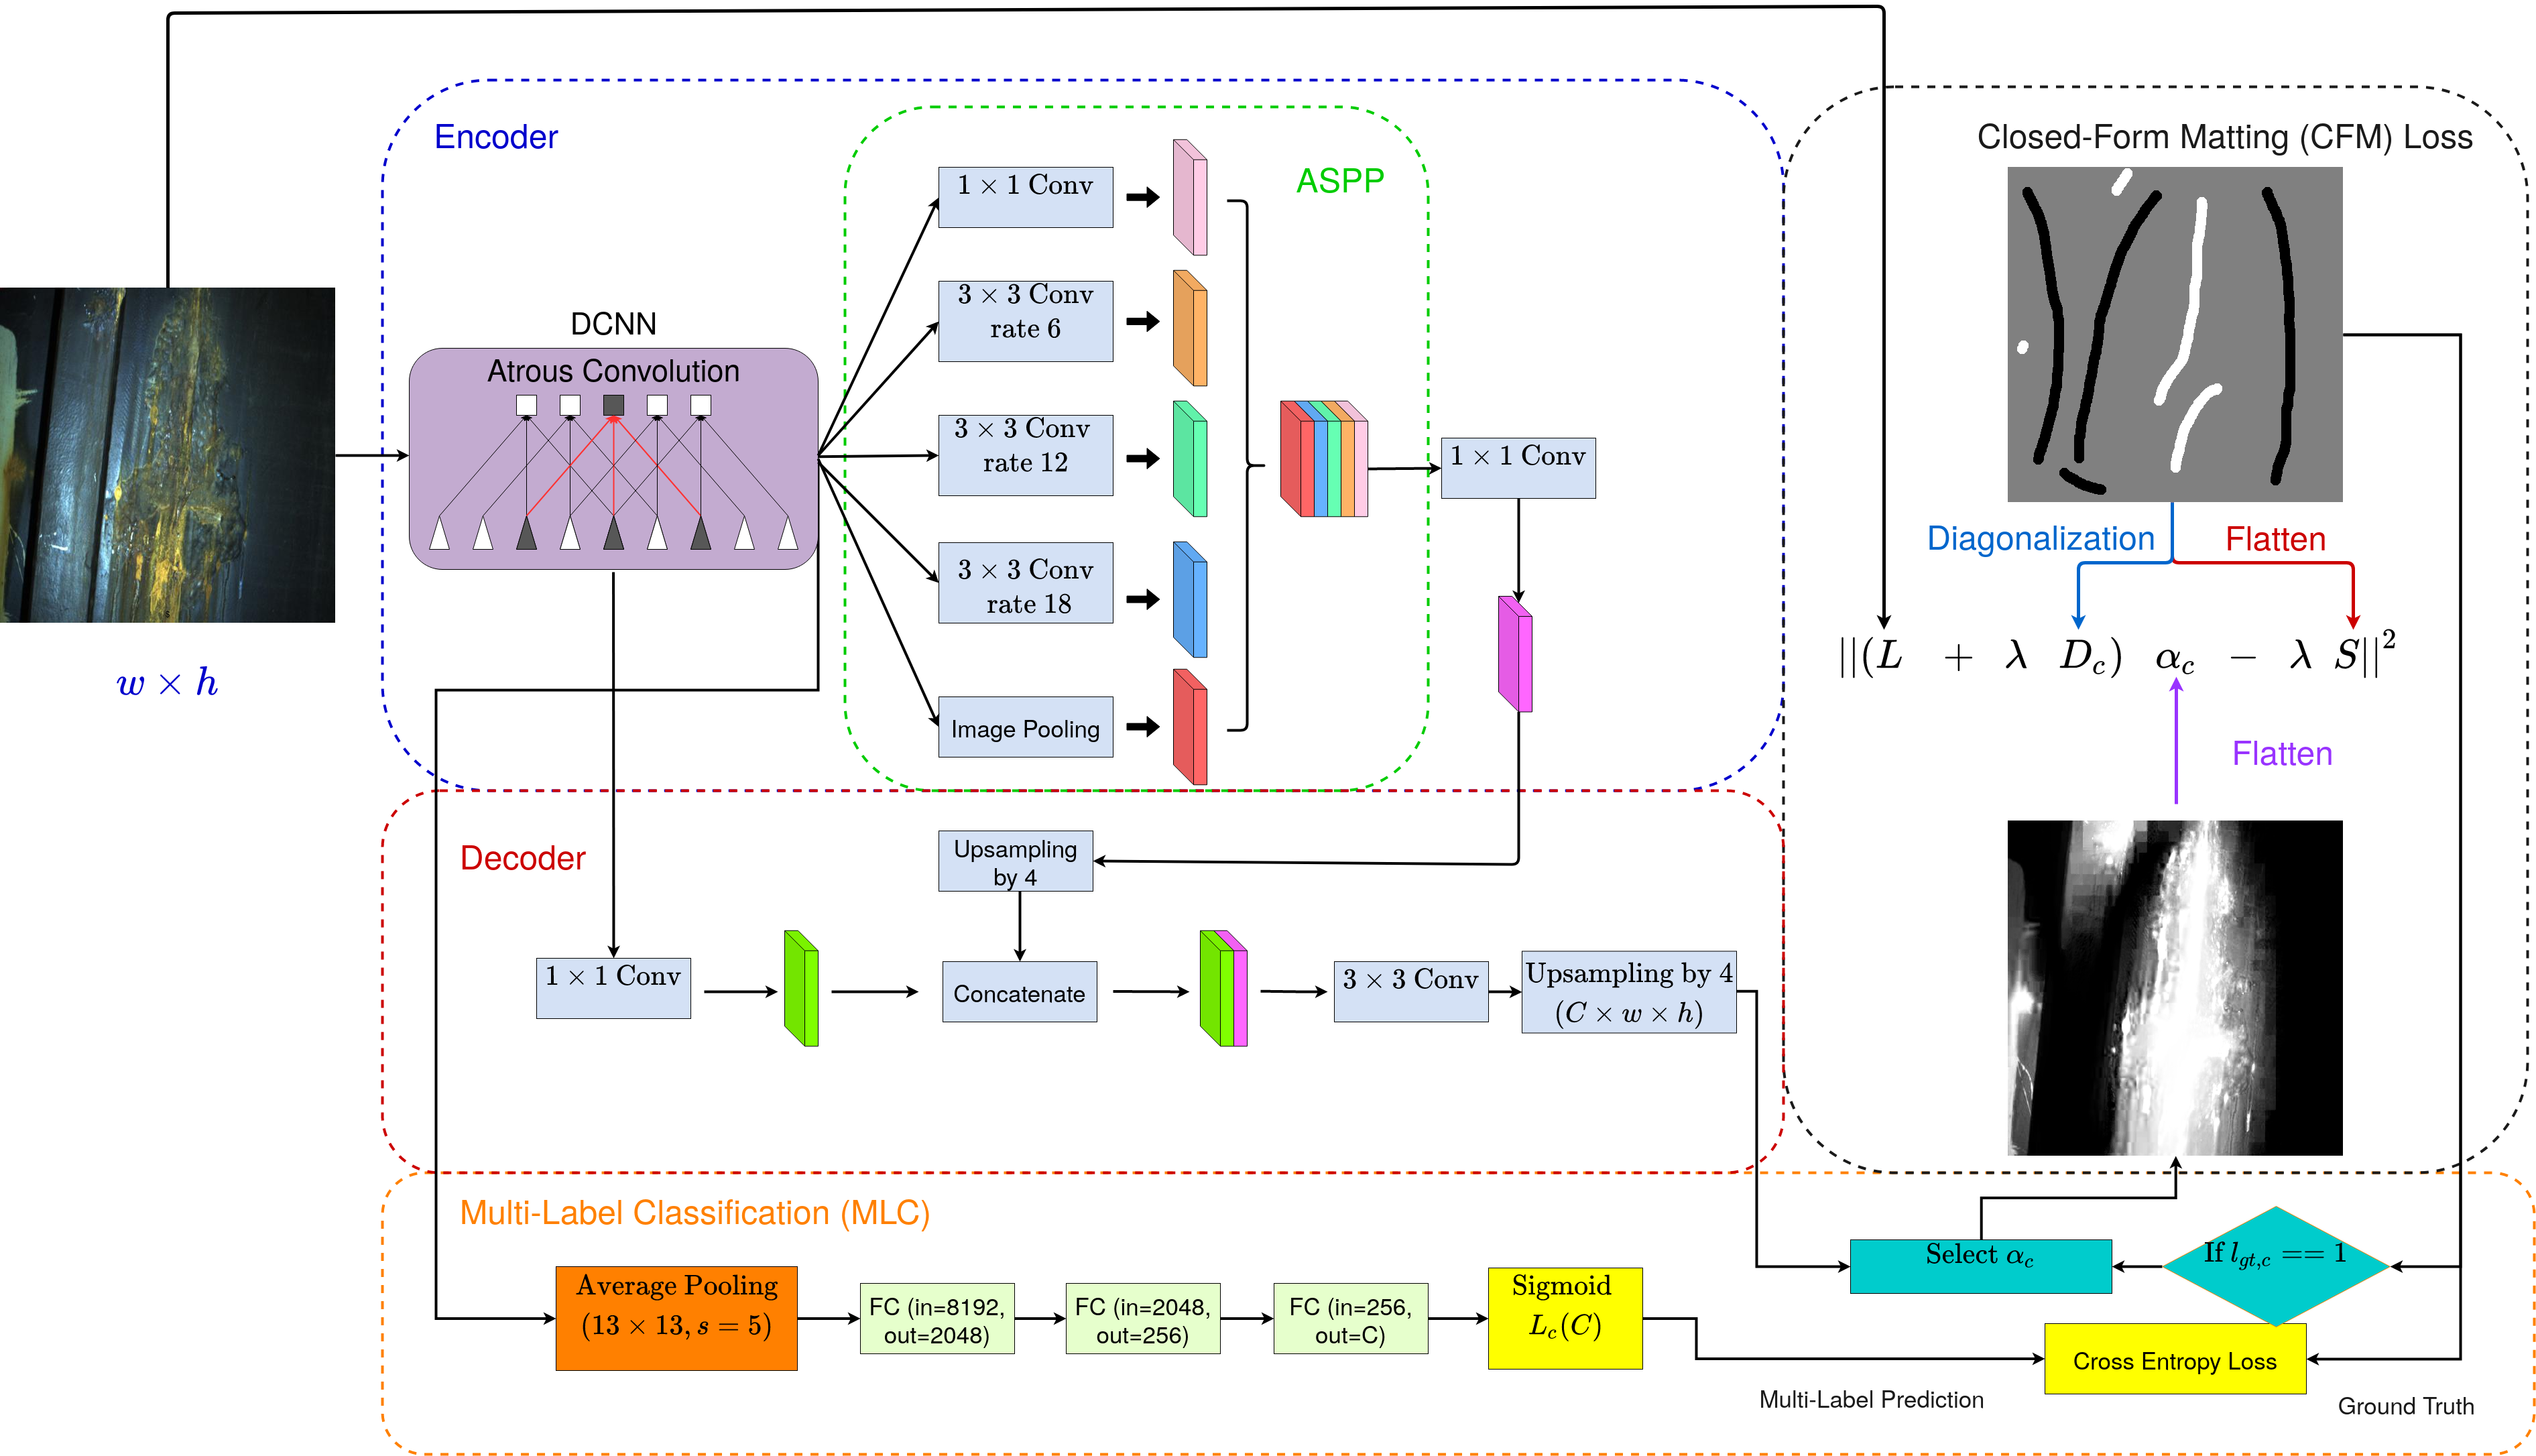
\includegraphics[width=1.8\columnwidth]{imgs/closed-form-segmentation.png}
    \caption{Training schematic diagram of DeepLabV3+ with the closed form loss. The encoder model is employed to extract multi-scale contextual information by using atrous convolution, then the ASPP model is used to integrate multi-scale information. A simple but effective decoder model is proposed to refine the segmentation results. The MLC model is connected to the encoder, which is used to obtain the category information of targets in the image. In the end, our CFM loss is used to train the network. }
    \label{fg:closed-form-loss-trianing}
\end{figure*}

\paragraph{Atrous Convolution}
The atrous convolution (dilated convolution) introduces a new parameter to the standard convolution called the "dilate rate", which is used to explicitly control the resolution of feature maps of DCNN. Compared to the standard convolution, the atrous convolution can obtain a larger receptive field, which can improve the segmentation performance and also increase the localization accuracy. On the other hand, the network can capture multi-scale contextual information by different dilated factors. Thus, the atrous convolution can provide the necessary information that is needed to improve the image segmentation performance \cite{papandreou2015modeling,chen2017deeplab}.

Considering two-dimensional inputs, for each location $i$ on the output $y$ and a filter $w$, atrous convolution is applied over the input feature map $x$ as in Eq. \ref{atrous_conv}.
\begin{equation}
    y\left[ i \right] = \sum\limits_{k} x \left[ i+r \cdot k \right]~w\left[ k \right]
    \label{atrous_conv}
\end{equation}
where the dilated rate $r$ directly affects the stride of convolution sampling. Furthermore, the standard convolution is considered as a special case, where $r=1$. Via changing the $r$ value, the receptive field of convolution can be changed adaptively. As shown in Fig. \ref{fg:atrous_conv}, using different dilated rate values in convolution operation, the receptive field changes significantly. Besides, stacking atrous convolution makes the receptive field growing exponentially in the DCNN model. 
\begin{figure}[t]
    \centering
    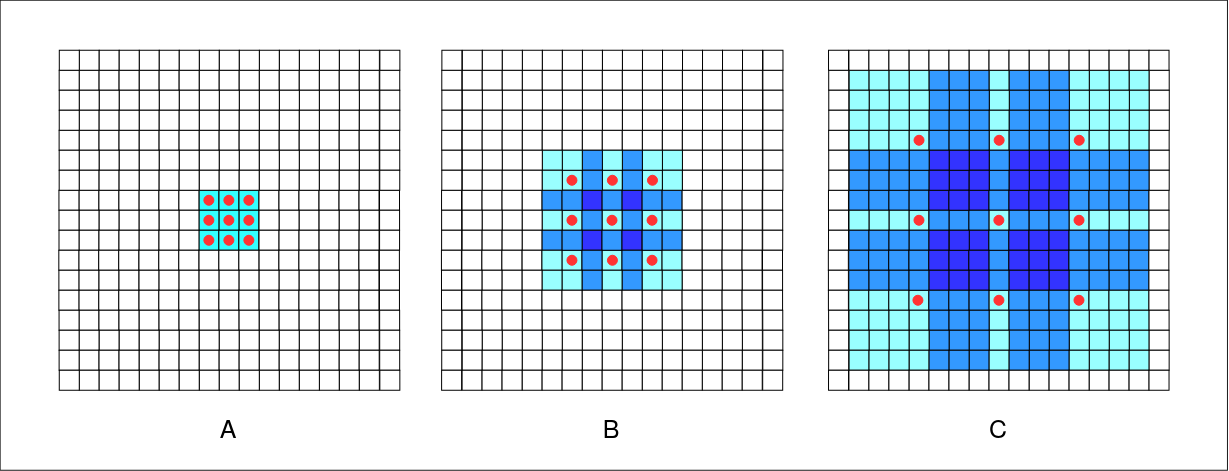
\includegraphics[width=\columnwidth]{imgs/atrous_conv.png}
    \caption{A diagrams illustration of the atrous convolution. In this figure. only 9 red points for a $3\times 3$ kernel are involved in the convolution operation, and other points in the receptive field are ignored. A is the standard convolution, where the $r$ is 1, its receptive field is only $3\times 3$; the $r$ in B is 2, and its receptive field is $7\times 7$; while C is the 4-dilated convolution, and its receptive field is $15\times 15$.}
    \label{fg:atrous_conv}
\end{figure}

\paragraph{Depthwise Separable Convolution}
The Depthwise Separable (DS) convolution \cite{chollet2017xception} is the combination of Depthwise and Pointwise convolution, which can drastically reduce computation complexity. Specifically, the DS convolution decomposes the standard convolution into Depthwise convolution, whose number of output channels equals the number of input channels, and then Pointwise convolution ($1\times 1$ convolution) is applied on the output of Depthwise convolution to obtain the target number of output channels. 
% \begin{figure*}[t]
%     \centering
%     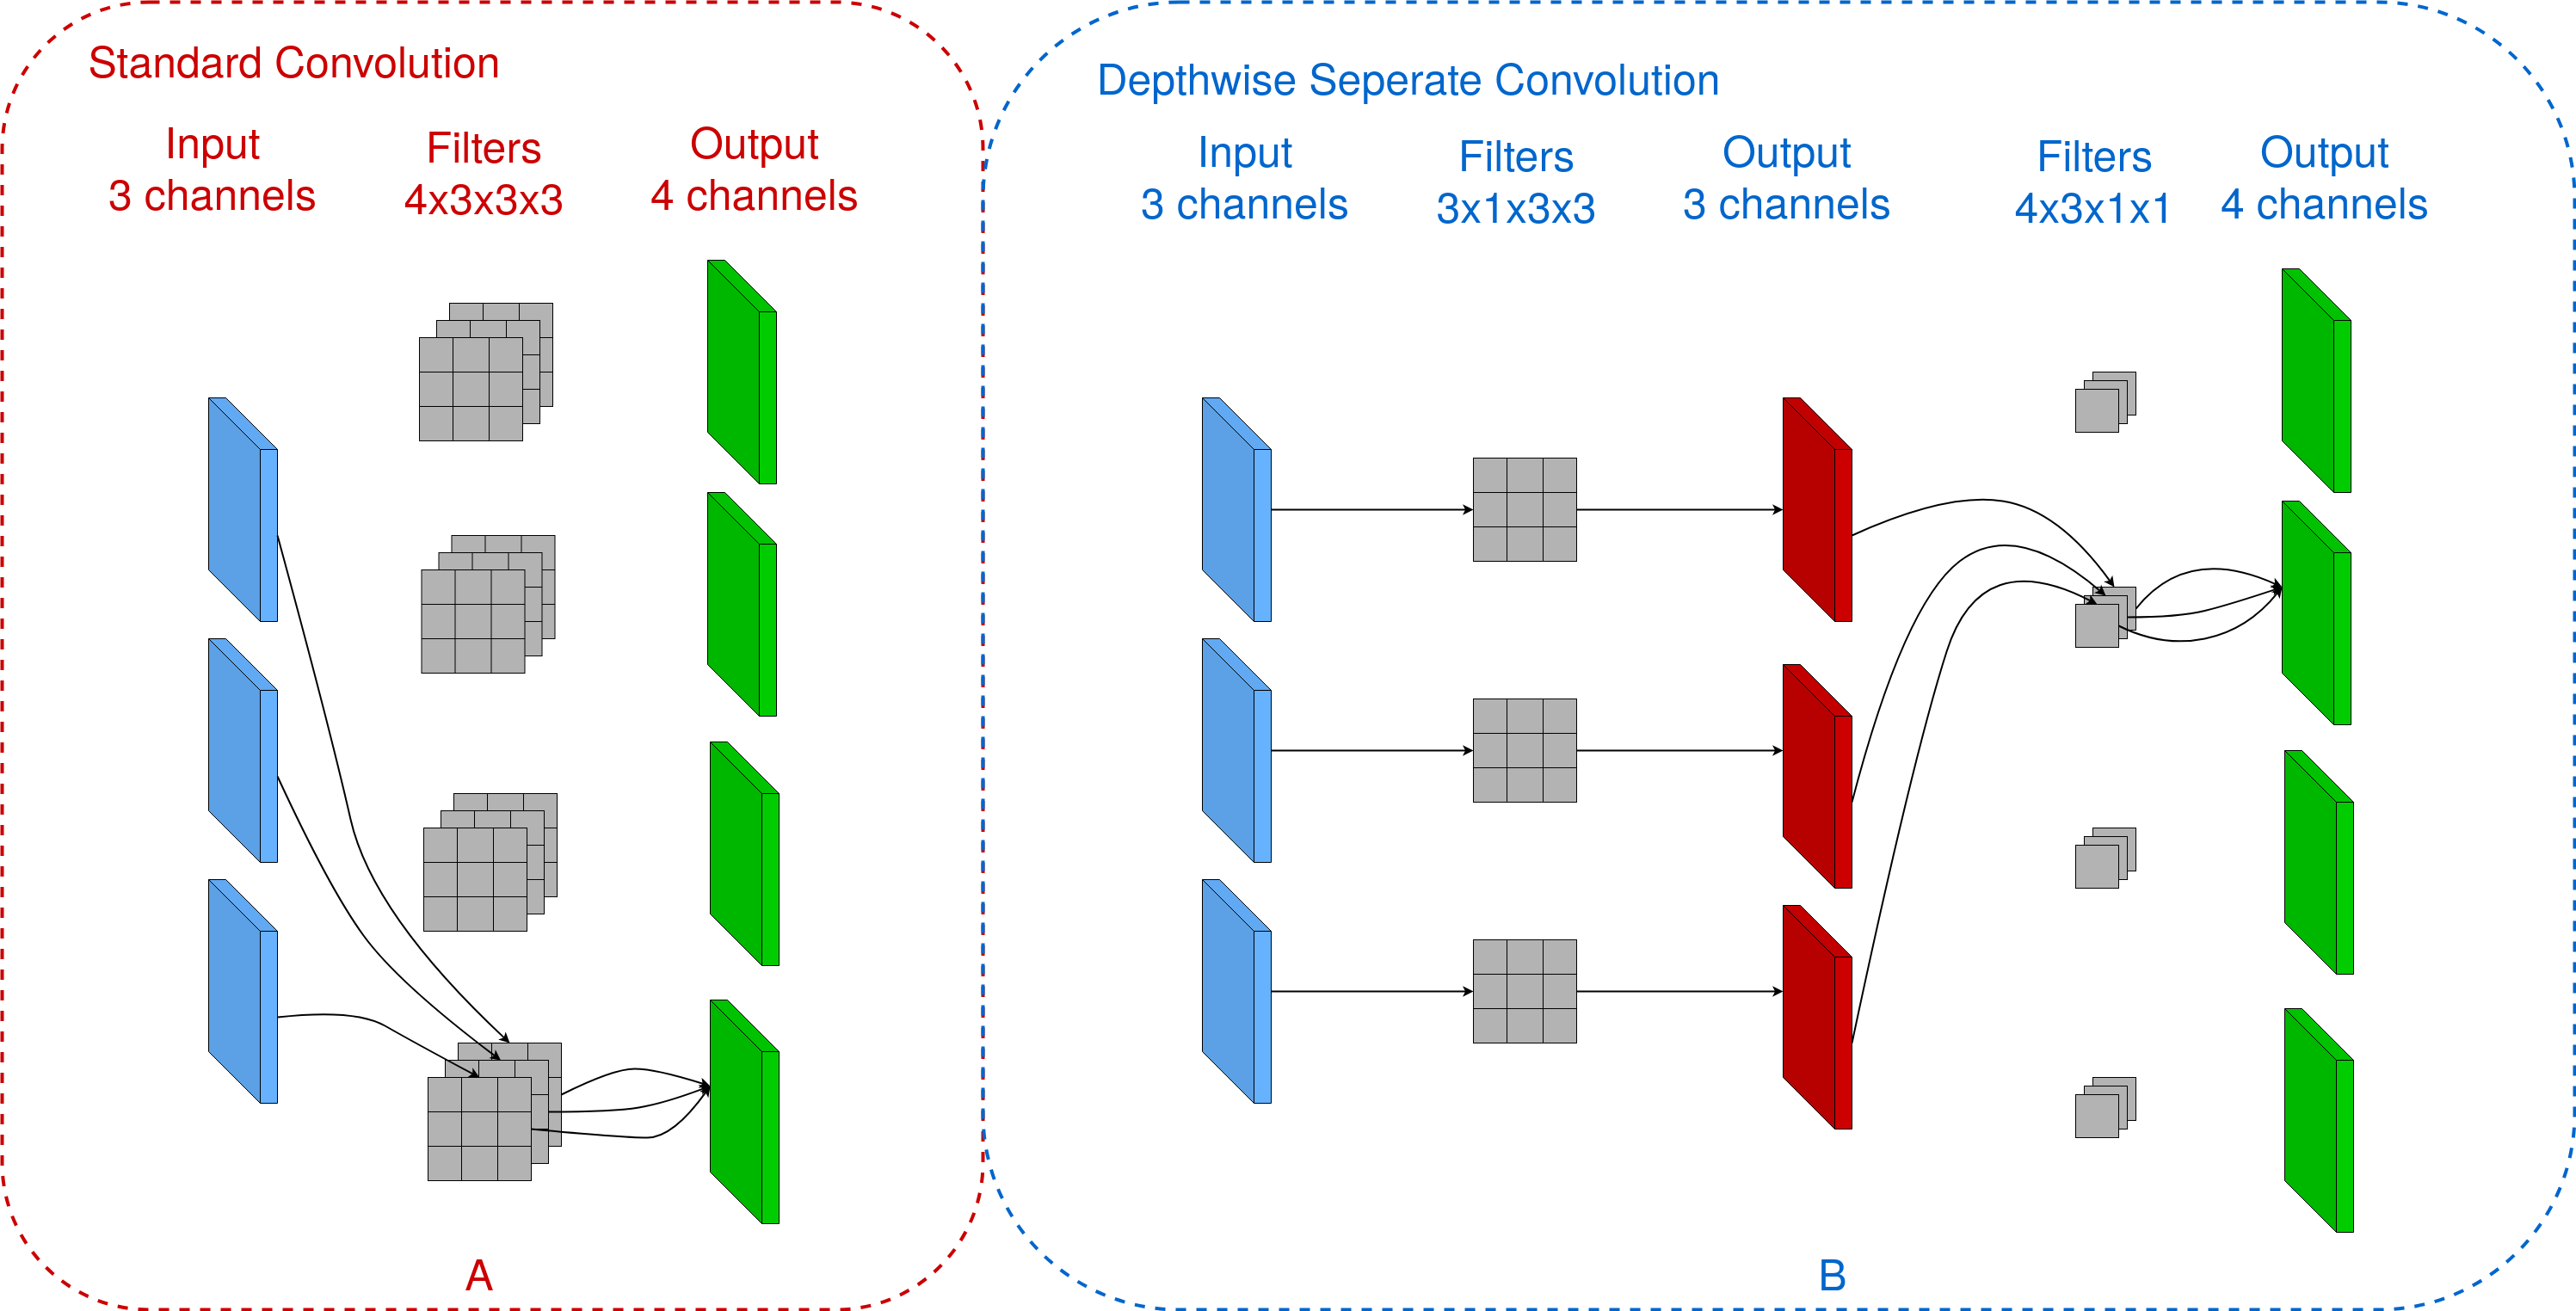
\includegraphics[width=1.6\columnwidth]{imgs/depthwise-seperate-convolution.png}
%     \caption{The comparison of standard convolution and depthwise separable convolution.}
%     \label{fg:ds_conv}
% \end{figure*}

% As can be observed in Fig. \ref{fg:ds_conv}, for instance, the number of parameters for standard convolution is 108 ($4\times 3\times 3\times 3$). While the number of parameters for depthwise convolution is 27 ($3\times 1\times 3\times 3$), and the number of parameters for pointwise convolution is 12 ($4\times 3\times 1\times 1$). At last, the number of parameters for DS convolution is 39 ($27+12$), which is almost a third of the standard convolution. Therefore, DS convolution contains fewer parameters and lower computation complexity in comparison with a standard convolution operation. Therefore, the fewer parameters, the less computation complexity, the faster computational speed.

In DeepLabV3+, the authors combine the atrous convolution with DS convolution, namely atrous separable convolution, and prove that atrous separable convolution significantly reduces the computation complexity of the proposed model while maintaining better performance \cite{chen2017rethinking}. 

\paragraph{Atrous Spatial Pyramid Pooling}
The Atrous Spatial Pyramid Pooling (ASPP) model is proposed in \cite{chen2017deeplab}, and it is inspired by spatial pyramid pooling \cite{lazebnik2006beyond,he2015spatial}, which can effectively improve the accuracy and efficiency for classifying regions of an arbitrary scale. The ASPP model in DeepLabV3+ applies three atrous convolutions with different atrous rates to capture multi-scale information. Besides, an average pooling and a $1\times 1$ convolution layer with 256 filters are applied on the input feature maps to obtain the image-level features. Therefore, the ASPP model consists of (a) a $1\times 1$ convolution and three $3\times 3$ convolutions with different dilated rates (6, 12, 18) and (b) a global average pooling. In the end, the resulting features from all branches are concatenated in the channel and pass through another $1\times 1$ convolution (256 filters and batch normalization). The architecture of the ASPP model can be seen in Fig. \ref{fg:closed-form-loss-trianing}. 

\paragraph{Encoder-Decoder Architecture}
The DeepLabV3+ is developed based on the DeepLabV3, taking advantage of atrous convolution to extract features of the DCNNs at arbitrary resolution and with a large receptive field, and to augment the ASPP model aimed at using multi-scale features by different dilated rates. The DeepLabV3 applies a naive decoder module, which bilinearly upsamples the features by a factor of 16. However, this work lacks the accuracy of the target's boundary in the semantic segmentation task. To address this problem, DeepLabV3+ proposes a simple but effective decoder module. As shown in Fig. \ref{fg:closed-form-loss-trianing}, the last feature maps of the encoder are upsampled by a factor of 4, and then concatenated with the corresponding low-level feature maps \cite{hariharan2015hypercolumns}. After, the output is obtained through a few $3\times 3$ convolutions to refine the feature maps, followed by another simple bilinear upsampling by a factor of 4. Herein, the proposed encoder-decoder structure is implemented to take the place of the single-applied decoder structure in \cite{chen2017rethinking} and improve the target boundary's segmentation performance. 
% and to improve the segmentation performance of the target boundary. 

\paragraph{Modified Aligned Xception}
The Xception model \cite{chollet2017xception}, which is employed as network backbone (denoted as X-65) in object detection \cite{qi2017deformable} and segmentation \cite{chen2018encoder} task, has been proved that it is useful to push the performance on the large scale dataset, such as MS-COCO \cite{lin2014microsoft}, PASCAL VOC 2012 \cite{everingham2012pascal}. Therefore, we also employ the Aligned Xception model in our work. 

Specifically, some changes based on \cite{qi2017deformable} need to be conducted, namely (1) similar to MRSA's work, the depth of Xception model is increased in this work apart from the structure of entry flow considering fast computation and memory efficiency; (2) all of the max-pooling layers in Xception model are replaced by depthwise separable convolution, where combines stride and dilated rate to obtain the arbitrary resolution feature maps; (3) the batch normalization and ReLU are used behind the $3\times 3$ depthwise convolution. 

% The architecture of the Modified Aligned Xception is shown in Fig. \ref{fg:xception}.
% \begin{figure*}[t]
%     \centering
%     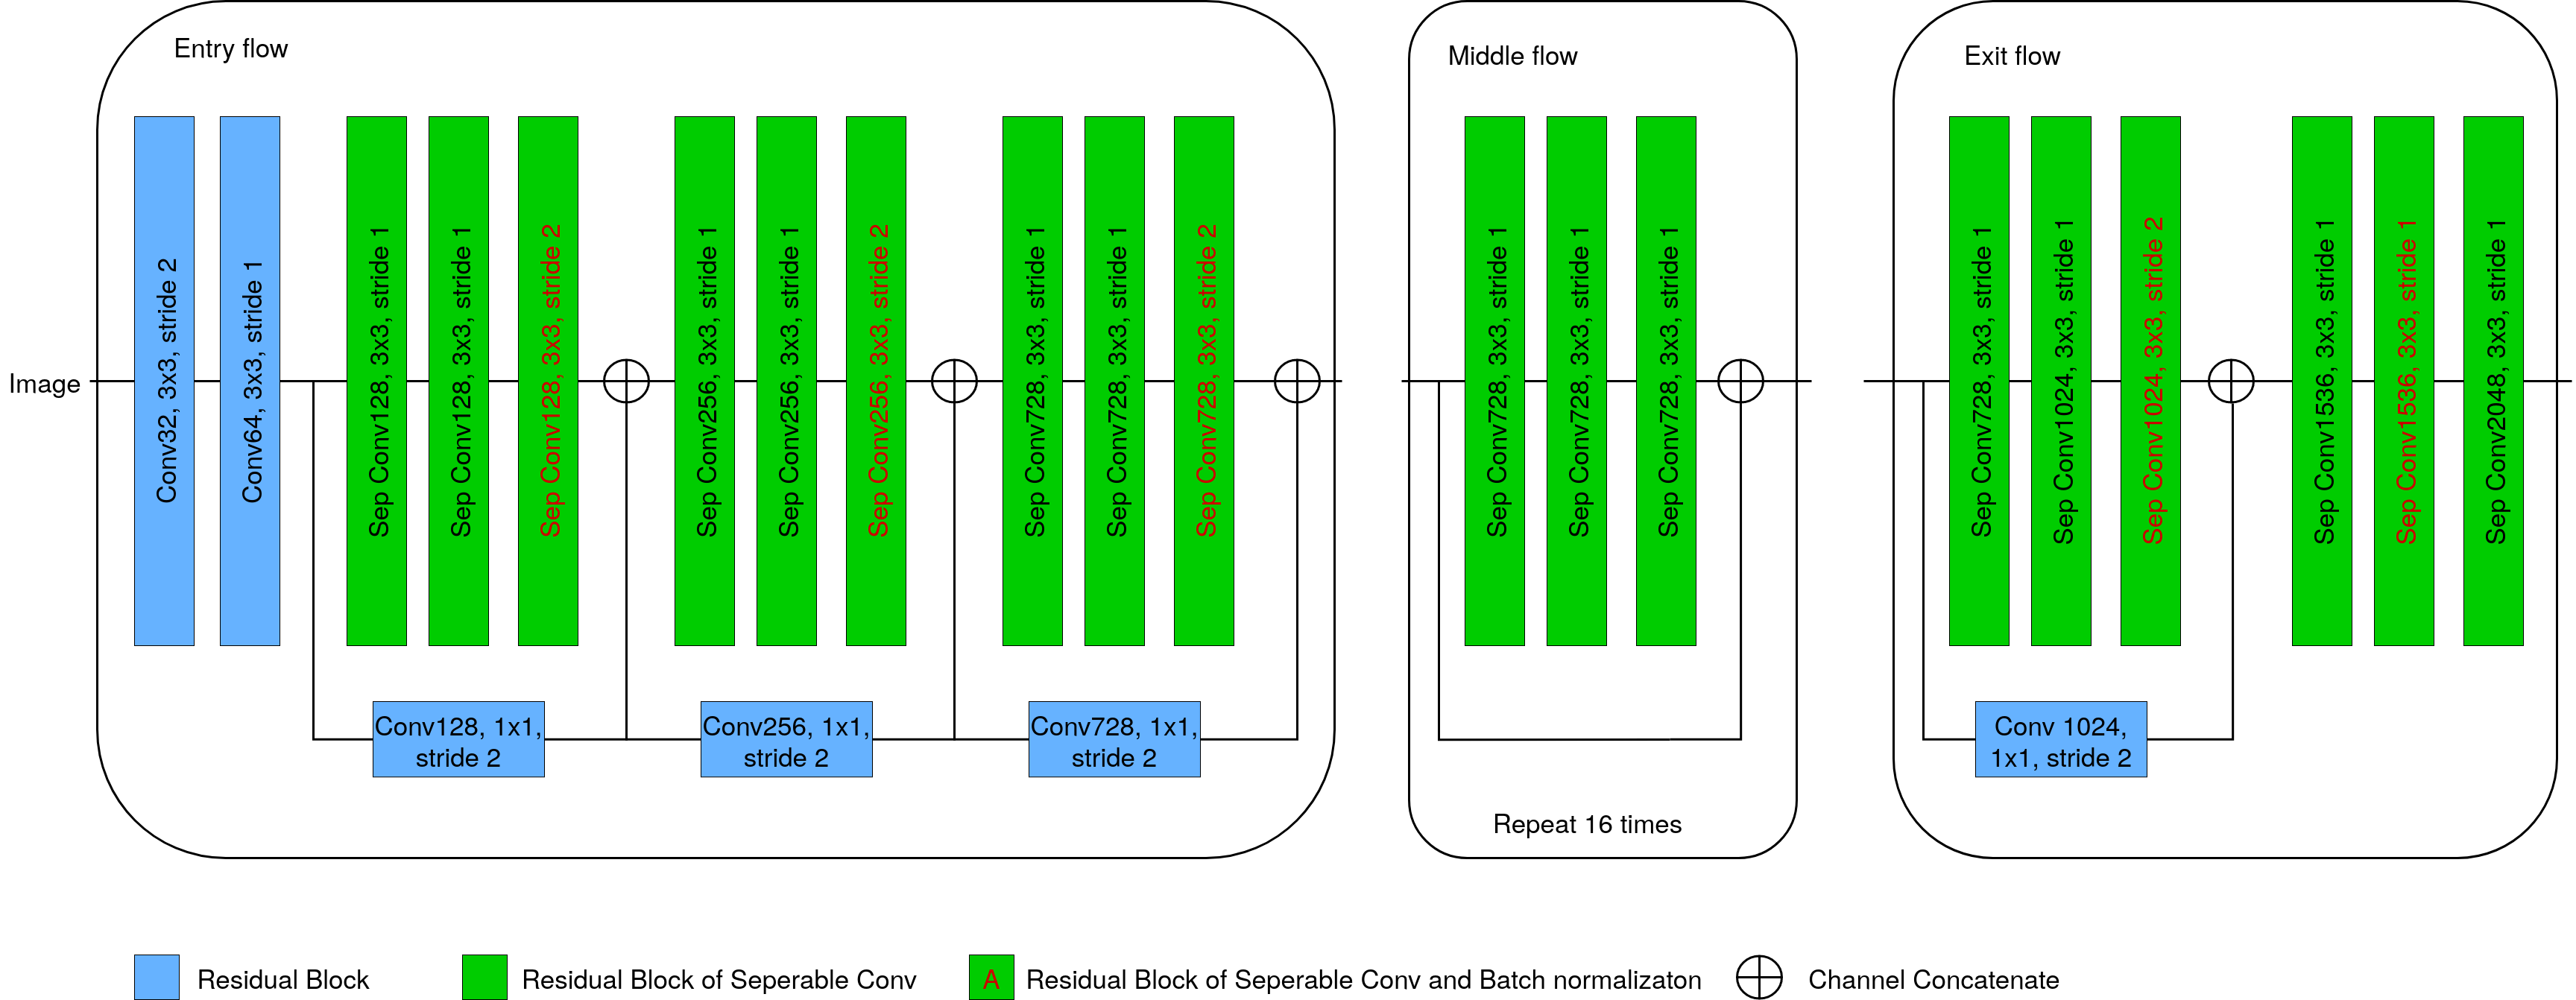
\includegraphics[width=1.8\columnwidth]{imgs/xception.png}
%     \caption{The architecture of Modified Aligned Xception. As can be observed, there are three major changes: a. more layers are added in the middle flow; b. the max pooling layer is replaced by the depthwise separable convolutions with stride; c extra batch normalization and ReLU are added after each $3\times 3$ depthwise convolution.}
%     \label{fg:xception}
% \end{figure*}

\subsubsection{U-Net}
The U-Net \cite{ronneberger2015u} is developed for BioMedical image segmentation, and its architecture is illustrated in Fig. \ref{fg:unet}. The U-Net consists of two paths. The first path is named as contraction path (also called the encoder), which is used to capture the context from the input image. The encoder is a stack of convolutional and pooling layers. The second path is the symmetric expanding path (also named the decoder) which is used to enable precise location combined with the feature maps of the encoder. Therefore, U-Net is an end-to-end fully convolutional network, and it achieves outstanding performance for medical image segmentation. 

\begin{figure*}[t]
    \centering
    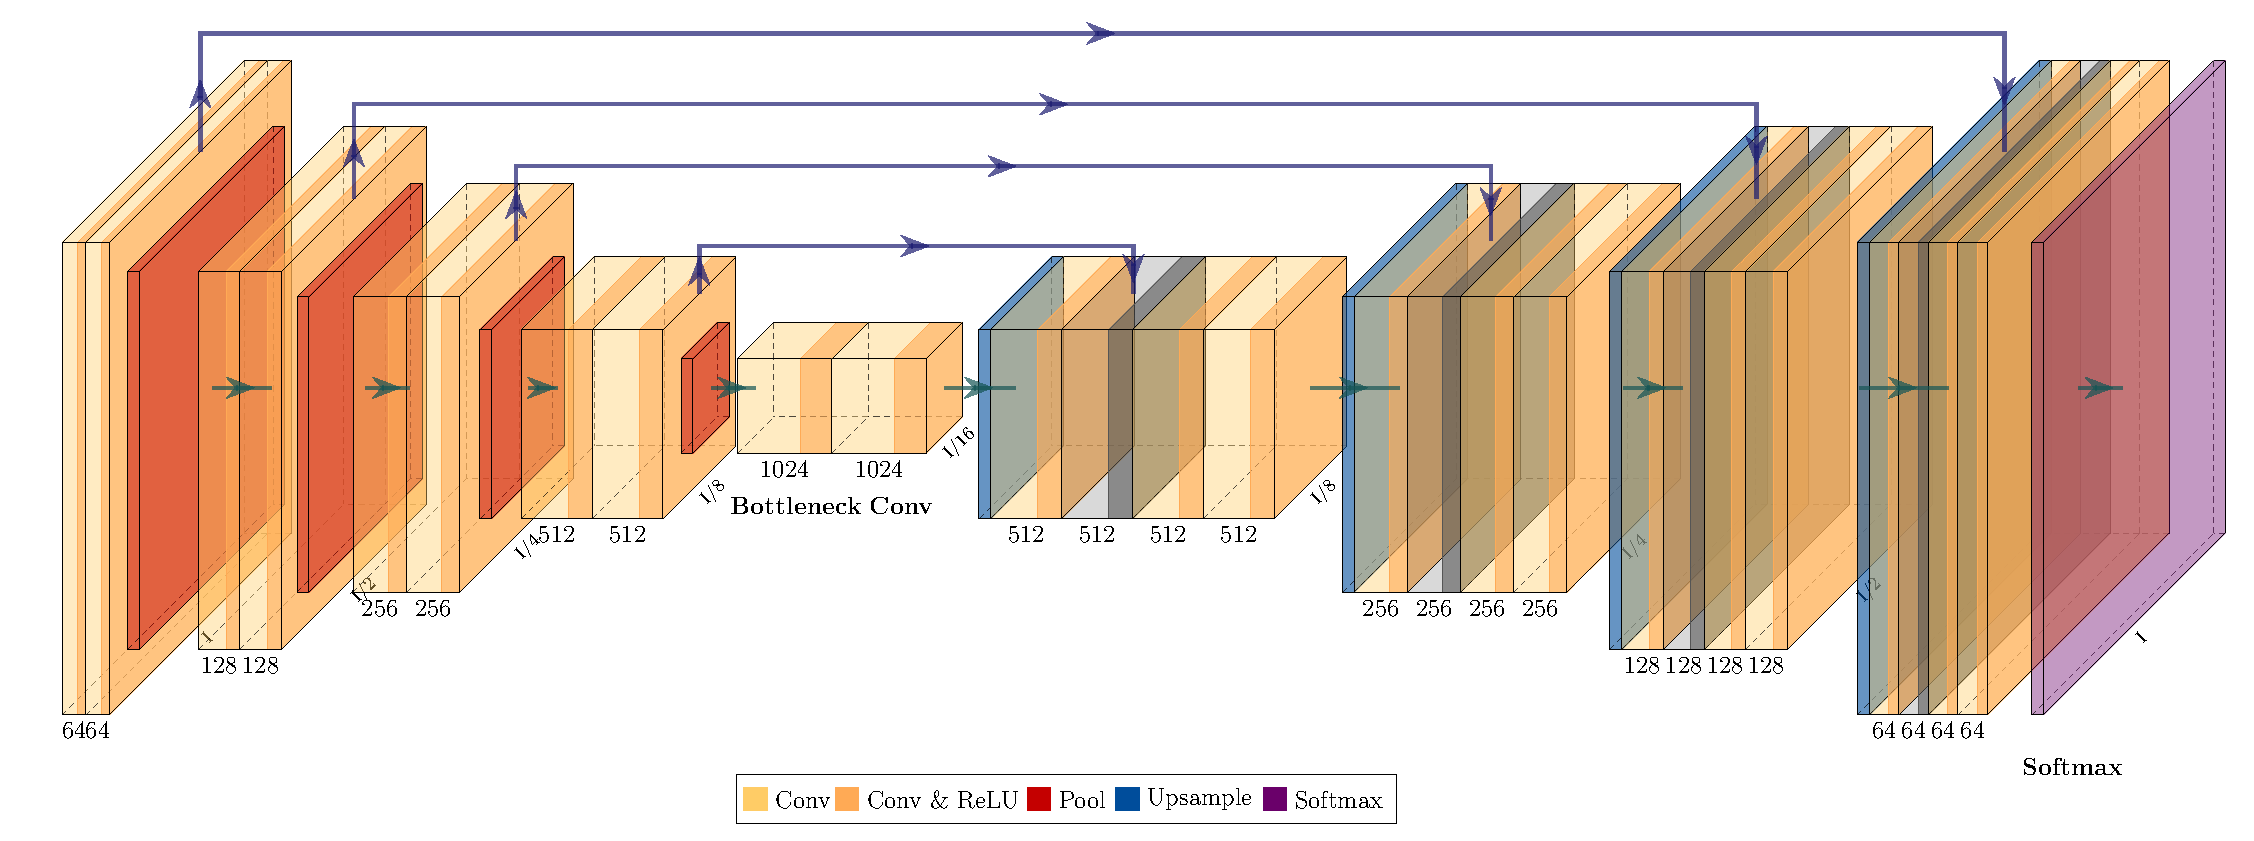
\includegraphics[width=1.8\columnwidth]{imgs/Unet.pdf}
    \caption{The architecture of U-Net. In this figure, \textit{Conv} represents convolutional layer with $3\times 3$ kernel; \textit{Conv~\&~ReLU} indicates convolutional layer connected with \textit{ReLU} activation; \textit{Pool} layer is used to decrease the dimension of the input feature; \textit{Upsample} is used to increase the dimension of the input feature; \textit{Softmax} activated function is used to get the segmentation for every category.  }
    \label{fg:unet}
\end{figure*}

\subsubsection{ERFNet}
ERFNet \cite{romera2017erfnet} is a lightweight segmentation network, which proposes a factorized residual (FR) layer to remain efficient while retaining remarkable segmentation performance. The residual layer \cite{he2016deep} has been proved that it can facilitate training and significantly reduce the performance degradation due to stacking a large number of convolutional layers. Specifically, the non-bottleneck in ResNets gains the accuracy for the increased depth network \cite{he2016deep,zagoruyko2016wide,rastegari2016xnor}. Inspired by the Non-bottleneck, a modified residual module is proposed using convolutions with 1D filters, namely non-bottleneck-1D module, as shown in Fig. \ref{fg:bottleneck}. By leveraging the decomposition in Fig. \ref{fg:bottleneck} [b], the non-bottleneck-1D can accelerate running time and reduce the parameters of the non-bottleneck module. 

\begin{figure}[t]
    \centering
    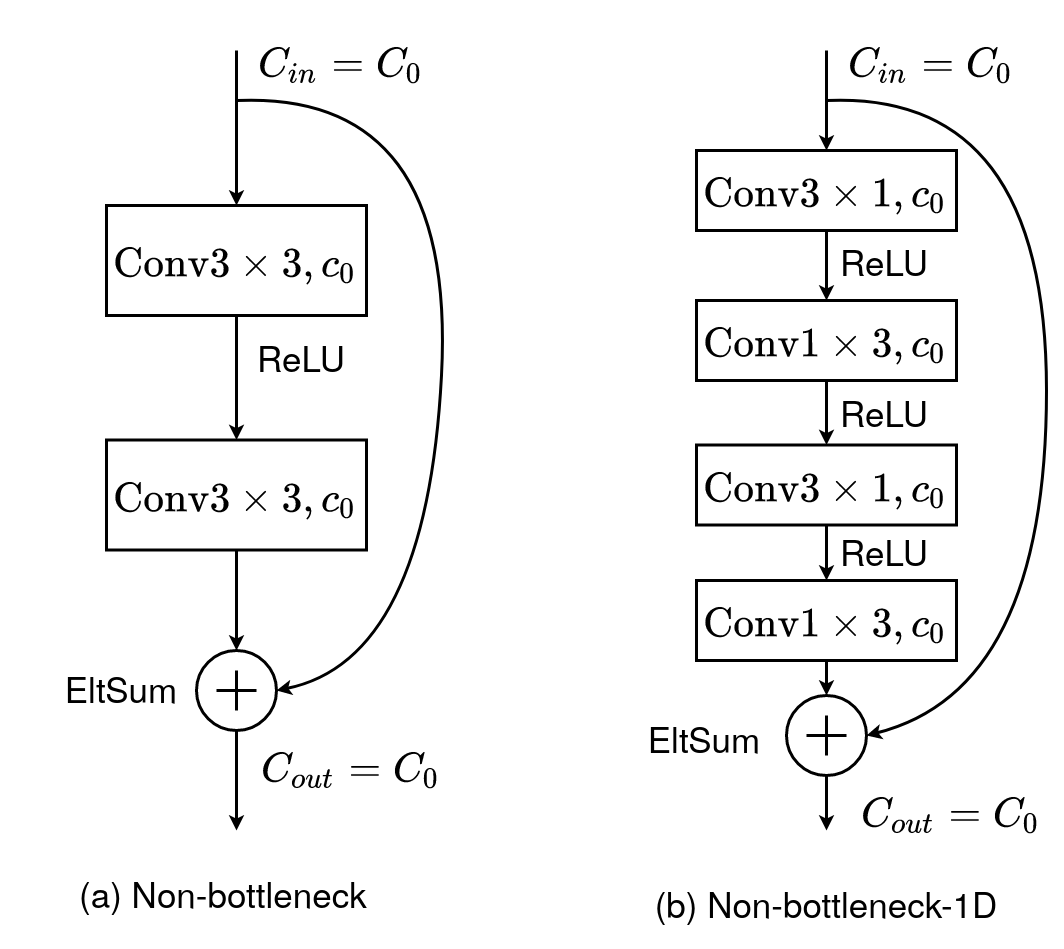
\includegraphics[width=0.8\columnwidth]{imgs/erf-non-bottleneck-1d.png}
    \caption{The illustration of (a) Non-bottleneck in \cite{he2016deep} and (b) Non-bottleneck-1D in \cite{romera2017erfnet}. In this figure, $C$ represents the channels of feature map. In the convolution block, ($d_{1} \times d_{2},~c$) indicates the kernel size ($d_1, d_2$) and the output channels ($c$) of feature maps. \textit{EltSum} denotes element-wise sum.  }
    \label{fg:bottleneck}
\end{figure}

The architecture of ERFNet follows a prevail encoder-decoder structure. Inspired by ENet \cite{paszke2016enet}, a complicated but efficient encoder is designed to gather context from the input image. Particularly, every down-sample block of ERFNet performs down-sampling by concatenating outputs of a convolutional layer using $3\times 3$ kernels with stride 2, and a max-pooling layer. After down-sampling, some non-bottleneck-1D modules with different dilated rates \cite{yu2015multi} are applied to improve the segmentation performance. Similar to the design of ENet, a simple decoder is used to up-sample the encoder's output to match the input resolution. For every up-sample block, a deconvolution layer with stride 2 is adopted. The architecture of ERFNet is fully depicted as in Table \ref{tab:erf_arch}.

\begin{table}[t]
    \centering
    \caption{A detailed demonstration for the architecture of ERFNet. \textit{OUT-C} represents the output channels, \textit{OUT-DIM} indicates the dimension of output feature maps, and \textit{C} denotes the number of category. }
    \label{tab:erf_arch}
    % \begin{tabular}{p{0.5cm}|p{4.5cm}|p{1cm}|p{1.5cm}}
    \begin{tabular}{p{0.5cm}p{4.5cm}p{1cm}p{1.5cm}}
        \toprule %\toprule
         & \textbf{Type} & \textbf{OUT-C} & \textbf{OUT-DIM} \\
        \midrule %\midrule
        \multirow{12}{0.5cm}{\rotatebox[origin=c]{90}{Encoder}}
        & down-sample block                   & 16           & $512\times 256$        \\
        \cmidrule{2-4}
        & down-sample block                   & 64           & $256\times 128$        \\
        & 5$\times$ non-bottleneck-1D         & 64           & $256\times 128$        \\
        \cmidrule{2-4}
        & down-sample block                   & 128          & $128\times 64$         \\
        & non-bottleneck-1D (dilated 2)       & 128          & $128\times 64$         \\
        & non-bottleneck-1D (dilated 4)       & 128          & $128\times 64$         \\
        & non-bottleneck-1D (dilated 8)       & 128          & $128\times 64$         \\
        & non-bottleneck-1D (dilated 16)      & 128          & $128\times 64$         \\
        & non-bottleneck-1D (dilated 2)       & 128          & $128\times 64$         \\
        & non-bottleneck-1D (dilated 4)       & 128          & $128\times 64$         \\
        & non-bottleneck-1D (dilated 8)       & 128          & $128\times 64$         \\
        & non-bottleneck-1D (dilated 16)      & 128          & $128\times 64$         \\
        \midrule
        \multirow{5}{0.5cm}{\rotatebox[origin=c]{90}{Decoder}}
        & up-sample block                     & 64           & $256\times 128$        \\
        & 2$\times$ non-bottleneck-1D         & 64           & $256\times 128$        \\
        \cmidrule{2-4}
        & up-sample block                     & 16           & $512\times 256$        \\
        & 2$\times$ non-bottleneck-1D         & 16           & $512\times 256$        \\
        \cmidrule{2-4}
        & up-sample block                     & C            & $1024\times 512$       \\
        \bottomrule
    \end{tabular}
\end{table}


\section{Experiments and Discussion}
\label{exp_dis}
In this section, we conduct experiments and illustrate the performance of our approach on our two inspection tasks and two MCSS tasks. In Section \ref{sec:exp_setup}, the experimental environments, including the dataset, the evaluated metrics, and the hyper-parameters of experiments, are introduced. Then, we evaluate the matting performance for the inspection tasks in Section \ref{sec:matting_eval_ins}, and the segmentation performance for inspection tasks is illustrated in Section \ref{sec:seg_performance_ins}. For the MCSS tasks, the segmentation performance is compared in Section \ref{sec:seg_performance_mcss}. In the end, some examples of segmentation results for our two tasks are shown in Section \ref{sec:vis_exp_results}.

\subsection{Experiment Settings}
\label{sec:exp_setup}
\paragraph{Datasets}The dataset from the COR task consists of 241 images in total, three-fourths of which are designated for training and the rest for testing. Regarding the dataset of the BIO task, it contains 195 images, and the same strategy is adopted for splitting into the training and validation sets. Both datasets are obtained from real industry scenes. During training, an online data augmentation strategy, including rotation, scaling, and random cropping, is used to increase the diversity of our training dataset. 

In order to verify the effectiveness of our solution for the MCSS task, two subsets are extracted from Pascal VOC 2012 and CityScapes, respectively. The VOC subset consists of 453 images and has 6 categories, which are plane, bike, person, car, dog, and cat, while the CityScape subset contains 450 images with 9 categories (road, building, sidewalk, traffic sign, plant, sky, person, car, and bike). For both datasets, we select 400 images to train the network, and the rest is used for validation. 

To obtain the scribble annotations, a color brush is used to partially mark the pixels of target and background, as shown in Fig. \ref{fg:weak-annotations}. Other pixels, whose grayscale values are 128, represent unknown, which need the network to learn its label and propagate the information from labelled pixels. 

\paragraph{Implementation Details}
All experiments have been implemented using the Pytorch framework running in a PC fitted with an NVIDIA GeForce RTX 2080 Ti GPU, a 2.9 GHz 12-core CPU with 32 GB RAM, and Ubuntu 64-bit. For experiments using the DeepLabV3+ model, we adopt the same training details for three different backbones (ResNet101, Xception, and MobileNet), i.e., initializing the backbones using the ImageNet \cite{russakovsky2015imagenet} pre-trained model, resizing the input images to $513\times 513$ dimensions for the inspection tasks and $321 \times 321$ for the MCSS tasks, optimizing the network via the Adam algorithm, setting the initial learning rate as 0.001. In the case of U-Net as the segmentation backbone, we resize the input images to $512\times 512$ dimensions, while the input images are resized to $320\times 160$ in the case of ERFNet. Regarding $\lambda$ in (\ref{mseloss_closed_form}), we set it as 100, which is the same as in \cite{levin2007closed}. 

\paragraph{Evaluation Metrics}
For quantitative evaluation of our approach, we evaluate the performance of our approach in two aspects: a. the accuracy of the closed-form solution; b. the image segmentation performance. 

As mentioned in section \ref{subsec:closed-form-loss}, our approach essentially uses a neural network to obtain the approximate closed-form solution of a sparse linear system. Therefore, we use three metrics to evaluate our approach. Regarding the Matte ground truth, we select the results of the CFM approach. The metrics are explained in the following.
% Namely the sum of absolute differences (SAD) and mean square error (MSE). The calculation method of these metrics is as follow.
\begin{itemize}
    \item The mean Absolute Differences (mAD) can be formally stated as follows: give the alpha of our approach $\alpha_i$ for a total of N pixels, and the solution of Closed-Form Matting (CFM) approach $\alpha^*_i$, it is defined as Eq. \ref{eq:metric_sad}.
    \begin{equation}
        \text{mAD} = \frac{\sum\limits_{i\in N}|\alpha_i - \alpha^*_i |}{N}
        \label{eq:metric_sad}
    \end{equation}

    The Mean Square Error (MSE) is to compute the mean Euclidean distance between the predicted $\alpha_i$ and the solution of CFM approach $\alpha^*_i$. It can be expressed as follows. \\
    \begin{equation}
        \text{MSE} = \frac{\sum\limits_{i\in N} (\alpha_i - \alpha^*_i)^2}{N}
        \label{eq:metric_mse}
    \end{equation}
    \item The Gradient Error (GE) is to calculate the gradient difference between the alpha matte $\alpha_i$ and the output $\alpha^*_i$ of the CFM approach, which is defined in Eq. \ref{eq:metric_ge}. Here, $\nabla$ means the gradient, which can be obtained by convolution operation using a first-order Gaussian derivative filter. $q$ is a hyper-parameter, and it is set to 2 in our experiments.  
    \begin{equation}
      \text{GE} = \sum\limits_{i\in N} (\nabla \alpha_i - \nabla \alpha^*_i)^q
      \label{eq:metric_ge}
    \end{equation}
\end{itemize}

To obtain the segmentation mask from the matting results, four thresholds (0.4, 0.5, 0.6, 0.7) are set for the matting results $\alpha$. Specifically, the segmentation results of category $c$ ($p_{seg,c}$) are obtained as follows,\
\begin{equation}
    % \begin{aligned}
    p_{seg,c} = 
    \begin{cases}
        1,~~~\alpha \geq \gamma \\
        0,~~~\alpha < \gamma 
    \end{cases} 
    \gamma \in \left[0.4, 0.5, 0.6, 0.7 \right]
    % \end{aligned}
    \label{eq:obtain_seg}
\end{equation}

In order to evaluate the performance of segmentation, some common metrics are considered, including:
\begin{itemize}
    \item The Intersection Over Union (IOU) is to compute the ratio of intersection and union between the prediction and ground truth. Formally, let $n_{ij}$ be the number of pixels of class $i$ fall into class $j$, the IOU is defined as in Eq. \ref{eq:metric_miou},
    \begin{equation}
        \text{IOU} = \sum\limits_{i}\frac{n_{ii}}{\sum\limits_{j} n_{ij} + \sum\limits_{j}n_{ji} - n_{ii}}
        \label{eq:metric_miou}
    \end{equation}

    \item The Recall (Rec) and Precision (Prec) also are computed to evaluate the performance of our approach, which can be expressed as follows:
    \begin{equation}
        \begin{aligned}
        \text{Rec} &= \sum\limits_{i} \frac{TP_i}{TP_i + FN_i}  = \sum\limits_{i} \frac{TP_i}{T_i} \\
        \text{Prev} &= \sum\limits_{i} \frac{TP_i}{TP_i + FP_i}  = \sum\limits_{i} \frac{TP_i}{P_i}
        \end{aligned}
        \label{eq:metric_rec_prev}
    \end{equation}
    where $TP_i$, $FP_i$ and $FN_i$ are respectively the true positives, false positives and false negatives for class $i$ and $T_i$ and $P_i$ are, respectively, the number of positives in the ground truth and the number of predicted positives, both for class $i$. 

    \item the F1 score is used as the the harmonic mean of precision and recall:
    \begin{equation}
        \text{F1} = \frac{2 \cdot \text{mPrec} \cdot \text{mRec}}{\text{mPrec} + \text{mRec}}
        \label{eq:metric_f1}
    \end{equation}
\end{itemize}

% To compare the segmentation performance of our approach and CFM approach, the segmentation results of CFM approach are set as the ground truth and the segmentation results of our approach are set as the prediction. Thus, the IOU, mRec, mPrec, and $\text{F}_1$ are computed to evaluate the performance of our approach. 

In the case of the COR task, we make use of fully supervised masks/ground truth in order to be able to report accurate segmentation metrics. This ground truth has been manually generated only for this purpose. Regarding the BIO task, since the photos are taken in the underwater environment, it is difficult and expensive to obtain the fully supervised pixel-wise ground truth. Therefore, we obtain the ground truth from the matting results of the CFM approach by setting thresholds, which is only for the purpose of evaluation. 

Regarding the MCSS tasks, the IOU is obtained for every category. Then the mIOU is attained by mean of every category IOU value. 
% Then the mIOU is used to evaluate the segmentation performance, which is the mean of every category IOU value.

\subsection{Evaluation for Matting Performance}
\label{sec:matting_eval_ins}
Compared to the CFM algorithm, our approach implements the same loss function. Differently, a segmentation network is used to obtain the closed-form solution. Therefore, our approach eliminates redundant iterative optimized procedures. In this section, variants of segmentation networks are trained and compared with the results of the CFM algorithm. 

There are already many image segmentation networks, which have achieved good segmentation performance. In this work, we select to use DeepLabV3+ \cite{chen2018encoder}, U-Net \cite{ronneberger2015u}, which obtains excellent segmentation performance for natural and medical images, and ERFNet \cite{romera2017erfnet}, which applies a small scale network to obtain good segmentation performance for the CityScape benchmark \cite{cordts2016cityscapes}. 

We respectively select one example from our two inspection tasks to compare the values of solution in Fig. \ref{fg:compare_matting_figure}. Comparing the distribution of the solutions from different segmentation networks, it can be seen that different solutions' distributions have similar a shape. Especially for the COR task (the second row in Fig. \ref{fg:compare_matting_figure}), using DeepLabV3+ with Xception backbone can obtain additional mattes, which have a similar character to corrosion. In our case, these additional mattes can be seen as suspicious targets.

\begin{figure*}[t]
    \centering
    \begin{tabular}{@{\hspace{0mm}}c@{\hspace{0.5mm}}c@{\hspace{0.5mm}}c@{\hspace{0.5mm}}c@{\hspace{0.5mm}}c@{\hspace{0.5mm}}c@{\hspace{0.5mm}}c@{\hspace{0mm}}}
        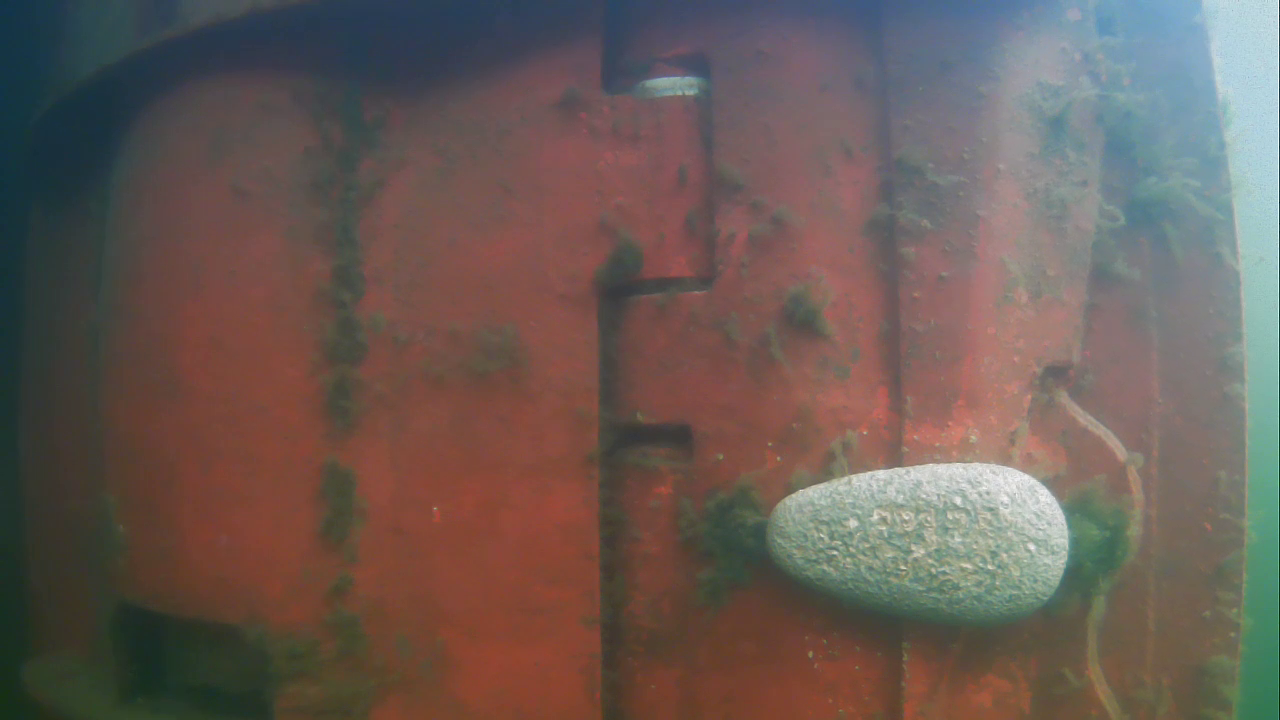
\includegraphics[width=0.25\columnwidth,  height=0.25\columnwidth]{imgs/beye_01_000900.png} &
        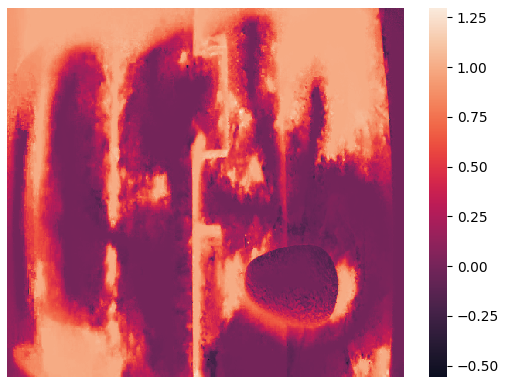
\includegraphics[width=0.3\columnwidth,   height=0.25\columnwidth]{imgs/hm_bio_cfm.png} &
        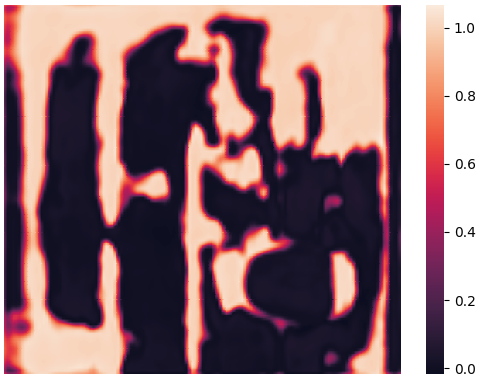
\includegraphics[width=0.3\columnwidth,   height=0.25\columnwidth]{imgs/hm_bio_res101.png} &
        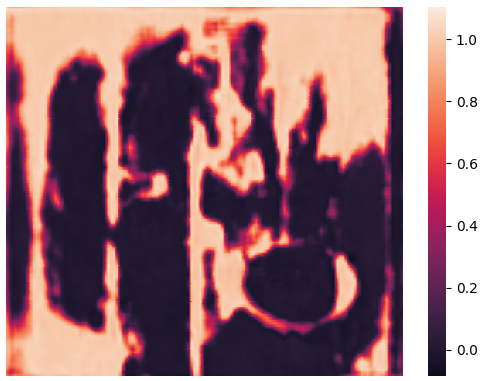
\includegraphics[width=0.3\columnwidth,   height=0.25\columnwidth]{imgs/hm_bio_xception.png} &
        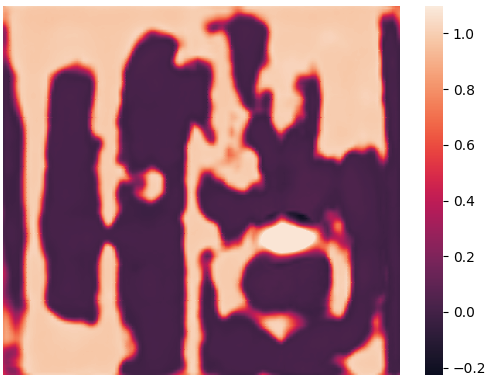
\includegraphics[width=0.3\columnwidth,   height=0.25\columnwidth]{imgs/hm_bio_mobilenet.png} &
        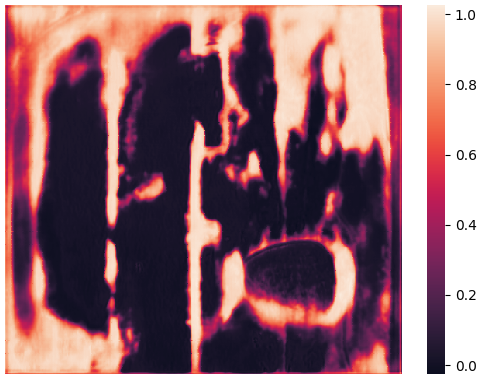
\includegraphics[width=0.3\columnwidth,   height=0.25\columnwidth]{imgs/hm_bio_unet.png} &
        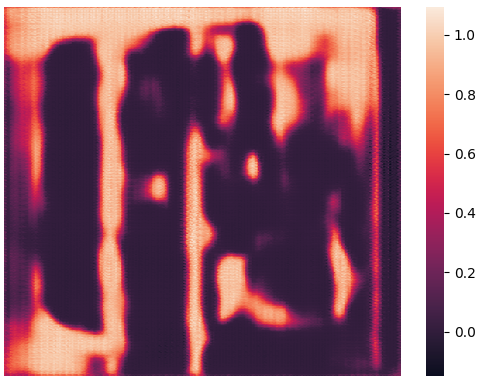
\includegraphics[width=0.3\columnwidth,   height=0.25\columnwidth]{imgs/hm_bio_erf.png} \\

        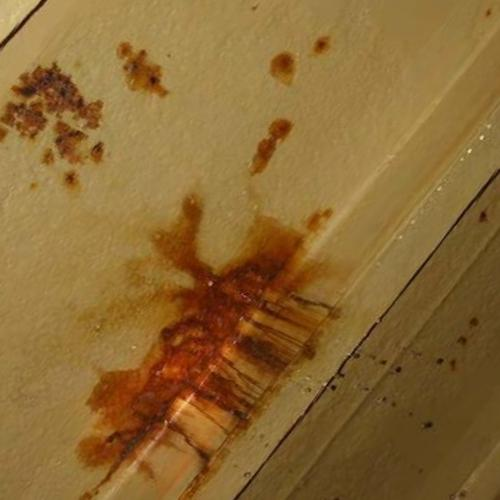
\includegraphics[width=0.25\columnwidth,  height=0.25\columnwidth]{imgs/image072_60.jpg}  &
        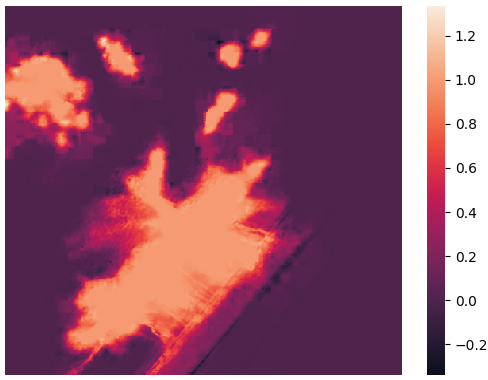
\includegraphics[width=0.3\columnwidth,   height=0.25\columnwidth]{imgs/hm_corrosion_cfm.png} &
        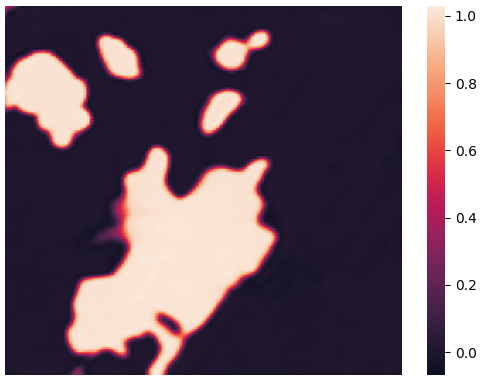
\includegraphics[width=0.3\columnwidth,   height=0.25\columnwidth]{imgs/hm_corrosion_res101.png} &
        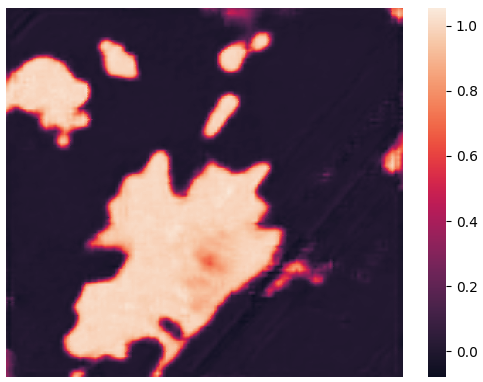
\includegraphics[width=0.3\columnwidth,   height=0.25\columnwidth]{imgs/hm_corrosion_xception.png} &
        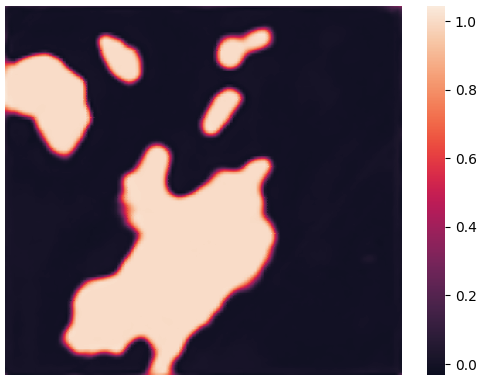
\includegraphics[width=0.3\columnwidth,   height=0.25\columnwidth]{imgs/hm_corrosion_mobilenet.png} &
        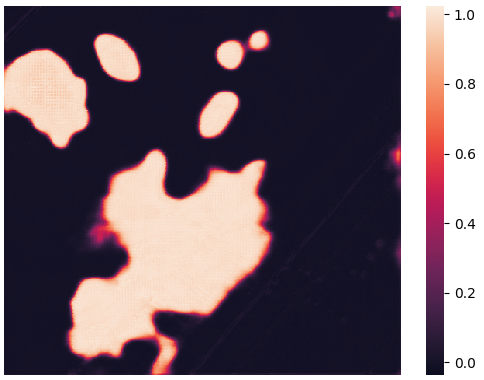
\includegraphics[width=0.3\columnwidth,   height=0.25\columnwidth]{imgs/hm_corrosion_unet.png} &
        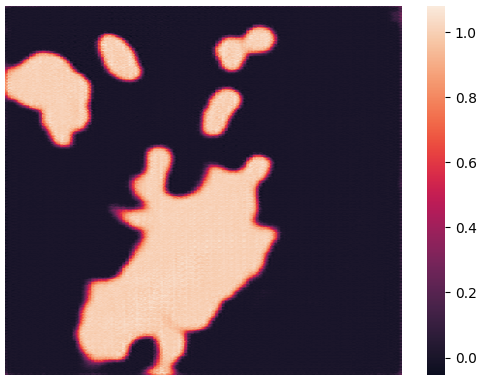
\includegraphics[width=0.3\columnwidth,   height=0.25\columnwidth]{imgs/hm_corrosion_erf.png} \\
        \footnotesize Image & \footnotesize CFM & \footnotesize DeepLab(Res101) & \footnotesize DeepLab(Xception) & \footnotesize DeepLab(MobileNet) & \footnotesize U-Net & \footnotesize ERFNet \\
    \end{tabular}
    \caption{The heat map of matting results: the first row shows the example from the BIO task, and the second row represents the example form COR task; the first column shows the input image, the matting results from CFM algorithm is shown in the second column; from the 3- to 7-th rows, the matting results from Res101-, Xception-, MobileNet-based DeepLabV3+ network, U-Net, and ERFNet are shown. }
    \label{fg:compare_matting_figure}
\end{figure*}

\begin{figure}[t]
    \centering
    \begin{tabular}{@{\hspace{0mm}}c@{\hspace{0.5mm}}c@{\hspace{0.5mm}}c@{\hspace{0.5mm}}c@{\hspace{0.5mm}}c@{\hspace{0mm}}}
        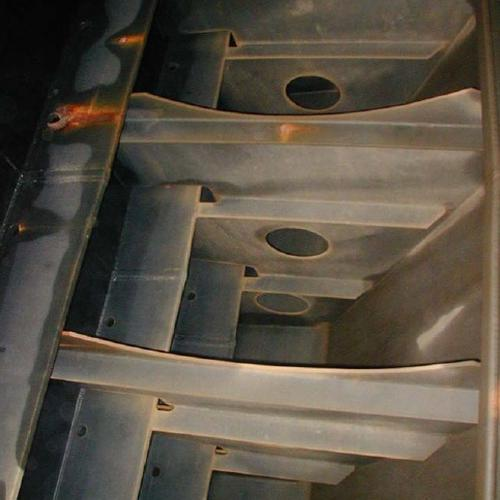
\includegraphics[width=0.25\columnwidth,   height=0.25\columnwidth]{imgs/image027_90.jpg} & 
        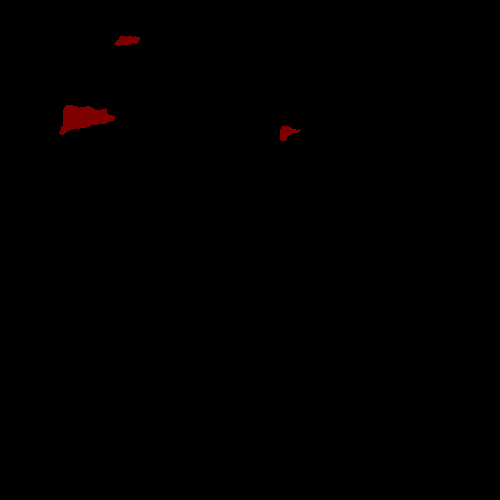
\includegraphics[width=0.25\columnwidth,   height=0.25\columnwidth]{imgs/image027_90_gt.png} &
        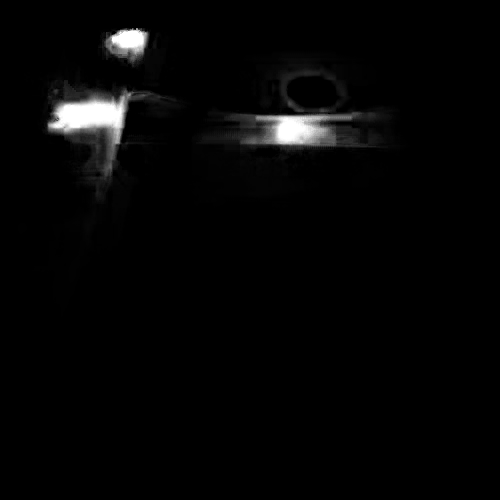
\includegraphics[width=0.25\columnwidth,   height=0.25\columnwidth]{imgs/image027_90_cfm.png} &
        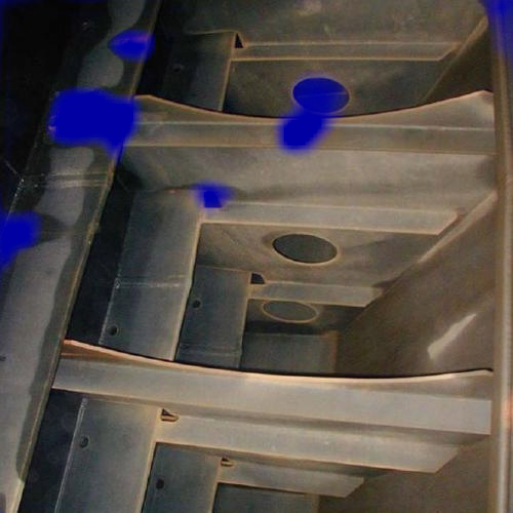
\includegraphics[width=0.25\columnwidth,   height=0.25\columnwidth]{imgs/image027_90_vis.png} \\
        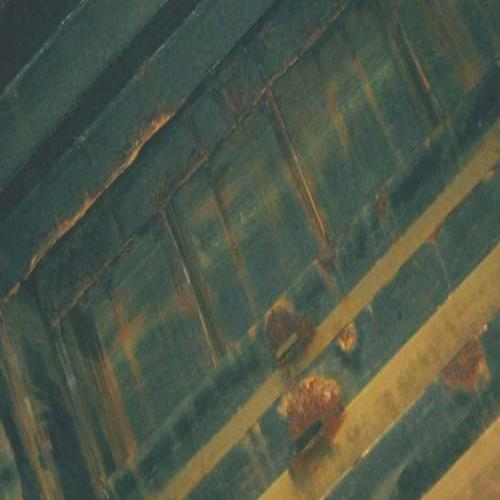
\includegraphics[width=0.25\columnwidth,   height=0.25\columnwidth]{imgs/image034_30.jpg} & 
        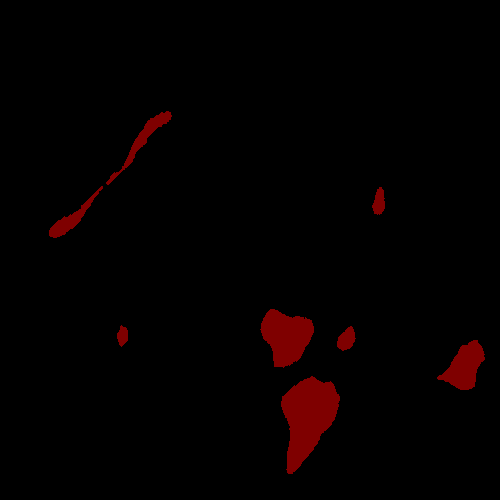
\includegraphics[width=0.25\columnwidth,   height=0.25\columnwidth]{imgs/image034_30_gt.png} &
        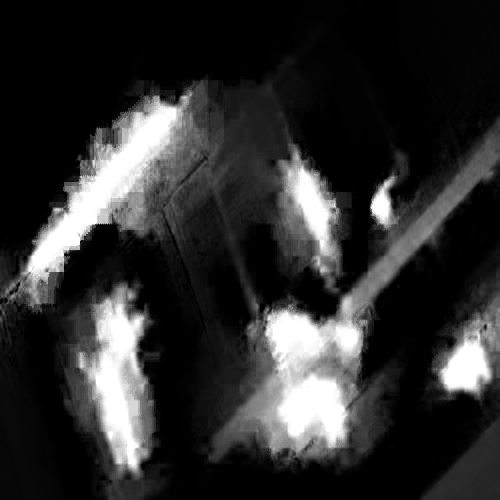
\includegraphics[width=0.25\columnwidth,   height=0.25\columnwidth]{imgs/image034_30_cfm.png} &
        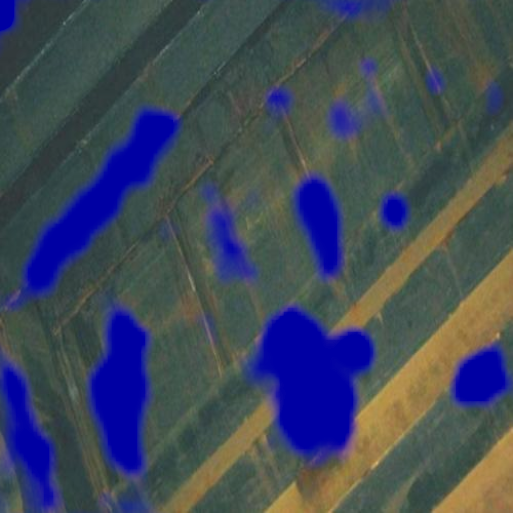
\includegraphics[width=0.25\columnwidth,   height=0.25\columnwidth]{imgs/image034_30_vis.png}  \\
        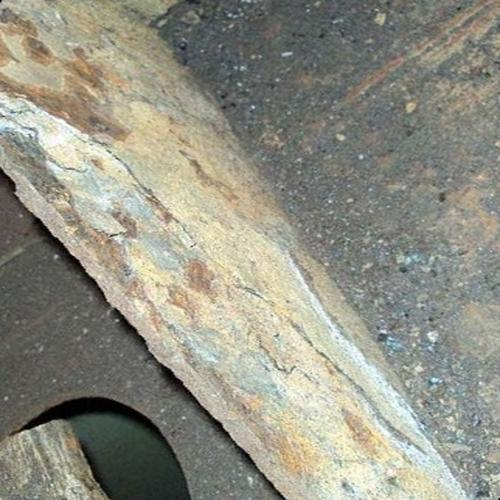
\includegraphics[width=0.25\columnwidth,   height=0.25\columnwidth]{imgs/image065_60.jpg} & 
        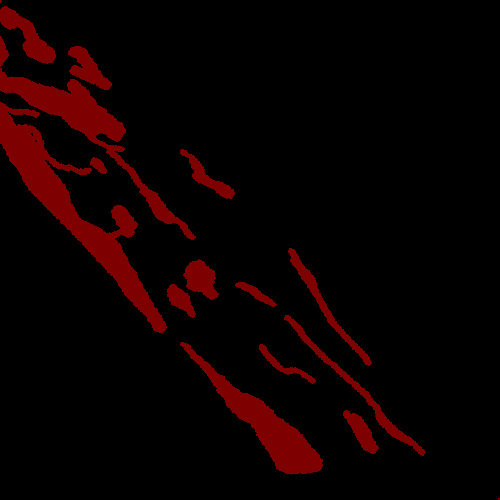
\includegraphics[width=0.25\columnwidth,   height=0.25\columnwidth]{imgs/image065_60_gt.png} &
        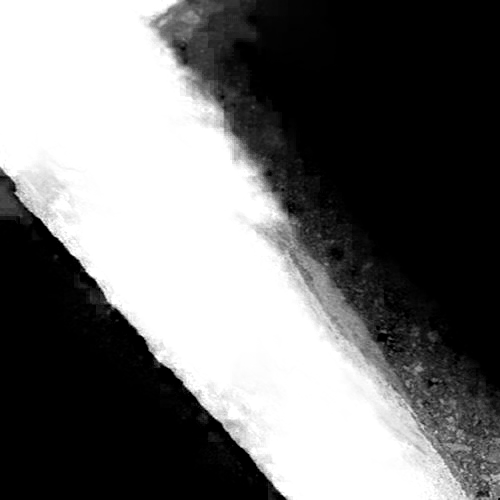
\includegraphics[width=0.25\columnwidth,   height=0.25\columnwidth]{imgs/image065_60_cfm.png} &
        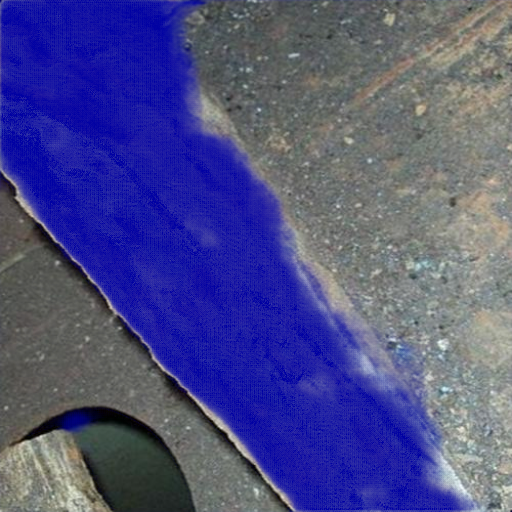
\includegraphics[width=0.25\columnwidth,   height=0.25\columnwidth]{imgs/image065_60_vis.png}  \\
        \footnotesize Image & \footnotesize GT & \footnotesize CFM & \footnotesize Ours
    \end{tabular}
    \caption{Examples of matting results and ground truth of the COR task.}
    \label{fg:comp_cor_matte_results}
\end{figure}

In Table \ref{tab:compare_matting_table}, we compute the MSE, mAD, and GE to evaluate how close the solution of our approach is to the solution of the CFM algorithm. Particularly, applying different backbones in the DeepLabV3+ module for our two tasks, the values of MSE, mAD, and GE is slightly different on both training and validation set. The performance of U-Net for the BIO task is slightly lower than the performance of the DeepLabV3+ network, while its performance for the COR task is close to DeepLabV3+. Notice that, for the small-scale network, such as the ERFNet (6.87MB parameters) and DeepLabV3+ (MobileNet as the backbone, 23.6 MB parameters), our approach also can achieve substantial performance as shown in Table \ref{tab:compare_matting_table}.

On the other hand, observing the values of metrics in Table \ref{tab:compare_matting_table}, different segmentation networks, that are trained by our loss function, obtain similar matting performance for our two inspection tasks. Therefore, the CFM loss can be used in different segmentation backbones.

\begin{table*}[t]
    \centering
    \caption{Metrics for the different experiments performed, varying the segmentation network. MSE stands for the mean square error, mAD indicates the mean sum of absolute difference, and GE represents the Gradient Error.}
    \label{tab:compare_matting_table}
    \begin{tabular}{p{1.5cm}p{5cm}p{2cm}p{2cm}p{2cm}}
        \toprule
        \textbf{Dataset} & \textbf{Network (backbone)}         & \textbf{MSE} & \textbf{mAD} & \textbf{GE} \\
        \midrule %\midrule
        \multirow{5}{1.5cm}{BioFouling (training set)}
        & DeepLabV3+ (ResNet-101)             & 0.0286       & 0.0822       & 2.1313                  \\
        & DeepLabV3+ (Xception)               & 0.0266       & 0.0751       & 2.2626                  \\
        & DeepLabV3+ (MobileNet)              & 0.0296       & 0.0811       & 2.0556                  \\
        & U-Net                               & 0.0599       & 0.1404       & 2.9092                  \\
        & ERFNet                              & 0.0480       & 0.1128       & 2.1250                  \\
        \midrule
        \multirow{5}{1.5cm}{BioFouling (validation set)}
        & DeepLabV3+ (ResNet-101)             & 0.0302       & 0.0837       & 1.7876                  \\
        & DeepLabV3+ (Xception)               & 0.0309       & 0.0821       & 1.9361                  \\
        & DeepLabV3+ (MobileNet)              & 0.0349       & 0.0889       & 1.6987                  \\
        & U-Net                               & 0.0625       & 0.1446       & 2.7250                  \\
        & ERFNet                              & 0.0501       & 0.1151       & 1.8171                  \\
        \midrule 
        \multirow{5}{1.5cm}{Corrosion (training set)}
        & DeepLabV3+ (ResNet-101)             & 0.0368       & 0.0829       & 1.9733                  \\
        & DeepLabV3+ (Xception)               & 0.0443       & 0.1017       & 2.1341                  \\
        & DeepLabV3+ (MobileNet)              & 0.0341       & 0.0793       & 1.9124                  \\
        & U-Net                               & 0.0467       & 0.0993       & 2.3060                  \\
        & ERFNet                              & 0.0407       & 0.0871       & 2.2085                  \\
        \midrule 
        \multirow{5}{1.5cm}{Corrosion (validation set)}
        & DeepLabV3+ (ResNet-101)             & 0.0399       & 0.0893       & 1.9401                  \\
        & DeepLabV3+ (Xception)               & 0.0519       & 0.1146       & 2.1266                  \\
        & DeepLabV3+ (MobileNet)              & 0.0363       & 0.0845       & 1.8927                  \\
        & U-Net                               & 0.0457       & 0.0981       & 2.4294                  \\
        & ERFNet                              & 0.0432       & 0.0925       & 2.1210                  \\
        \bottomrule
    \end{tabular}
\end{table*}

\subsection{Segmentation Results of Inspection Tasks}
\label{sec:seg_performance_ins}
\begin{table*}[t]
    \centering
    \caption{List of segmentation metrics on the validation set for the two inspection tasks. \textit{Network(backbone)} refers the segmentation network involved in our solution; \textit{\#TH} stands for the threshold to get the segmentation result based on the matting results; \textit{mIOU} represents the mean intersection over union; \textit{Rec}, \textit{Prec}, and \textit{F1} indicates the recall, precision, and F1 respectively. Best performance is highlighted in bold. }
    \label{tab:compare_seg_table}
    \begin{tabular}{p{1.5cm}p{3.5cm}p{1cm}p{1cm}p{1cm}p{1cm}p{1cm}}
        \toprule
        \textbf{Dataset} & \textbf{Network (backbone)}  & \textbf{\#TH}  & \textbf{mIOU} & \textbf{Rec} & \textbf{Prec} & \textbf{F1} \\
        \midrule %\midrule
        \multirow{20}{1.5cm}{BioFouling} 
        & \multirow{4}{3.5cm}{DeepLabV3+ (ResNet-101)}  & 0.4      & 0.8264           & \textbf{0.9285} & 0.8115          & 0.8660             \\
        &                                               & 0.5      & 0.8345           & 0.9139          & 0.8338          & 0.8720             \\
        &                                               & 0.6      & 0.8393           & 0.8972          & 0.8545          & 0.8753             \\
        &                                               & 0.7      & \textbf{0.8403}  & 0.8754          & \textbf{0.8759} & \textbf{0.8756}    \\
        \cmidrule{2-7}
        & \multirow{4}{3.5cm}{DeepLabV3+ (Xception)}    & 0.4      & 0.8262           & \textbf{0.9164} & 0.8158          & 0.8685             \\
        &                                               & 0.5      & 0.8338           & 0.8973          & 0.8414          & 0.8761             \\
        &                                               & 0.6      & \textbf{0.8367}  & 0.8760          & 0.8643          & 0.8804             \\
        &                                               & 0.7      & 0.8342           & 0.8488          & \textbf{0.8866} & \textbf{0.8809}    \\
        \cmidrule{2-7}
        & \multirow{4}{3.5cm}{DeepLabV3+ (Mobilenet)}   & 0.4      & 0.8193           & \textbf{0.9453} & 0.7851          & 0.8577             \\
        &                                               & 0.5      & 0.8284           & 0.9319          & 0.8072          & 0.8650             \\
        &                                               & 0.6      & 0.8340           & 0.9162          & 0.8281          & 0.8699             \\
        &                                               & 0.7      & \textbf{0.8359}  & 0.8957          & \textbf{0.8498} & \textbf{0.8721}    \\
        \cmidrule{2-7}
        & \multirow{4}{3.5cm}{U-Net}                    & 0.4      & 0.7134           & \textbf{0.8273} & 0.7101          & 0.7642             \\
        &                                               & 0.5      & \textbf{0.7191}  & 0.7871          & 0.7436          & \textbf{0.7647}    \\
        &                                               & 0.6      & 0.7161           & 0.7420          & 0.7737          & 0.7575             \\
        &                                               & 0.7      & 0.7024           & 0.6836          & \textbf{0.8043} & 0.7390             \\
        \cmidrule{2-7}
        & \multirow{4}{3.5cm}{ERFNet}                   & 0.4      & 0.7477           & \textbf{0.8142} & 0.7712          & \textbf{0.7921}    \\
        &                                               & 0.5      & \textbf{0.7488}  & 0.7801          & 0.8007          & 0.7902             \\
        &                                               & 0.6      & 0.7440           & 0.7436          & 0.8275          & 0.7833             \\
        &                                               & 0.7      & 0.7308           & 0.6972          & \textbf{0.8560} & 0.7684             \\
        \midrule
        \multirow{20}{1.5cm}{Corrosion} 
        & \multirow{4}{3.5cm}{DeepLabV3+ (ResNet-101)}  & 0.4      & 0.6758           & \textbf{0.9559} & 0.4777          & 0.6370             \\
        &                                               & 0.5      & 0.6879           & 0.9499          & 0.4970          & 0.6525             \\
        &                                               & 0.6      & 0.6986           & 0.9432          & 0.5155          & 0.6666             \\
        &                                               & 0.7      & \textbf{0.7093}  & 0.9350          & \textbf{0.5352} & \textbf{0.6807}    \\
        \cmidrule{2-7}
        & \multirow{4}{3.5cm}{DeepLabV3+ (Xception)}    & 0.4      & 0.6658           & \textbf{0.9374} & 0.4715          & 0.6274             \\
        &                                               & 0.5      & 0.6872           & 0.9199          & 0.5057          & 0.6526             \\
        &                                               & 0.6      & 0.7049           & 0.8983          & 0.5391          & 0.6738             \\
        &                                               & 0.7      & \textbf{0.7194}  & 0.8678          & \textbf{0.5744} & \textbf{0.6912}    \\
        \cmidrule{2-7}
        & \multirow{4}{3.5cm}{DeepLabV3+ (Mobilenet)}   & 0.4      & 0.6742           & \textbf{0.9566} & 0.4754          & 0.6351             \\
        &                                               & 0.5      & 0.6850           & 0.9526          & 0.4922          & 0.6490             \\
        &                                               & 0.6      & 0.6951           & 0.9479          & 0.5087          & 0.6620             \\
        &                                               & 0.7      & \textbf{0.7059}  & 0.9418          & \textbf{0.5273} & \textbf{0.6760}    \\
        \cmidrule{2-7}
        & \multirow{4}{3.5cm}{U-Net}                    & 0.4      & 0.7038           & \textbf{0.8825} & 0.5610          & 0.6859             \\
        &                                               & 0.5      & 0.7083           & 0.8662          & 0.5772          & 0.6927             \\
        &                                               & 0.6      & 0.7111           & 0.8478          & 0.5930          & 0.6978             \\
        &                                               & 0.7      & \textbf{0.7122}  & 0.8226          & \textbf{0.6113} & \textbf{0.7013}    \\
        \cmidrule{2-7}
        & \multirow{4}{3.5cm}{ERFNet}                   & 0.4      & 0.6742           & \textbf{0.9303} & 0.4847          & 0.6373             \\
        &                                               & 0.5      & 0.6826           & 0.9241          & 0.4984          & 0.6475             \\
        &                                               & 0.6      & 0.6886           & 0.9175          & 0.5123          & 0.6574             \\
        &                                               & 0.7      & \textbf{0.6973}  & 0.9088          & \textbf{0.5284} & \textbf{0.6682}    \\
        \bottomrule
    \end{tabular}
\end{table*}
To evaluate the segmentation performance of our approach, we measure the metrics on the two inspection tasks. For the BIO task, it is expensive in cost and time to obtain the pixel-level ground truth. Therefore, we obtain its ground truth by thresholding the CFM results, where the threshold is set to 0.5. Regarding the COR task, the pixel-level ground truth is used to evaluate the segmentation performance. Table \ref{tab:compare_seg_table} displays the metrics of segmentation performance. In order to obtain the segmentation results, four thresholds (from 0.4 to 0.7) are set for the matting results. 

As for the COR task, compared to the mIOU and F1 score, our approach achieves the best performance when the threshold is set to 0.7. When the threshold is 0.4, the best recall is obtained. Since our approach propagates scribble annotations to the entire image by minimizing the quadratic cost function, it can provide the suspicious regions according to how similar to the features of scribble annotations. On the other hand, these suspicious regions are not labelled due to their small scale and low hazard, but it is useful for us to analyze the inspection results. As shown in Fig. \ref{fg:comp_cor_matte_results}, the matte results provide useful suspicious corrosion regions, that are not labelled in the ground truth. Therefore, it can explain the reason that precision values for the COR task are low. Conversely, our approach achieves high recall values. In all, our approach can provide reliable COR results. 

As for the BIO task, three DeepLabV3+ models obtain outstanding segmentation performance than U-Net and ERFNet. Compared to metrics of DeepLabV3+ models, it is clear that when the threshold is set to 0.7, DeepLabV3+ with ResNet101 and Xception attains the highest recall, mIOU, and the highest precision, F1 score, respectively. For the MobileNet-based network, which only has 23.6 MB parameters, it obtains 0.8359 mIOU and 0.8721 F1 scores. Thus, even using a small-scale segmentation network, our approach can provide reasonable inspection results.

\subsection{Segmentation Results of MCSS Tasks}
\label{sec:seg_performance_mcss}
We conduct experiments to evaluate the effectiveness of our approach for MCSS tasks, and all results are evaluated on the two subsets of Pascal VOC and CityScapes benchmarks. For comparison, the upper bound of our method corresponds to the configuration using full masks and the cross-entropy loss ($L_{\text{ce}}$) for training. The partial cross-entropy loss ($L_{\text{pce}}$) with scribble annotations is used as the lower bound of our approach. Besides, we try to use a combination loss of $L_{\text{pce}}$ and $L_{\text{cfm}}$ to compare the segmentation performance.

The experimental results are reported in Table \ref{tab:tab_ablation_voc} for the VOC subset, and in Table \ref{tab:tab_ablation_cityscape} for the CityScape subset. Different from the inspection task, the threshold (0.5) is used to obtain the segmentation results from the matting results of every category. 

In Table \ref{tab:tab_ablation_voc}, the comparison reflects that our approach has the outstanding performance than the $L_{\text{pce}}$ method, and the IOU of Dog class (0.7459) is higher than the IOU of fully-supervised approach (0.7250). For the network trained by the combinational loss function, it attains a lower segmentation performance than that of network trained by $L_{\text{cfm}}$. 
\begin{table*}[t]
    \centering
    \caption{Per-class IOU on validation set of PASCAL VOC 2012 subset.}
    \label{tab:tab_ablation_voc}
    \begin{tabular}{p{1.2cm}|p{1.5cm}|p{1.4cm}p{1cm}p{1cm}p{1cm}p{1cm}p{1cm}p{1cm}|p{1.5cm}}
        \toprule
        \textbf{Dataset} & \textbf{Method} & \textbf{Background} &\textbf{Plane} & \textbf{Bike} & \textbf{Person} & \textbf{Car} & \textbf{Dog} & \textbf{Cat} & \textbf{Average (mIOU)} \\
        \midrule %\midrule
        \multirow{3}{1.2cm}{VOC subset}
        & $L_{\text{pce}}$                      & 0.7127       & 0.2427       & 0.0616   & 0.2871   & 0.1296   & 0.1626   & 0.3080   & 0,3121            \\
        & $L_{\text{cfm}}$                      & 0.9084       & 0.6136       & 0.5901   & 0.6066   & 0.6420   & 0.7459   & 0.8082   & 0,7020            \\
        & $L_{\text{cfm}}+L_{\text{pce}}$       & 0.8651       & 0.5386       & 0.5296   & 0.6242   & 0.5884   & 0.6782   & 0.7395   & 0,6519            \\
        & $L_{\text{ce}}$                       & 0.9379       & 0.7162       & 0.6439   & 0.6883   & 0.6882   & 0.7250   & 0.8552   & 0,7506            \\
        \bottomrule
    \end{tabular}
\end{table*}

For the subset of CityScape, training with our loss function obtains higher mIOU than the network training through $L_{\text{pce}}$ loss, as shown in Table \ref{tab:tab_ablation_cityscape}. Compared to the fully-supervised approach, the mIOU is 0.7136, which is 0.0731 higher than our approach. However, for the relatively big target, such as Road, Building, Sidewalk, Plant, Sky, and Car, our approach has a similar performance to the fully-supervised approach. Same as the experiment on the VOC subset, $L_{\text{pce}}$ has a negative effect on the segmentation performance in the case of combinational loss function.

\begin{table*}[t]
    \centering
    \caption{Per-class IOU on the validation set of CityScape subset.}
    \label{tab:tab_ablation_cityscape}
    \begin{tabular}{p{1.5cm}|p{1.5cm}|p{0.8cm}p{0.8cm}p{0.8cm}p{0.8cm}p{0.8cm}p{0.8cm}p{0.8cm}p{0.8cm}p{0.8cm}|p{1.5cm}}
        \toprule
        \textbf{Dataset} & \textbf{Method} & \textbf{Road} &\textbf{Building} & \textbf{Sidewalk} & \textbf{Traffic Sign} & \textbf{Plant} & \textbf{Sky} & \textbf{Person} & \textbf{Car} & \textbf{Bike} & \textbf{Average (mIOU)} \\
        \midrule %\midrule
        \multirow{3}{1.5cm}{CityScape subset}
        & $L_{\text{pce}}                 $     & 0.7025       & 0.3666       & 0.5617   & 0.1207   & 0.6120   & 0.5599   & 0.1773   & 0.5513   & 0.2573   & 0.4343         \\
        & $L_{\text{cfm}}                 $     & 0.7561       & 0.5942       & 0.7083   & 0.4731   & 0.7623   & 0.7727   & 0.5723   & 0.6760   & 0.4503   & 0.6405         \\
        & $L_{\text{cfm}}+L_{\text{pce}}  $     & 0.6763       & 0.5494       & 0.6816   & 0.4928   & 0.6418   & 0.6838   & 0.5774   & 0.5988   & 0.4024   & 0.5893         \\
        & $L_{\text{ce}}                  $     & 0.9084       & 0.7136       & 0.7301   & 0.6066   & 0.7420   & 0.7850   & 0.7082   & 0,6991   & 0.5296   & 0.7136         \\
        \bottomrule
    \end{tabular}
\end{table*}




\subsection{Experimental Results Visualization}
\label{sec:vis_exp_results}
In Fig. \ref{fg:vis_bio_results} and \ref{fg:vis_corrosion_results}, some samples from BioFouling and COR tasks are shown, respectively. For one input image, the first row displays the input image firstly, then the scribble annotation is shown, and the rest in the first row displays the segmentation network. For both tasks, the segmentation results are obtained by setting the threshold to 0.7. The second row firstly shows the evaluation ground truth; secondly, the matting results of the CFM algorithm are shown. The rest of the image in the second row are the matting results from our solution.

As shown in Fig. \ref{fg:vis_bio_results} and \ref{fg:vis_corrosion_results}, our approach can obtain similar matting results to the CFM algorithm, which provides considerable segmentation results by thresholding. 
% Moreover, after training, our approach does not need to use scribble annotations during inference and needs less running time than the CFM algorithm.

For the MCSS problems, the segmentation results on the subsets of VOC and CityScape, which are obtained by thresholding on the matting results, are shown in Fig. \ref{fg:vis_voc_results} and \ref{fg:vis_cityscape_results}, respectively. As can be observed, our approach achieves a considerable matting performance for every category. At the end, we set the threshold of 0.5 to the matting results on each category to get the final segmentation results. As can be seen in Fig. \ref{fg:vis_voc_results} and \ref{fg:vis_cityscape_results}, our approach gets a good segmentation performance for different MCSS tasks.

In conclusion, the network, trained by our CFM loss function with scribble annotations, can obtain a reliable segmentation performance for the Inspection and MCSS tasks.

\begin{figure*}[t]
    \centering
    \begin{tabular}{@{\hspace{0mm}}c@{\hspace{0.5mm}}c@{\hspace{0.5mm}}c@{\hspace{0.5mm}}c@{\hspace{0.5mm}}c@{\hspace{0.5mm}}c@{\hspace{0.5mm}}c@{\hspace{0mm}}}
        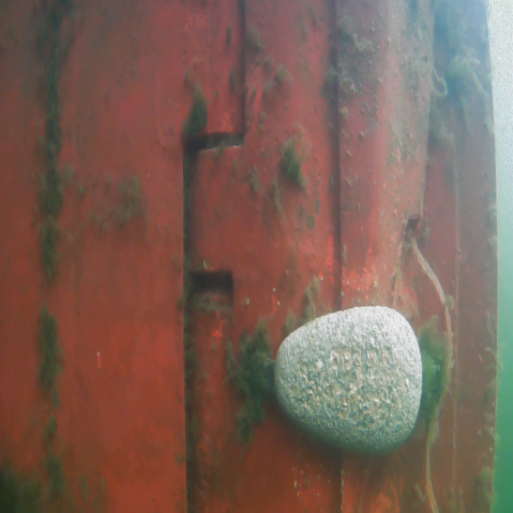
\includegraphics[width=0.25\columnwidth,   height=0.25\columnwidth]{imgs/results/biofouling/org/beye_01_001000.png} &
        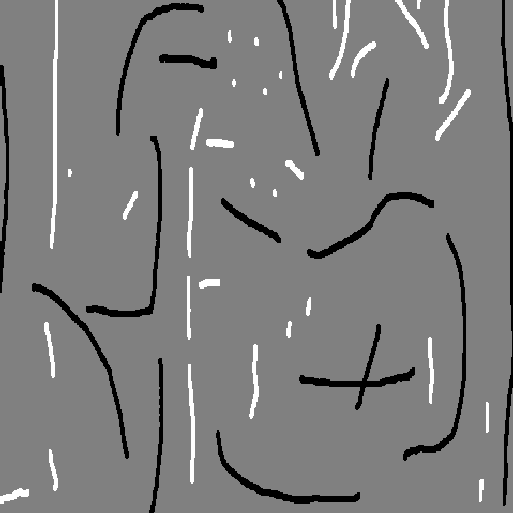
\includegraphics[width=0.25\columnwidth,   height=0.25\columnwidth]{imgs/results/biofouling/gt/beye_01_001000.png} &
        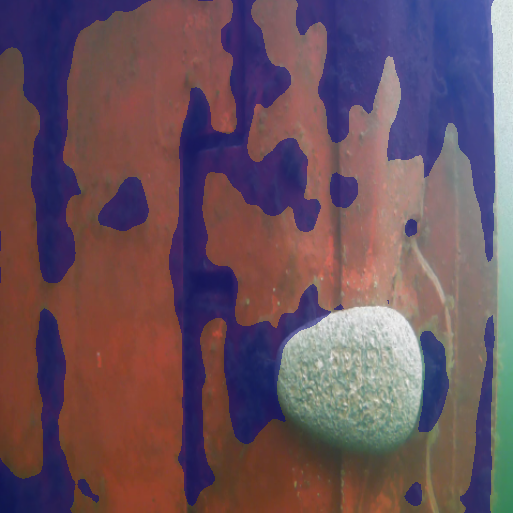
\includegraphics[width=0.25\columnwidth,   height=0.25\columnwidth]{imgs/results/biofouling/res101/beye_01_001000.png} &
        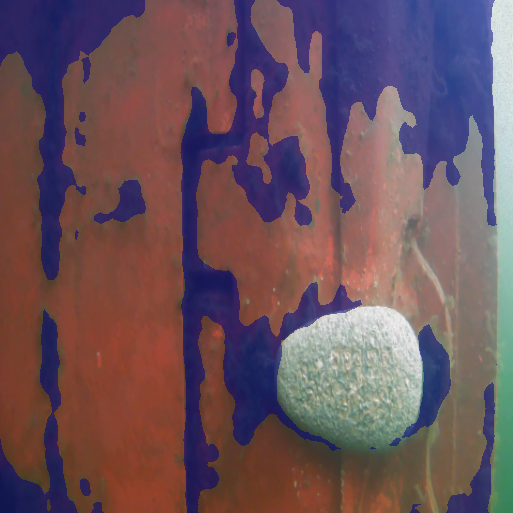
\includegraphics[width=0.25\columnwidth,   height=0.25\columnwidth]{imgs/results/biofouling/xception/beye_01_001000.png} &
        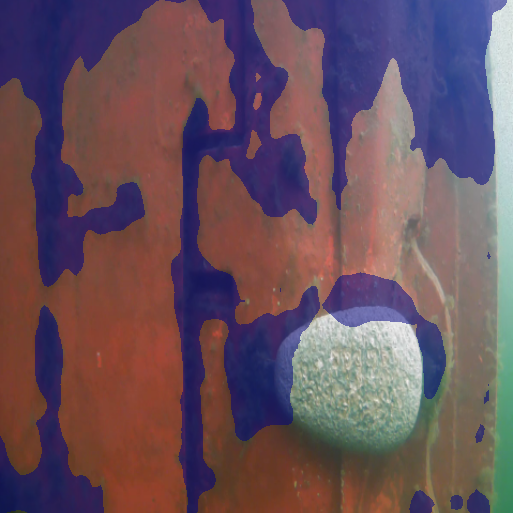
\includegraphics[width=0.25\columnwidth,   height=0.25\columnwidth]{imgs/results/biofouling/mobilenet/beye_01_001000.png} &
        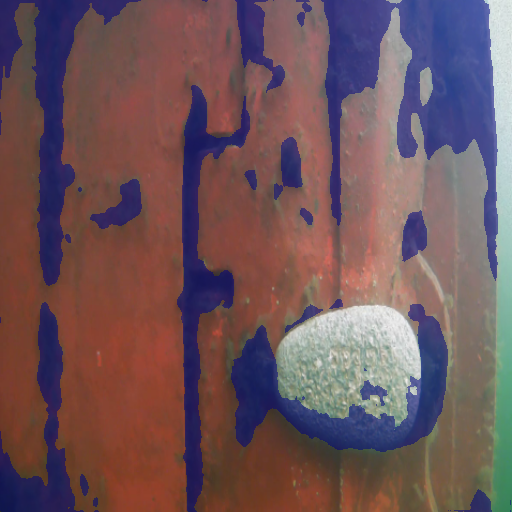
\includegraphics[width=0.25\columnwidth,   height=0.25\columnwidth]{imgs/results/biofouling/unet/beye_01_001000.png} &
        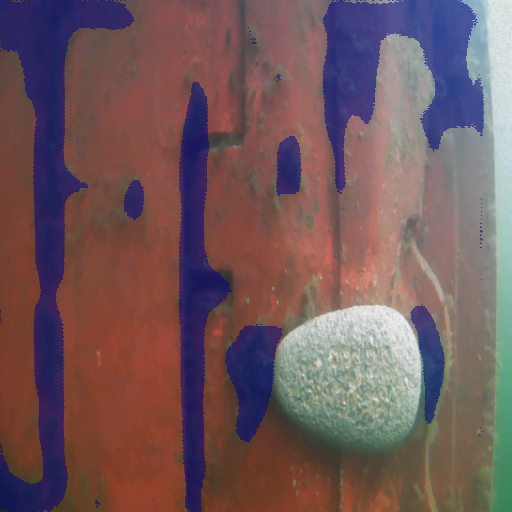
\includegraphics[width=0.25\columnwidth,   height=0.25\columnwidth]{imgs/results/biofouling/erf/beye_01_001000.png} \\ 

        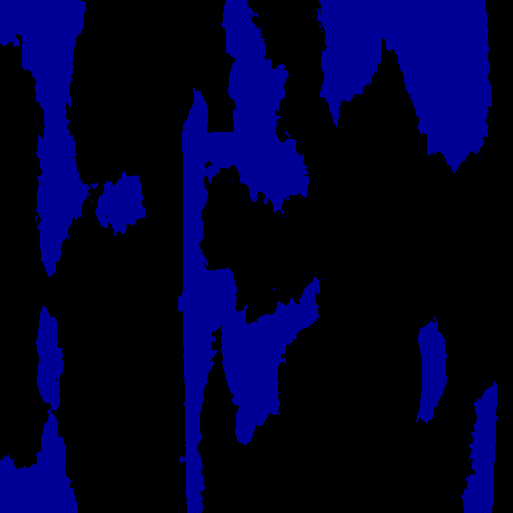
\includegraphics[width=0.25\columnwidth,   height=0.25\columnwidth]{imgs/results/biofouling/gt/beye_01_001000_gt.png} &
        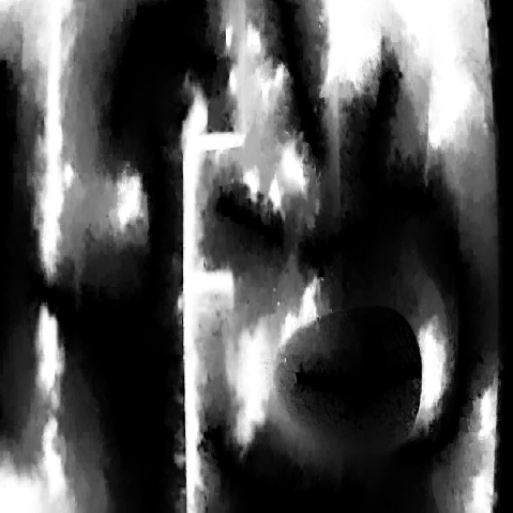
\includegraphics[width=0.25\columnwidth,   height=0.25\columnwidth]{imgs/results/biofouling/cfm/beye_01_001000.png} &
        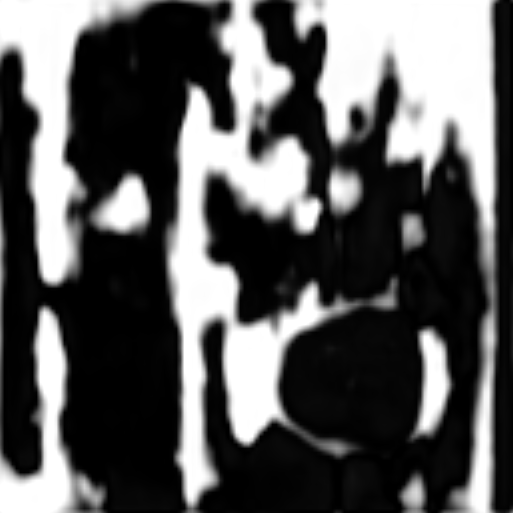
\includegraphics[width=0.25\columnwidth,   height=0.25\columnwidth]{imgs/results/biofouling/res101/beye_01_001000_alpha.png} &
        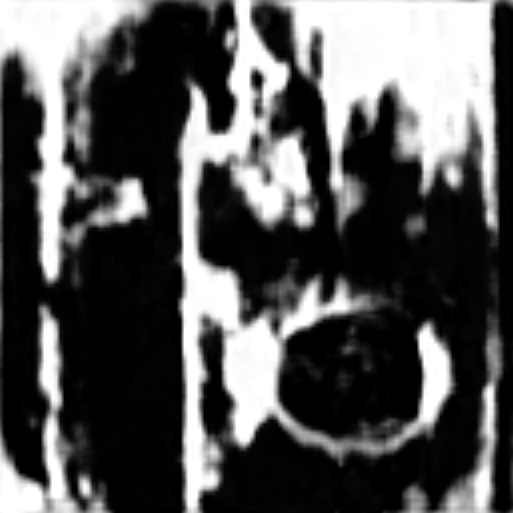
\includegraphics[width=0.25\columnwidth,   height=0.25\columnwidth]{imgs/results/biofouling/xception/beye_01_001000_alpha.png} &
        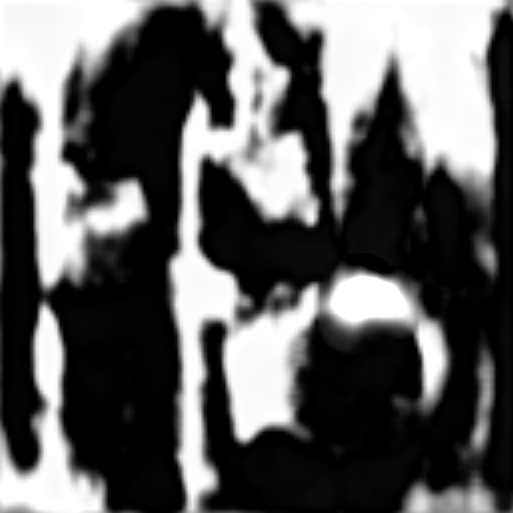
\includegraphics[width=0.25\columnwidth,   height=0.25\columnwidth]{imgs/results/biofouling/mobilenet/beye_01_001000_alpha.png} &
        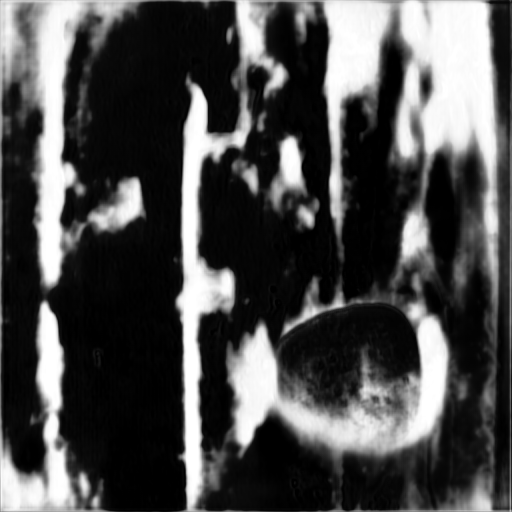
\includegraphics[width=0.25\columnwidth,   height=0.25\columnwidth]{imgs/results/biofouling/unet/beye_01_001000_alpha.png} &
        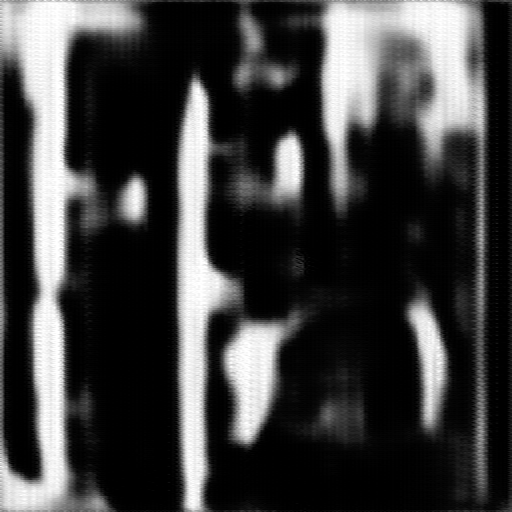
\includegraphics[width=0.25\columnwidth,   height=0.25\columnwidth]{imgs/results/biofouling/erf/beye_01_001000_alpha.png} \\

        \includegraphics[width=0.25\columnwidth,   height=0.25\columnwidth]{imgs/results/biofouling/org/beye_13_009900.png} &
        \includegraphics[width=0.25\columnwidth,   height=0.25\columnwidth]{imgs/results/biofouling/gt/beye_13_009900.png} &
        \includegraphics[width=0.25\columnwidth,   height=0.25\columnwidth]{imgs/results/biofouling/res101/beye_13_009900.png} &
        \includegraphics[width=0.25\columnwidth,   height=0.25\columnwidth]{imgs/results/biofouling/xception/beye_13_009900.png} &
        \includegraphics[width=0.25\columnwidth,   height=0.25\columnwidth]{imgs/results/biofouling/mobilenet/beye_13_009900.png} &
        \includegraphics[width=0.25\columnwidth,   height=0.25\columnwidth]{imgs/results/biofouling/unet/beye_13_009900.png} &
        \includegraphics[width=0.25\columnwidth,   height=0.25\columnwidth]{imgs/results/biofouling/erf/beye_13_009900.png} \\ 

        \includegraphics[width=0.25\columnwidth,   height=0.25\columnwidth]{imgs/results/biofouling/gt/beye_13_009900_gt.png} &
        \includegraphics[width=0.25\columnwidth,   height=0.25\columnwidth]{imgs/results/biofouling/cfm/beye_13_009900.png} &
        \includegraphics[width=0.25\columnwidth,   height=0.25\columnwidth]{imgs/results/biofouling/res101/beye_13_009900_alpha.png} &
        \includegraphics[width=0.25\columnwidth,   height=0.25\columnwidth]{imgs/results/biofouling/xception/beye_13_009900_alpha.png} &
        \includegraphics[width=0.25\columnwidth,   height=0.25\columnwidth]{imgs/results/biofouling/mobilenet/beye_13_009900_alpha.png} &
        \includegraphics[width=0.25\columnwidth,   height=0.25\columnwidth]{imgs/results/biofouling/unet/beye_13_009900_alpha.png} &
        \includegraphics[width=0.25\columnwidth,   height=0.25\columnwidth]{imgs/results/biofouling/erf/beye_13_009900_alpha.png} \\  

        \includegraphics[width=0.25\columnwidth,   height=0.25\columnwidth]{imgs/results/biofouling/org/beye_16_000300.png} &
        \includegraphics[width=0.25\columnwidth,   height=0.25\columnwidth]{imgs/results/biofouling/gt/beye_16_000300.png} &
        \includegraphics[width=0.25\columnwidth,   height=0.25\columnwidth]{imgs/results/biofouling/res101/beye_16_000300.png} &
        \includegraphics[width=0.25\columnwidth,   height=0.25\columnwidth]{imgs/results/biofouling/xception/beye_16_000300.png} &
        \includegraphics[width=0.25\columnwidth,   height=0.25\columnwidth]{imgs/results/biofouling/mobilenet/beye_16_000300.png} &
        \includegraphics[width=0.25\columnwidth,   height=0.25\columnwidth]{imgs/results/biofouling/unet/beye_16_000300.png} &
        \includegraphics[width=0.25\columnwidth,   height=0.25\columnwidth]{imgs/results/biofouling/erf/beye_16_000300.png} \\ 

        \includegraphics[width=0.25\columnwidth,   height=0.25\columnwidth]{imgs/results/biofouling/gt/beye_16_000300_gt.png} &
        \includegraphics[width=0.25\columnwidth,   height=0.25\columnwidth]{imgs/results/biofouling/cfm/beye_16_000300.png} &
        \includegraphics[width=0.25\columnwidth,   height=0.25\columnwidth]{imgs/results/biofouling/res101/beye_16_000300_alpha.png} &
        \includegraphics[width=0.25\columnwidth,   height=0.25\columnwidth]{imgs/results/biofouling/xception/beye_16_000300_alpha.png} &
        \includegraphics[width=0.25\columnwidth,   height=0.25\columnwidth]{imgs/results/biofouling/mobilenet/beye_16_000300_alpha.png} &
        \includegraphics[width=0.25\columnwidth,   height=0.25\columnwidth]{imgs/results/biofouling/unet/beye_16_000300_alpha.png} &
        \includegraphics[width=0.25\columnwidth,   height=0.25\columnwidth]{imgs/results/biofouling/erf/beye_16_000300_alpha.png} \\ 

        \includegraphics[width=0.25\columnwidth,   height=0.25\columnwidth]{imgs/results/biofouling/org/beye_16_003500.png} &
        \includegraphics[width=0.25\columnwidth,   height=0.25\columnwidth]{imgs/results/biofouling/gt/beye_16_003500.png} &
        \includegraphics[width=0.25\columnwidth,   height=0.25\columnwidth]{imgs/results/biofouling/res101/beye_16_003500.png} &
        \includegraphics[width=0.25\columnwidth,   height=0.25\columnwidth]{imgs/results/biofouling/xception/beye_16_003500.png} &
        \includegraphics[width=0.25\columnwidth,   height=0.25\columnwidth]{imgs/results/biofouling/mobilenet/beye_16_003500.png} &
        \includegraphics[width=0.25\columnwidth,   height=0.25\columnwidth]{imgs/results/biofouling/unet/beye_16_003500.png} &
        \includegraphics[width=0.25\columnwidth,   height=0.25\columnwidth]{imgs/results/biofouling/erf/beye_16_003500.png} \\ 

        \includegraphics[width=0.25\columnwidth,   height=0.25\columnwidth]{imgs/results/biofouling/gt/beye_16_003500_gt.png} &
        \includegraphics[width=0.25\columnwidth,   height=0.25\columnwidth]{imgs/results/biofouling/cfm/beye_16_003500.png} &
        \includegraphics[width=0.25\columnwidth,   height=0.25\columnwidth]{imgs/results/biofouling/res101/beye_16_003500_alpha.png} &
        \includegraphics[width=0.25\columnwidth,   height=0.25\columnwidth]{imgs/results/biofouling/xception/beye_16_003500_alpha.png} &
        \includegraphics[width=0.25\columnwidth,   height=0.25\columnwidth]{imgs/results/biofouling/mobilenet/beye_16_003500_alpha.png} &
        \includegraphics[width=0.25\columnwidth,   height=0.25\columnwidth]{imgs/results/biofouling/unet/beye_16_003500_alpha.png} &
        \includegraphics[width=0.25\columnwidth,   height=0.25\columnwidth]{imgs/results/biofouling/erf/beye_16_003500_alpha.png} \\ 

        \includegraphics[width=0.25\columnwidth,   height=0.25\columnwidth]{imgs/results/biofouling/org/beye_16_005400.png} &
        \includegraphics[width=0.25\columnwidth,   height=0.25\columnwidth]{imgs/results/biofouling/gt/beye_16_005400.png} &
        \includegraphics[width=0.25\columnwidth,   height=0.25\columnwidth]{imgs/results/biofouling/res101/beye_16_005400.png} &
        \includegraphics[width=0.25\columnwidth,   height=0.25\columnwidth]{imgs/results/biofouling/xception/beye_16_005400.png} &
        \includegraphics[width=0.25\columnwidth,   height=0.25\columnwidth]{imgs/results/biofouling/mobilenet/beye_16_005400.png} &
        \includegraphics[width=0.25\columnwidth,   height=0.25\columnwidth]{imgs/results/biofouling/unet/beye_16_005400.png} &
        \includegraphics[width=0.25\columnwidth,   height=0.25\columnwidth]{imgs/results/biofouling/erf/beye_16_005400.png} \\ 

        \includegraphics[width=0.25\columnwidth,   height=0.25\columnwidth]{imgs/results/biofouling/gt/beye_16_005400_gt.png} &
        \includegraphics[width=0.25\columnwidth,   height=0.25\columnwidth]{imgs/results/biofouling/cfm/beye_16_005400.png} &
        \includegraphics[width=0.25\columnwidth,   height=0.25\columnwidth]{imgs/results/biofouling/res101/beye_16_005400_alpha.png} &
        \includegraphics[width=0.25\columnwidth,   height=0.25\columnwidth]{imgs/results/biofouling/xception/beye_16_005400_alpha.png} &
        \includegraphics[width=0.25\columnwidth,   height=0.25\columnwidth]{imgs/results/biofouling/mobilenet/beye_16_005400_alpha.png} &
        \includegraphics[width=0.25\columnwidth,   height=0.25\columnwidth]{imgs/results/biofouling/unet/beye_16_005400_alpha.png} &
        \includegraphics[width=0.25\columnwidth,   height=0.25\columnwidth]{imgs/results/biofouling/erf/beye_16_005400_alpha.png} \\ 

        \footnotesize Image/GT & \footnotesize CFM/GT & \footnotesize DeepLab(Res101) & \footnotesize DeepLab(Xception) & \footnotesize DeepLab(MobileNet) & \footnotesize U-Net & \footnotesize ERFNet \\
    \end{tabular}
    \caption{Examples of segmentation and matting results for the BIO task. For every sample, the first image in the 1st row is the input image; and the 2nd image is the scribble annotation; from the 3- to 7-th, the images are the segmentation results using different segmentation network; in the second row, the first two images are the segmentation ground truth and matting results of the CFM algorithm; the rest images in the second row are the matting results of our approach by using different networks.}
    \label{fg:vis_bio_results}
\end{figure*}

\begin{figure*}[t]
    \centering
    \begin{tabular}{@{\hspace{0mm}}c@{\hspace{0.5mm}}c@{\hspace{0.5mm}}c@{\hspace{0.5mm}}c@{\hspace{0.5mm}}c@{\hspace{0.5mm}}c@{\hspace{0.5mm}}c@{\hspace{0mm}}}
        \includegraphics[width=0.25\columnwidth,   height=0.25\columnwidth]{imgs/results/corrosion/org/gk2_fp_exp29_0570_90_ROI.png} &
        \includegraphics[width=0.25\columnwidth,   height=0.25\columnwidth]{imgs/results/corrosion/gt/gk2_fp_exp29_0570_90_ROI.png} &
        \includegraphics[width=0.25\columnwidth,   height=0.25\columnwidth]{imgs/results/corrosion/res101/gk2_fp_exp29_0570_90_ROI.png} &
        \includegraphics[width=0.25\columnwidth,   height=0.25\columnwidth]{imgs/results/corrosion/xception/gk2_fp_exp29_0570_90_ROI.png} &
        \includegraphics[width=0.25\columnwidth,   height=0.25\columnwidth]{imgs/results/corrosion/mobilenet/gk2_fp_exp29_0570_90_ROI.png} &
        \includegraphics[width=0.25\columnwidth,   height=0.25\columnwidth]{imgs/results/corrosion/unet/gk2_fp_exp29_0570_90_ROI.png} &
        \includegraphics[width=0.25\columnwidth,   height=0.25\columnwidth]{imgs/results/corrosion/erf/gk2_fp_exp29_0570_90_ROI.png} \\ 

        \includegraphics[width=0.25\columnwidth,   height=0.25\columnwidth]{imgs/results/corrosion/gt/gk2_fp_exp29_0570_90_ROI_gt.png} &
        \includegraphics[width=0.25\columnwidth,   height=0.25\columnwidth]{imgs/results/corrosion/cfm/gk2_fp_exp29_0570_90_ROI.png} &
        \includegraphics[width=0.25\columnwidth,   height=0.25\columnwidth]{imgs/results/corrosion/res101/gk2_fp_exp29_0570_90_ROI_alpha.png} &
        \includegraphics[width=0.25\columnwidth,   height=0.25\columnwidth]{imgs/results/corrosion/xception/gk2_fp_exp29_0570_90_ROI_alpha.png} &
        \includegraphics[width=0.25\columnwidth,   height=0.25\columnwidth]{imgs/results/corrosion/mobilenet/gk2_fp_exp29_0570_90_ROI_alpha.png} &
        \includegraphics[width=0.25\columnwidth,   height=0.25\columnwidth]{imgs/results/corrosion/unet/gk2_fp_exp29_0570_90_ROI_alpha.png} &
        \includegraphics[width=0.25\columnwidth,   height=0.25\columnwidth]{imgs/results/corrosion/erf/gk2_fp_exp29_0570_90_ROI_alpha.png} \\

        \includegraphics[width=0.25\columnwidth,   height=0.25\columnwidth]{imgs/results/corrosion/org/image036_90.png} &
        \includegraphics[width=0.25\columnwidth,   height=0.25\columnwidth]{imgs/results/corrosion/gt/image036_90.png} &
        \includegraphics[width=0.25\columnwidth,   height=0.25\columnwidth]{imgs/results/corrosion/res101/image036_90.png} &
        \includegraphics[width=0.25\columnwidth,   height=0.25\columnwidth]{imgs/results/corrosion/xception/image036_90.png} &
        \includegraphics[width=0.25\columnwidth,   height=0.25\columnwidth]{imgs/results/corrosion/mobilenet/image036_90.png} &
        \includegraphics[width=0.25\columnwidth,   height=0.25\columnwidth]{imgs/results/corrosion/unet/image036_90.png} &
        \includegraphics[width=0.25\columnwidth,   height=0.25\columnwidth]{imgs/results/corrosion/erf/image036_90.png} \\ 

        \includegraphics[width=0.25\columnwidth,   height=0.25\columnwidth]{imgs/results/corrosion/gt/image036_90_gt.png} &
        \includegraphics[width=0.25\columnwidth,   height=0.25\columnwidth]{imgs/results/corrosion/cfm/image036_90.png} &
        \includegraphics[width=0.25\columnwidth,   height=0.25\columnwidth]{imgs/results/corrosion/res101/image036_90_alpha.png} &
        \includegraphics[width=0.25\columnwidth,   height=0.25\columnwidth]{imgs/results/corrosion/xception/image036_90_alpha.png} &
        \includegraphics[width=0.25\columnwidth,   height=0.25\columnwidth]{imgs/results/corrosion/mobilenet/image036_90_alpha.png} &
        \includegraphics[width=0.25\columnwidth,   height=0.25\columnwidth]{imgs/results/corrosion/unet/image036_90_alpha.png} &
        \includegraphics[width=0.25\columnwidth,   height=0.25\columnwidth]{imgs/results/corrosion/erf/image036_90_alpha.png} \\

        \includegraphics[width=0.25\columnwidth,   height=0.25\columnwidth]{imgs/results/corrosion/org/gk2_ts_exp19_1280_30.png} &
        \includegraphics[width=0.25\columnwidth,   height=0.25\columnwidth]{imgs/results/corrosion/gt/gk2_ts_exp19_1280_30.png} &
        \includegraphics[width=0.25\columnwidth,   height=0.25\columnwidth]{imgs/results/corrosion/res101/gk2_ts_exp19_1280_30.png} &
        \includegraphics[width=0.25\columnwidth,   height=0.25\columnwidth]{imgs/results/corrosion/xception/gk2_ts_exp19_1280_30.png} &
        \includegraphics[width=0.25\columnwidth,   height=0.25\columnwidth]{imgs/results/corrosion/mobilenet/gk2_ts_exp19_1280_30.png} &
        \includegraphics[width=0.25\columnwidth,   height=0.25\columnwidth]{imgs/results/corrosion/unet/gk2_ts_exp19_1280_30.png} &
        \includegraphics[width=0.25\columnwidth,   height=0.25\columnwidth]{imgs/results/corrosion/erf/gk2_ts_exp19_1280_30.png} \\ 

        \includegraphics[width=0.25\columnwidth,   height=0.25\columnwidth]{imgs/results/corrosion/gt/gk2_ts_exp19_1280_30_gt.png} &
        \includegraphics[width=0.25\columnwidth,   height=0.25\columnwidth]{imgs/results/corrosion/cfm/gk2_ts_exp19_1280_30.png} &
        \includegraphics[width=0.25\columnwidth,   height=0.25\columnwidth]{imgs/results/corrosion/res101/gk2_ts_exp19_1280_30_alpha.png} &
        \includegraphics[width=0.25\columnwidth,   height=0.25\columnwidth]{imgs/results/corrosion/xception/gk2_ts_exp19_1280_30_alpha.png} &
        \includegraphics[width=0.25\columnwidth,   height=0.25\columnwidth]{imgs/results/corrosion/mobilenet/gk2_ts_exp19_1280_30_alpha.png} &
        \includegraphics[width=0.25\columnwidth,   height=0.25\columnwidth]{imgs/results/corrosion/unet/gk2_ts_exp19_1280_30_alpha.png} &
        \includegraphics[width=0.25\columnwidth,   height=0.25\columnwidth]{imgs/results/corrosion/erf/gk2_ts_exp19_1280_30_alpha.png} \\

        \includegraphics[width=0.25\columnwidth,   height=0.25\columnwidth]{imgs/results/corrosion/org/image072_60.png} &
        \includegraphics[width=0.25\columnwidth,   height=0.25\columnwidth]{imgs/results/corrosion/gt/image072_60.png} &
        \includegraphics[width=0.25\columnwidth,   height=0.25\columnwidth]{imgs/results/corrosion/res101/image072_60.png} &
        \includegraphics[width=0.25\columnwidth,   height=0.25\columnwidth]{imgs/results/corrosion/xception/image072_60.png} &
        \includegraphics[width=0.25\columnwidth,   height=0.25\columnwidth]{imgs/results/corrosion/mobilenet/image072_60.png} &
        \includegraphics[width=0.25\columnwidth,   height=0.25\columnwidth]{imgs/results/corrosion/unet/image072_60.png} &
        \includegraphics[width=0.25\columnwidth,   height=0.25\columnwidth]{imgs/results/corrosion/erf/image072_60.png} \\ 

        \includegraphics[width=0.25\columnwidth,   height=0.25\columnwidth]{imgs/results/corrosion/gt/image072_60_gt.png} &
        \includegraphics[width=0.25\columnwidth,   height=0.25\columnwidth]{imgs/results/corrosion/cfm/image072_60.png} &
        \includegraphics[width=0.25\columnwidth,   height=0.25\columnwidth]{imgs/results/corrosion/res101/image072_60_alpha.png} &
        \includegraphics[width=0.25\columnwidth,   height=0.25\columnwidth]{imgs/results/corrosion/xception/image072_60_alpha.png} &
        \includegraphics[width=0.25\columnwidth,   height=0.25\columnwidth]{imgs/results/corrosion/mobilenet/image072_60_alpha.png} &
        \includegraphics[width=0.25\columnwidth,   height=0.25\columnwidth]{imgs/results/corrosion/unet/image072_60_alpha.png} &
        \includegraphics[width=0.25\columnwidth,   height=0.25\columnwidth]{imgs/results/corrosion/erf/image072_60_alpha.png} \\

        \includegraphics[width=0.25\columnwidth,   height=0.25\columnwidth]{imgs/results/corrosion/org/image065_90.png} &
        \includegraphics[width=0.25\columnwidth,   height=0.25\columnwidth]{imgs/results/corrosion/gt/image065_90.png} &
        \includegraphics[width=0.25\columnwidth,   height=0.25\columnwidth]{imgs/results/corrosion/res101/image065_90.png} &
        \includegraphics[width=0.25\columnwidth,   height=0.25\columnwidth]{imgs/results/corrosion/xception/image065_90.png} &
        \includegraphics[width=0.25\columnwidth,   height=0.25\columnwidth]{imgs/results/corrosion/mobilenet/image065_90.png} &
        \includegraphics[width=0.25\columnwidth,   height=0.25\columnwidth]{imgs/results/corrosion/unet/image065_90.png} &
        \includegraphics[width=0.25\columnwidth,   height=0.25\columnwidth]{imgs/results/corrosion/erf/image065_90.png} \\ 

        \includegraphics[width=0.25\columnwidth,   height=0.25\columnwidth]{imgs/results/corrosion/gt/image065_90_gt.png} &
        \includegraphics[width=0.25\columnwidth,   height=0.25\columnwidth]{imgs/results/corrosion/cfm/image065_90.png} &
        \includegraphics[width=0.25\columnwidth,   height=0.25\columnwidth]{imgs/results/corrosion/res101/image065_90_alpha.png} &
        \includegraphics[width=0.25\columnwidth,   height=0.25\columnwidth]{imgs/results/corrosion/xception/image065_90_alpha.png} &
        \includegraphics[width=0.25\columnwidth,   height=0.25\columnwidth]{imgs/results/corrosion/mobilenet/image065_90_alpha.png} &
        \includegraphics[width=0.25\columnwidth,   height=0.25\columnwidth]{imgs/results/corrosion/unet/image065_90_alpha.png} &
        \includegraphics[width=0.25\columnwidth,   height=0.25\columnwidth]{imgs/results/corrosion/erf/image065_90_alpha.png} \\

        \footnotesize Image/GT & \footnotesize CFM/GT & \footnotesize DeepLab(Res101) & \footnotesize DeepLab(Xception) & \footnotesize DeepLab(MobileNet) & \footnotesize U-Net & \footnotesize ERFNet \\
    \end{tabular}
    \caption{Examples of segmentation and matting results for the COR task. For every sample, the first image in the 1st row is the input image; and the 2nd image is the scribble annotation; from the 3- to 7-th, the images are the segmentation results using different segmentation network; in the second row, the first two images are the segmentation ground truth and matting results of the CFM algorithm; the rest images in the second row are the matting results of our approach by using different networks.}
    \label{fg:vis_corrosion_results}
\end{figure*}

\begin{figure*}[t]
    \centering
    \begin{tabular}{@{\hspace{0mm}}c@{\hspace{0.5mm}}c@{\hspace{0.5mm}}c@{\hspace{0.5mm}}c@{\hspace{0.5mm}}c@{\hspace{0.5mm}}c@{\hspace{0.5mm}}c@{\hspace{0.5mm}}c@{\hspace{0mm}}}
        \includegraphics[width=0.25\columnwidth,   height=0.25\columnwidth]{imgs/results/voc/2007_000129.png} &
        \includegraphics[width=0.25\columnwidth,   height=0.25\columnwidth]{imgs/results/voc/2007_000129_scr.png} &
        \includegraphics[width=0.25\columnwidth,   height=0.25\columnwidth]{imgs/results/voc/2007_000129_alpha_bike.png} &
        \includegraphics[width=0.25\columnwidth,   height=0.25\columnwidth]{imgs/results/voc/2007_000129_alpha_person.png} &
        \includegraphics[width=0.25\columnwidth,   height=0.25\columnwidth]{imgs/results/voc/2007_001763.png} &
        \includegraphics[width=0.25\columnwidth,   height=0.25\columnwidth]{imgs/results/voc/2007_001763_scr.png} &
        \includegraphics[width=0.25\columnwidth,   height=0.25\columnwidth]{imgs/results/voc/2007_001763_alpha_cat.png} &
        \includegraphics[width=0.25\columnwidth,   height=0.25\columnwidth]{imgs/results/voc/2007_001763_alpha_dog.png} \\
        \footnotesize Segmentation Results & \footnotesize Scribbles & \footnotesize Bike & \footnotesize Person & \footnotesize Segmentation Results & \footnotesize Scribbles & \footnotesize Cat & \footnotesize Dog \\

        \includegraphics[width=0.25\columnwidth,   height=0.25\columnwidth]{imgs/results/voc/2007_002281.png} &
        \includegraphics[width=0.25\columnwidth,   height=0.25\columnwidth]{imgs/results/voc/2007_002281_scr.png} &
        \includegraphics[width=0.25\columnwidth,   height=0.25\columnwidth]{imgs/results/voc/2007_002281_alpha_car.png} &
        \includegraphics[width=0.25\columnwidth,   height=0.25\columnwidth]{imgs/results/voc/2007_002281_alpha_person.png} &
        \includegraphics[width=0.25\columnwidth,   height=0.25\columnwidth]{imgs/results/voc/2009_003003.png} &
        \includegraphics[width=0.25\columnwidth,   height=0.25\columnwidth]{imgs/results/voc/2009_003003_scr.png} &
        \includegraphics[width=0.25\columnwidth,   height=0.25\columnwidth]{imgs/results/voc/2009_003003_alpha_car.png} &
        \includegraphics[width=0.25\columnwidth,   height=0.25\columnwidth]{imgs/results/voc/2009_003003_alpha_person.png} \\
        \footnotesize Segmentation Results & \footnotesize Scribbles & \footnotesize Car & \footnotesize Person & \footnotesize Segmentation Results & \footnotesize Scribbles & \footnotesize Car & \footnotesize Person \\

        \includegraphics[width=0.25\columnwidth,   height=0.25\columnwidth]{imgs/results/voc/2010_002929.png} &
        \includegraphics[width=0.25\columnwidth,   height=0.25\columnwidth]{imgs/results/voc/2010_002929_scr.png} &
        \includegraphics[width=0.25\columnwidth,   height=0.25\columnwidth]{imgs/results/voc/2010_002929_alpha_car.png} &
        \includegraphics[width=0.25\columnwidth,   height=0.25\columnwidth]{imgs/results/voc/2010_002929_alpha_person.png} &
        \includegraphics[width=0.25\columnwidth,   height=0.25\columnwidth]{imgs/results/voc/2010_003670.png} &
        \includegraphics[width=0.25\columnwidth,   height=0.25\columnwidth]{imgs/results/voc/2010_003670_scr.png} &
        \includegraphics[width=0.25\columnwidth,   height=0.25\columnwidth]{imgs/results/voc/2010_003670_alpha_dog.png} &
        \includegraphics[width=0.25\columnwidth,   height=0.25\columnwidth]{imgs/results/voc/2010_003670_alpha_person.png} \\
        \footnotesize Segmentation Results & \footnotesize Scribbles & \footnotesize Car & \footnotesize Person & \footnotesize Segmentation Results &\footnotesize Scribbles &  \footnotesize Dog & \footnotesize Person \\

        \includegraphics[width=0.25\columnwidth,   height=0.25\columnwidth]{imgs/results/voc/2007_003621.png} &
        \includegraphics[width=0.25\columnwidth,   height=0.25\columnwidth]{imgs/results/voc/2007_003621_scr.png} &
        \includegraphics[width=0.25\columnwidth,   height=0.25\columnwidth]{imgs/results/voc/2007_003621_alpha_car.png} &
        \includegraphics[width=0.25\columnwidth,   height=0.25\columnwidth]{imgs/results/voc/2007_003621_alpha_person.png} &
        \includegraphics[width=0.25\columnwidth,   height=0.25\columnwidth]{imgs/results/voc/2007_003621_alpha_bike.png} &
        \includegraphics[width=0.25\columnwidth,   height=0.25\columnwidth]{imgs/results/voc/2008_003876.png} &
        \includegraphics[width=0.25\columnwidth,   height=0.25\columnwidth]{imgs/results/voc/2008_003876_scr.png} &
        \includegraphics[width=0.25\columnwidth,   height=0.25\columnwidth]{imgs/results/voc/2008_003876_alpha_plane.png} \\
        \footnotesize Segmentation Results & \footnotesize Scribbles & \footnotesize Car & \footnotesize Person & \footnotesize Bike & \footnotesize Segmentation Results & \footnotesize Scribbles & \footnotesize Plane \\

        \includegraphics[width=0.25\columnwidth,   height=0.25\columnwidth]{imgs/results/voc/2008_002894.png} &
        \includegraphics[width=0.25\columnwidth,   height=0.25\columnwidth]{imgs/results/voc/2008_002894_scr.png} &
        \includegraphics[width=0.25\columnwidth,   height=0.25\columnwidth]{imgs/results/voc/2008_002894_alpha_bike.png} &
        \includegraphics[width=0.25\columnwidth,   height=0.25\columnwidth]{imgs/results/voc/2008_002894_alpha_person.png} &
        \includegraphics[width=0.25\columnwidth,   height=0.25\columnwidth]{imgs/results/voc/2008_000725.png} &
        \includegraphics[width=0.25\columnwidth,   height=0.25\columnwidth]{imgs/results/voc/2008_000725_scr.png} &
        \includegraphics[width=0.25\columnwidth,   height=0.25\columnwidth]{imgs/results/voc/2008_000725_alpha_bike.png} &
        \includegraphics[width=0.25\columnwidth,   height=0.25\columnwidth]{imgs/results/voc/2008_000725_alpha_person.png} \\
        \footnotesize Segmentation Results & \footnotesize Scribbles & \footnotesize Bike & \footnotesize Person & \footnotesize Segmentation Results & \footnotesize Scribbles & \footnotesize Bike & \footnotesize Person \\
    \end{tabular}
    \caption{Examples of segmentation and matting results for the VOC task. For every example, from left to right, the segmentation result is shown firstly; secondly, the scribble annotation is shown; the rest of images are the matting results of different categories. }
    \label{fg:vis_voc_results}
\end{figure*}

\begin{figure*}[t]
    \centering
    \begin{tabular}{@{\hspace{0mm}}c@{\hspace{0.5mm}}c@{\hspace{0.5mm}}c@{\hspace{0.5mm}}c@{\hspace{0.5mm}}c@{\hspace{0.5mm}}c@{\hspace{0.5mm}}c@{\hspace{0mm}}}
        \includegraphics[width=0.25\columnwidth,   height=0.25\columnwidth]{imgs/results/cityscape/aachen_000015_000019_leftImg8bit.png} &
        \includegraphics[width=0.25\columnwidth,   height=0.25\columnwidth]{imgs/results/cityscape/aachen_000015_000019_leftImg8bit_alpha_car.png} &
        \includegraphics[width=0.25\columnwidth,   height=0.25\columnwidth]{imgs/results/cityscape/aachen_000015_000019_leftImg8bit_alpha_construction.png} &
        \includegraphics[width=0.25\columnwidth,   height=0.25\columnwidth]{imgs/results/cityscape/aachen_000015_000019_leftImg8bit_alpha_person.png} &
        \includegraphics[width=0.25\columnwidth,   height=0.25\columnwidth]{imgs/results/cityscape/aachen_000015_000019_leftImg8bit_alpha_plant.png} &
        \includegraphics[width=0.25\columnwidth,   height=0.25\columnwidth]{imgs/results/cityscape/aachen_000015_000019_leftImg8bit_alpha_road.png} &
        \includegraphics[width=0.25\columnwidth,   height=0.25\columnwidth]{imgs/results/cityscape/aachen_000015_000019_leftImg8bit_alpha_sidewalk.png} \\
        \footnotesize Segmentation Results & \footnotesize Car & \footnotesize Construction & \footnotesize Person & \footnotesize Plant & \footnotesize Road & \footnotesize Sidewalk \\

        \includegraphics[width=0.25\columnwidth,   height=0.25\columnwidth]{imgs/results/cityscape/bochum_000000_027699_leftImg8bit.png} &
        \includegraphics[width=0.25\columnwidth,   height=0.25\columnwidth]{imgs/results/cityscape/bochum_000000_027699_leftImg8bit_alpha_car.png} &
        \includegraphics[width=0.25\columnwidth,   height=0.25\columnwidth]{imgs/results/cityscape/bochum_000000_027699_leftImg8bit_alpha_construction.png} &
        \includegraphics[width=0.25\columnwidth,   height=0.25\columnwidth]{imgs/results/cityscape/bochum_000000_027699_leftImg8bit_alpha_plant.png} &
        \includegraphics[width=0.25\columnwidth,   height=0.25\columnwidth]{imgs/results/cityscape/bochum_000000_027699_leftImg8bit_alpha_road.png} &
        \includegraphics[width=0.25\columnwidth,   height=0.25\columnwidth]{imgs/results/cityscape/bochum_000000_027699_leftImg8bit_alpha_sidewalk.png} &
        \includegraphics[width=0.25\columnwidth,   height=0.25\columnwidth]{imgs/results/cityscape/bochum_000000_027699_leftImg8bit_alpha_sign.png} \\
        \footnotesize Segmentation Results & \footnotesize Car & \footnotesize Construction & \footnotesize Plant & \footnotesize Road & \footnotesize Sidewalk & \footnotesize Traffic Sign \\

        \includegraphics[width=0.25\columnwidth,   height=0.25\columnwidth]{imgs/results/cityscape/erfurt_000040_000019_leftImg8bit.png} &
        \includegraphics[width=0.25\columnwidth,   height=0.25\columnwidth]{imgs/results/cityscape/erfurt_000040_000019_leftImg8bit_alpha_car.png} &
        \includegraphics[width=0.25\columnwidth,   height=0.25\columnwidth]{imgs/results/cityscape/erfurt_000040_000019_leftImg8bit_alpha_construction.png} &
        \includegraphics[width=0.25\columnwidth,   height=0.25\columnwidth]{imgs/results/cityscape/erfurt_000040_000019_leftImg8bit_alpha_person.png} &
        \includegraphics[width=0.25\columnwidth,   height=0.25\columnwidth]{imgs/results/cityscape/erfurt_000040_000019_leftImg8bit_alpha_plant.png} &
        \includegraphics[width=0.25\columnwidth,   height=0.25\columnwidth]{imgs/results/cityscape/erfurt_000040_000019_leftImg8bit_alpha_road.png} &
        \includegraphics[width=0.25\columnwidth,   height=0.25\columnwidth]{imgs/results/cityscape/erfurt_000040_000019_leftImg8bit_alpha_sky.png} \\
        \footnotesize Segmentation Results & \footnotesize Car & \footnotesize Construction & \footnotesize Person & \footnotesize Plant & \footnotesize Road & \footnotesize Sky \\

        \includegraphics[width=0.25\columnwidth,   height=0.25\columnwidth]{imgs/results/cityscape/hamburg_000000_048750_leftImg8bit.png} &
        \includegraphics[width=0.25\columnwidth,   height=0.25\columnwidth]{imgs/results/cityscape/hamburg_000000_048750_leftImg8bit_alpha_car.png} &
        \includegraphics[width=0.25\columnwidth,   height=0.25\columnwidth]{imgs/results/cityscape/hamburg_000000_048750_leftImg8bit_alpha_construction.png} &
        \includegraphics[width=0.25\columnwidth,   height=0.25\columnwidth]{imgs/results/cityscape/hamburg_000000_048750_leftImg8bit_alpha_person.png} &
        \includegraphics[width=0.25\columnwidth,   height=0.25\columnwidth]{imgs/results/cityscape/hamburg_000000_048750_leftImg8bit_alpha_plant.png} &
        \includegraphics[width=0.25\columnwidth,   height=0.25\columnwidth]{imgs/results/cityscape/hamburg_000000_048750_leftImg8bit_alpha_road.png} &
        \includegraphics[width=0.25\columnwidth,   height=0.25\columnwidth]{imgs/results/cityscape/hamburg_000000_048750_leftImg8bit_alpha_sign.png} \\
        \footnotesize Segmentation Results & \footnotesize Car & \footnotesize Construction & \footnotesize Person & \footnotesize Plant & \footnotesize Road & \footnotesize Traffic Sign \\

        \includegraphics[width=0.25\columnwidth,   height=0.25\columnwidth]{imgs/results/cityscape/krefeld_000000_022162_leftImg8bit.png} &
        \includegraphics[width=0.25\columnwidth,   height=0.25\columnwidth]{imgs/results/cityscape/krefeld_000000_022162_leftImg8bit_alpha_car.png} &
        \includegraphics[width=0.25\columnwidth,   height=0.25\columnwidth]{imgs/results/cityscape/krefeld_000000_022162_leftImg8bit_alpha_construction.png} &
        \includegraphics[width=0.25\columnwidth,   height=0.25\columnwidth]{imgs/results/cityscape/krefeld_000000_022162_leftImg8bit_alpha_person.png} &
        \includegraphics[width=0.25\columnwidth,   height=0.25\columnwidth]{imgs/results/cityscape/krefeld_000000_022162_leftImg8bit_alpha_plant.png} &
        \includegraphics[width=0.25\columnwidth,   height=0.25\columnwidth]{imgs/results/cityscape/krefeld_000000_022162_leftImg8bit_alpha_road.png} &
        \includegraphics[width=0.25\columnwidth,   height=0.25\columnwidth]{imgs/results/cityscape/krefeld_000000_022162_leftImg8bit_alpha_bicycle.png} \\
        \footnotesize Segmentation Results & \footnotesize Car & \footnotesize Construction & \footnotesize Person & \footnotesize Plant & \footnotesize Road & \footnotesize Bike \\

        \includegraphics[width=0.25\columnwidth,   height=0.25\columnwidth]{imgs/results/cityscape/stuttgart_000190_000019_leftImg8bit.png} &
        \includegraphics[width=0.25\columnwidth,   height=0.25\columnwidth]{imgs/results/cityscape/stuttgart_000190_000019_leftImg8bit_alpha_car.png} &
        \includegraphics[width=0.25\columnwidth,   height=0.25\columnwidth]{imgs/results/cityscape/stuttgart_000190_000019_leftImg8bit_alpha_construction.png} &
        \includegraphics[width=0.25\columnwidth,   height=0.25\columnwidth]{imgs/results/cityscape/stuttgart_000190_000019_leftImg8bit_alpha_person.png} &
        \includegraphics[width=0.25\columnwidth,   height=0.25\columnwidth]{imgs/results/cityscape/stuttgart_000190_000019_leftImg8bit_alpha_plant.png} &
        \includegraphics[width=0.25\columnwidth,   height=0.25\columnwidth]{imgs/results/cityscape/stuttgart_000190_000019_leftImg8bit_alpha_road.png} &
        \includegraphics[width=0.25\columnwidth,   height=0.25\columnwidth]{imgs/results/cityscape/stuttgart_000190_000019_leftImg8bit_alpha_sign.png} \\
        \footnotesize Segmentation Results & \footnotesize Car & \footnotesize Construction & \footnotesize Person & \footnotesize Plant & \footnotesize Road & \footnotesize Traffic Sign \\

    \end{tabular}
    \caption{Examples of segmentation and matting results for the CityScape task. For every example, from left to right, the segmentation result is shown firstly; then, the matting results of different categories are shown. }
    \label{fg:vis_cityscape_results}
\end{figure*}


\section{Conclusion}
\label{conclusion}
This paper explores a simple but effective approach to obtain reliable segmentation results for two inspection tasks and two multi-category semantic segmentation tasks only using scribble annotations. In particular, a matting-based loss function, namely closed-form matting (CFM) loss, is proposed to propagate the user annotations to the unknown label regions. In this work, we apply our loss function to train some segmentation networks (DeepLabV3+, U-Net, and ERFNet), and they achieve reasonable matting and segmentation results. For the MCSS problem, an extra MLC model is added in the segmentation network, which is used to predict objects' categories in the image. Our solution is simple but effective to obtain reliable segmentation performance.


\ifCLASSOPTIONcaptionsoff
  \newpage
\fi
% trigger a \newpage just before the given reference
% number - used to balance the columns on the last page
% adjust value as needed - may need to be readjusted if
% the document is modified later
%\IEEEtriggeratref{8}
% The "triggered" command can be changed if desired:
%\IEEEtriggercmd{\enlargethispage{-5in}}

% ====== REFERENCE SECTION

%\begin{thebibliography}{1}

% IEEEabrv,
\bibliographystyle{IEEEtran}
\bibliography{IEEEabrv,Bibliography}

\newpage
% \widetext
\begin{center}
\textbf{\large Supplemental Materials}
\end{center}
\setcounter{section}{0}
% \appendix
% \onecolumn
% \section{Supplementary material}
For clarity of exposition, a grey-scale example is used to illustrate the methodology of the closed-form matting algorithm \cite{levin2007closed}. In this section, the derivation of optimized target is shown in Section \ref{target_derivation}, and the formulation of the entry of the Matting Laplacian matrix is shown in Section \ref{laplacian_derivation}.

\section{The Optimized Target}
\label{target_derivation}
For a gray-scale image, the value ($I_i$) of each pixel can be represented as
\begin{equation}
    I_i = \alpha_{i} F_{i} + (1 - \alpha_{i})B_{i}
    \label{equ1}
\end{equation}
where $F$ represents the foreground, $B$ represents the background, and $\alpha$ denotes the alpha channel. Redoing (\ref{equ1}), we can get
\begin{equation}
    \alpha_{i} = \frac{1}{F_{i} - B_{i}}I_{i} + (-\frac{B_{i}}{F_{i} - B_{i}}) 
    \label{equ2}
\end{equation}

Some assumptions on the nature of $F$, $B$ and $a$ are needed. Assume that both $F$ and $B$ are approximately constant over a small window around  each pixel. This assumption allows us to rewrite (\ref{equ2}), expressing $\alpha$ as a linear function of image $I$
\begin{equation}
    \alpha_{i} \approx aI_{i} + b, \forall i\in w
    \label{equ3}
\end{equation}
where $a = \frac{1}{F-B}$, $b = -\frac{B}{F-B}$, and $w$ is a small image window, whose size is $3\times 3$ as usual. So the relation suggests finding $\alpha$, $a$ and $b$ that minimizes the cost function
\begin{equation}
    J(\alpha, a, b) = \sum\limits_{j\in k}\left(\sum\limits_{i\in w_{k}}(\alpha_{i} - a_{j}I_{i} - b_{j})^{2} + \epsilon a_{j}^{2}\right)
    \label{equ4}
\end{equation}
where $w_k$ is a small window around pixel $j$. The cost function includes a regularization term on $a$. One reason for this term is numerical stability \cite{levin2007closed}.

The cost function can be written in matrix form as follows:
\begin{equation}
    J(\alpha, a, b) = \sum\limits_{k} \left| \left|
        \begin{bmatrix}
        I_{1}^{j} & 1 \\ I_{2}^{j} & 1 \\
        \vdots & \vdots \\ I_{w}^{j} & 1 \\
        \sqrt{\epsilon} & 0
        \end{bmatrix} 
        \begin{bmatrix}
        a_j \\ b_j
        \end{bmatrix}
        -
        \begin{bmatrix}
        \alpha_1^j \\ \alpha_2^j \\
        \vdots \\ \alpha_w^j \\ 0
        \end{bmatrix}
    \right| \right|^2 ~~~~ j\in k
    \label{equ5}
\end{equation}

Let us define
\begin{equation}
    G_{k} = \begin{bmatrix}
            I_{1}^{j} & 1 \\ I_{2}^{j} & 1 \\
            \vdots & \vdots \\ I_{w}^{j} & 1 \\
            \sqrt{\epsilon} & 0
            \end{bmatrix},~~~
    \overline{\alpha}_{k} = \begin{bmatrix}
                            \alpha_1^j \\ \alpha_2^j \\
                            \vdots \\ \alpha_w^j \\ 0
                            \end{bmatrix} ~~~~ j\in k
    \label{equ6}
\end{equation}

Then, the cost function changes to
\begin{equation}
    J(\alpha, a, b) = \sum\limits_{k}\left|\left| G_k \begin{bmatrix} a_k \\ b_k \end{bmatrix} - \overline{\alpha}_{k} \right|\right|^2
    \label{equ7}
\end{equation}

For a given matte $\alpha$, the optimal pair is 
\begin{equation}
    \begin{bmatrix}
    a_{k}^{*} \\ b_{k}^{*}
    \end{bmatrix}
    = \text{argmin} \left| \left| 
        G_{k} \begin{bmatrix}
        a_k \\ b_k
        \end{bmatrix} - \overline{\alpha}_{k}
    \right| \right|^2
    \label{equ8}
\end{equation}

Let $A = G_k$, $B = \overline{\alpha}_k$, $X = \begin{bmatrix} a_k \\ b_k \end{bmatrix}$, Hence, (\ref{equ8}) changes to 
\begin{equation}
    X^* = \text{argmin} \left| \left| AX-B  \right| \right|^2
    \label{equ9}
\end{equation}
where
\begin{equation}
    \begin{aligned}
        \left|\left| AX-B \right|\right|^2 &= (AX-B)^{T}(AX-B) \\
                                           &= (X^{T}A^{T} - B^{T})(AX-B) \\
                                           &= X^{T}A^{T}AX - B^{T}AX - X^{T}A^{T}B + B^{T}B \\
                                           &= X^{T}A^{T}AX - 2X^{T}A^{T}B + B^{T}B \\
    \end{aligned}
    \label{equ10}
\end{equation}

We compute the gradient of (\ref{equ10}), and set it equal to 0 to obtain the optimal solution.
\begin{equation}
    \begin{aligned}
        &\frac{\partial ||AX-B||^2}{\partial X} = 2A^{T}AX - 2A^{T}B = 0 \\
        &\rightarrow A^{T}AX = A^{T}B \\
        &\rightarrow X = (A^{T}A)^{-1}A^{T}B
    \end{aligned}
    \label{equ11}
\end{equation}

So, the optimal solution is 
\begin{equation}
    \begin{bmatrix}
    a_{k}^{*} \\ b_{k}^{*}
    \end{bmatrix} 
    = (G_{k}^{T}G_{k})^{-1}G_{k}^{T}\overline{\alpha}_k
    \label{equ12}
\end{equation}

Use the optimal solution $\begin{bmatrix} a_{k}^{*} \\ b_{k}^{*} \end{bmatrix}$ to replace $(a, b)$ in the cost function $J(\alpha, a, b)$ in (\ref{equ7}) as below:
\begin{equation}
    \begin{aligned}
        J(\alpha) &= \sum\limits_{k} \left|\left| G_{k}(G_{k}^{T}G_{k})^{-1}G_{k}^{T}\overline{\alpha}_k - \overline{\alpha}_k \right|\right|^2 \\ 
        &= \sum\limits_{k} \left|\left| (I - G_{k}(G_{k}^{T}G_{k})^{-1}G_{k}^{T})\overline{\alpha}_k \right|\right|^2
    \end{aligned}
    \label{equ13}
\end{equation}

Here, $I$ is a identity matrix. 
Let $\overline{G}_{k} = I -  G_{k}(G_{k}^{T}G_{k})^{-1}G_{k}^{T} $, so $J(\alpha)$ can be written as:
\begin{equation}
    \begin{aligned}
        J(\alpha) &= \sum\limits_{k} || \overline{G}_k \overline{\alpha}_k ||^2 \\
                  &= \sum\limits_{k} (\overline{G}_k \overline{\alpha}_k)^T\overline{G}_k \overline{\alpha}_k \\
                  &= \sum\limits_{k} (\overline{\alpha}_k^T\overline{G}_k^T\overline{G}_k\overline{\alpha}_k ) \\
    \end{aligned}
    \label{equ14}
\end{equation}  

Let $L$ represents the $\overline{G}_k^T\overline{G}_k$ and $\alpha$ refers to $\overline{\alpha}$, so $J(\alpha)$ is 
%$L = \overline{G}_k^T\overline{G}_k$, 
\begin{equation}
    J(\alpha) = \alpha^T L \alpha
    \label{equ15}
\end{equation}
The derivation of $L_{i,j}$ can be found in the next section.

So, the target is 
\begin{equation}
    \begin{aligned}
        & \min\limits_{\alpha} J(\alpha) = \alpha^{T} L \alpha \\
        s.t.~~&(\alpha - S)^{T} D_c (\alpha - S) = 0
    \end{aligned}
    \label{equ16}
\end{equation}
Here $S$ represents the scribbles image containing the specified alpha values for the constrained pixels and zero for all other pixels, and the dimension of $S$ is $N\times 1$. $D_c$ is a diagonal matrix, which at the position of the scribble takes value 1 and for others taken value 0. The dimension of $D_c$ is $N\times N$.
% where only the position of scribble is 1 and others are 0.  

The Lagrange function $L(\alpha, \lambda)$ for this problem is 
\begin{equation}
    \begin{aligned}
       L(\alpha, \lambda) &= \alpha^{T} L \alpha + \lambda (\alpha^T-S^T)D_c (\alpha - S) \\
       & = \alpha^{T} L \alpha + \lambda (\alpha^{T}D_c \alpha - S^T D_c \alpha \\
       &~~~- \alpha^T D_c S + S^T D_c S) \\
    \text{therefore}~~~\frac{\partial L(\alpha, \lambda)}{\partial \alpha} &= 2L\alpha + \lambda (2D_c \alpha - 2D_c S)\\
        &= (L + \lambda D_c)2\alpha - 2 \lambda D_c S 
    \end{aligned}
    \label{equ17}
\end{equation}

Let the gradient be 0 to obtain the optimal solution,
\begin{equation}
    \begin{aligned}
       &\frac{\partial L(\alpha, \lambda)}{\partial \alpha} = 0 \\
       &\rightarrow~~~(L + \lambda D_c) 2 \alpha - 2 \lambda D_c S = 0\\
       &\rightarrow~~~(L + \lambda D_c) \alpha - \lambda D_c S = 0\\
       &\rightarrow~~~(L + \lambda D_c) \alpha = \lambda D_c S \\
       % &\rightarrow~~~\alpha = (L + \lambda D_c)^{-1} \lambda D_c S\\
    \end{aligned}
    \label{equ18}
\end{equation}

Finally, the optimal solution $\alpha^{*}$ can be obtained by solving the following sparse linear system.
\begin{equation}
    % \alpha^{*} = \argmin\limits_{\alpha}((L+\lambda D_c)\alpha - \lambda D_c S)
    (L+\lambda D_c)\alpha - \lambda D_c S = 0
    %\alpha^{*} = argmin \left[ (L + \lambda D_c) \alpha - \lambda D_c S  \right]
    \label{equ19}
\end{equation}
where $\lambda$ is some large number.

% where $\theta$ denotes the parameters of neural network, $\alpha$ is the prediction of the network.  
\section{The Matting Laplacian Matrix}
\label{laplacian_derivation}
% Let $L = \overline{G}^{T}_{k}\overline{G}_{k}$, 
As known in previous section, $L$ represents $\overline{G}^{T}_{k}\overline{G}_{k}$, where $\overline{G}_{k} = I - G_{k}(G_{k}^{T}G_{k})^{-1}G_{k}^{T}$, here $k$ represents the $k$th window, and $I, \alpha$ refers to the $k$th window. 
\begin{equation}
    \begin{aligned}
        G_k &= \begin{bmatrix}
                I_1 & 1 \\ I_2 & 1 \\ \vdots & \vdots \\
                I_w & 1 \\ \sqrt{\epsilon} & 0
             \end{bmatrix}
    ~~~~G_{k}^{T} = \begin{bmatrix}
                        I_1 & I_2 & \cdots & I_w & \sqrt{\epsilon} \\
                        1 & 1 & \cdots & 1 & 0
                    \end{bmatrix} \\
        G_k^T G_k &= \begin{bmatrix}
                        I_1 & I_2 & \cdots & I_w & \sqrt{\epsilon} \\
                        1 & 1 & \cdots & 1 & 0
                    \end{bmatrix} 
                    \begin{bmatrix}
                        I_1 & 1 \\ I_2 & 1 \\ \vdots & \vdots \\
                        I_w & 1 \\ \sqrt{\epsilon} & 0
                    \end{bmatrix} \\
         G_k^T G_k &= \begin{bmatrix}
                        \sum\limits_{i=0}^{w}I_i^2+\epsilon & \sum\limits_{i=0}^{w}I_i \\
                        \sum\limits_{i=0}^{w}I_i & w \\
                      \end{bmatrix}
    \end{aligned}
    \label{equ20}
\end{equation}

As it is well known, 
\begin{equation}
    \left \{
    \begin{aligned}
         &\mu = \frac{1}{w} \sum\limits_{i=0}^{w}I_i  \\
         &\sigma^2 = \frac{1}{w} \sum\limits_{i=0}^{w}(I_i - \mu)^2 
    \end{aligned}
    \right .~~~~\rightarrow~~~~ 
    \left \{
    \begin{aligned}
        & \sum\limits_{i=0}^{w}I_i = \mu w \\
        & \sum\limits_{i=0}^{w}I_i^2 = w \sigma^2 + w \mu^2 \\
    \end{aligned}
    \right .
    \label{equ21}
\end{equation}
So, (\ref{equ20}) can be written as 
\begin{equation}
    G_k^T G_k = \begin{bmatrix}
                    w\sigma^2 + w\mu^2 + \epsilon & w \mu \\
                    w \mu & w \\
                \end{bmatrix}
    \label{equ22}
\end{equation}
The inverse matrix $(G_k^T G_k)^{-1}$ is
\begin{equation}
    \begin{aligned}
        (G_k^T G_k)^{-1} & \\
        &= \frac{1}{w(w\sigma^2 + w\mu^2 + \epsilon) -\mu^2 w^2} \begin{bmatrix}
                w & -\mu w \\
                -\mu w & w\sigma^2 + w\mu^2 + \epsilon
            \end{bmatrix} \\ 
            &= \frac{1}{w^2\sigma^2 + w\epsilon} \begin{bmatrix}
                w & -\mu w \\
                -\mu w & w\sigma^2 + w\mu^2 + \epsilon
            \end{bmatrix} \\
            &= \frac{1}{w\sigma^2 + \epsilon} \begin{bmatrix}
                1 & -\mu \\
                -\mu & \sigma^2 + \mu^2 + \frac{\epsilon}{w}
            \end{bmatrix}
    \end{aligned}
    \label{equ23}
\end{equation}
Let $\frac{1}{w\sigma^2+\epsilon} = k_1$, $\sigma^2+\mu^2+\frac{\epsilon}{w}=k_2$, so 
$(G_k^T G_k)^{-1} = k_1 \begin{bmatrix}
    1 & -\mu \\
    -\mu & k_2 \\
\end{bmatrix}$. \\

Therefore, 
\begin{equation}
    \begin{aligned}
        G_k (G_k^T G_k)^{-1} &= k_1 \begin{bmatrix}
            I_1 & 1 \\ I_2 & 1 \\ \vdots & \vdots \\ 
            I_w & 1 \\ \sqrt{\epsilon} & 0 \\
        \end{bmatrix} 
        \begin{bmatrix}
            1 & -\mu \\
            -\mu & k_2 \\
        \end{bmatrix} \\
        &= k_1 \begin{bmatrix}
            I_1 - \mu & -I_1 \mu + k_2 \\
            I_2 - \mu & -I_2 \mu + k_2 \\
            \vdots & \vdots \\
            I_w - \mu & -I_w \mu + k_2 \\
            \sqrt{\epsilon} & -\mu \sqrt{\epsilon} \\
        \end{bmatrix} \\
    \end{aligned}
    \label{equ24}
\end{equation}

\newpage
Therefore, 
\begin{equation}
    \begin{aligned}
        & G_k (G_k^T G_k)^{-1} G_k^T  \\
                            &= k_1 \begin{bmatrix}
                                I_1 - \mu & -I_1 \mu + k_2 \\
                                I_2 - \mu & -I_2 \mu + k_2 \\
                                \vdots & \vdots \\
                                I_w - \mu & -I_w \mu + k_2 \\
                                \sqrt{\epsilon} & -\mu \sqrt{\epsilon} \\
                            \end{bmatrix} 
                            \begin{bmatrix}
                                I_1 & I_2 & \cdots & I_{w} & \sqrt{\epsilon} \\
                                1 & 1 & \cdots & 1 & 0 \\
                            \end{bmatrix} \\
        &= k_1 \begin{bmatrix}
                I_{1}I_{1}-\mu I_{1} -\mu I_{1} + k_2 & 
                I_{1}I_{2}-\mu I_{2} -\mu I_{1} + k_2 & 
                \cdots &
                I_{1}I_{w}-\mu I_{w} -\mu I_{1} + k_2 & 
                \sqrt{\epsilon} I_{1} - \mu \sqrt{\epsilon} \\

                I_{2}I_{1}-\mu I_{1} -\mu I_{2} + k_2 & 
                I_{2}I_{2}-\mu I_{2} -\mu I_{2} + k_2 & 
                \cdots &
                I_{2}I_{w}-\mu I_{w} -\mu I_{2} + k_2 & 
                \sqrt{\epsilon} I_{2} - \mu \sqrt{\epsilon} \\
                
                \vdots & \vdots & \ddots & \vdots & \vdots \\
                
                \sqrt{\epsilon} I_1 - \mu \sqrt{\epsilon} &
                \sqrt{\epsilon} I_2 - \mu \sqrt{\epsilon} &
                \cdots &
                \sqrt{\epsilon} I_w - \mu \sqrt{\epsilon} &
                \epsilon
               \end{bmatrix}\\ 
    \end{aligned}
    \label{equ25}
\end{equation}
Since
$\overline{G}_k = I - G_k (G_k^T G_k)^{-1} G_k^T$.
Hence, the entry $(i,j)$ of $\overline{G}_{k}(i,j)$ is

% So, $\overline{G}_{k[i,j]},~~(i,j)\in k$ is
\begin{equation}
    \begin{aligned}
        \overline{G}_{k}(i,j) &= \delta_{ij} - k_{1} (I_{i}I_{j} - \mu I_{i} - \mu I_{j} + k_2) \\
            &= \delta_{ij} - (I_{i}I_{j} - \mu I_{i} - \mu I_{j} + \sigma^2 + \mu^2 + \frac{\epsilon}{w}) \frac{1}{w\sigma^2 + \epsilon} \\ 
            &= \delta_{ij} - ((I_i - \mu)(I_j - \mu) + \sigma^2 + \frac{\epsilon}{w}) \frac{1}{w\sigma^2 + \epsilon} \\ 
            &= \delta_{ij} - ((I_i - \mu)(I_j - \mu) + \frac{w\sigma^2 + \epsilon}{w}) \frac{1}{w\sigma^2 + \epsilon} \\
            &= \delta_{ij} - (\frac{1}{w\sigma^2 + \epsilon}(I_i - \mu)(I_j - \mu) + \frac{1}{w}) \\
            &= \delta_{ij} - \frac{1}{w}(1 + \frac{1}{\sigma^2 + \frac{\epsilon}{w}}(I_{i}-\mu)(I_{j}-\mu)) \\
    \end{aligned}
    \label{equ26}
\end{equation}
where $\delta_{ij}$ is the Kronecker delta, 
\begin{equation}
    \delta_{ij} = \left \{
        \begin{aligned}
            &0,~~~\text{if}~i \neq j \\
            &1,~~~\text{if}~i = j \\
        \end{aligned}
    \right .
    \label{equ27}
\end{equation}

\begin{equation}
    \begin{aligned}
        &\text{because}~~\overline{G}_k = I - G_k (G_k^T G_k)^{-1} G_k^T \\
        &\text{therefore}~~\overline{G}_k^T \overline{G}_k = (I - G_k (G_k^T G_k)^{-1} G_k^T)^{T}(I - G_k (G_k^T G_k)^{-1} G_k^T) \\
        &= (I - G_k ((G_k^T G_k)^{-1})^T G_k^T)(I - G_k (G_k^T G_k)^{-1} G_k^T) \\
        &= I + G_k ((G_k^T G_k)^{-1})^T G_k^T G_k (G_k^T G_k)^{-1} G_k^T - G_k ((G_k^T G_k)^{-1})^T G_k^T - G_k (G_k^T G_k)^{-1} G_k^T \\
        &= I + G_k ((G_k^T G_k)^{-1})^T G_k^T - G_k ((G_k^T G_k)^{-1})^T G_k^T - G_k (G_k^T G_k)^{-1} G_k^T \\
        &= I - G_k (G_k^T G_k)^{-1} G_k^T \\
        &= \overline{G}_k \\
    \end{aligned}
    \label{equ28}
\end{equation}
In the end, the $(i,j)th$ element in $L$ matrix may be expressed as 
\begin{equation}
    \delta_{ij} - \frac{1}{|w_{k}|}(1 + \frac{1}{\sigma^2 + \frac{\epsilon}{|w_k|}}(I_{i}-\mu)(I_{j}-\mu))
    \label{equ29}
\end{equation}


% that's all folks
\end{document}


